% !TEX TS-program = pdflatex
% !TEX encoding = UTF-8 Unicode
% !BIB TS-program = biber
\documentclass[utf8,11pt]{book}

% !TEX root = ../Lazcorreta.Tesis.tex

\usepackage[utf8]{inputenc}
\usepackage[T1]{fontenc}
\usepackage{times}
%\usepackage{lmodern}


%Diseño de contenido


%Formato de la clase amsart.cls, menos restrictivo que book en la colocación de flotantes
\setcounter{topnumber}{4}
\setcounter{bottomnumber}{4}
\setcounter{totalnumber}{4}
\setcounter{dbltopnumber}{4}
\renewcommand{\topfraction}{.97}
\renewcommand{\bottomfraction}{.97}
\renewcommand{\textfraction}{.03}
\renewcommand{\floatpagefraction}{.9}
\renewcommand{\dbltopfraction}{.97}
\renewcommand{\dblfloatpagefraction}{.9}
\setlength{\floatsep}{12pt plus 6pt minus 4pt}
\setlength{\textfloatsep}{15pt plus 8pt minus 5pt}
\setlength{\intextsep}{12pt plus 6pt minus 4pt}
\setlength{\dblfloatsep}{12pt plus 6pt minus 4pt}
\setlength{\dbltextfloatsep}{15pt plus 8pt minus 5pt}


\usepackage[clearempty]{titlesec}
%\titleformat{name=\chapter}

%\titleformat
%{\chapter} % command
%[display] % shape
%{\bfseries\Large\itshape} % format
%{Story No. \ \thechapter} % label
%{0.5ex} % sep
%{
    %\rule{\textwidth}{1pt}
    %\vspace{1ex}
    %\centering
%} % before-code
%[
%\vspace{-0.5ex}%
%\rule{\textwidth}{0.3pt}
%] % after-code
 %
 %
%\titleformat{\section}[wrap]
%{\normalfont\bfseries}
%{\thesection.}{0.5em}{}
 %
%\titlespacing{\section}{12pc}{1.5ex plus .1ex minus .2ex}{1pc}




% %TODO: Probando makeidx, que tiene que cargar después que hyperref
% \usepackage{makeidx}
% %TODO: Probando imakeidx, que tiene que cargar antes que hyperref
% % \usepackage{imakeidx}
% \usepackage{esindex}
% \usepackage{romanidx} %Incompatible con imakeidx







%Bibliografía
%\usepackage[round, sort, numbers]{natbib}
%\usepackage[authoryear,sort&compress]{natbib}
% \usepackage[authoryear,round]{natbib}
% \usepackage[backend=bibtex]{biblatex}
%He usado la información de http://tex.stackexchange.com/questions/44040/biblatex-biber-texmaker-miktex para configurar TeXMaker correctamente, quitando .aux de la llamada a biber en el comando BibTeX
\usepackage[
   backend=biber,
   hyperref=true,
   natbib=true,
   url=false,
   doi=false,
   isbn=false,
   backref=true,
   style=authoryear,
   maxcitenames=3,
   maxbibnames=100,
   block=none]{biblatex}
% \bibliography{./bib/TesisEnriqueLazcorreta.bib,./bib/CitanApriori2}
% \addbibresource{bib/TesisEnriqueLazcorreta.bib,bib/CitanApriori2.bib}
% \bibliography{bib/TesisEnriqueLazcorreta,bib/CitanApriori2}
\bibliography{./bib/TesisEnriqueLazcorreta}
%\bibpunct{[}{]}{,}{n}{}{;}
\usepackage{csquotes}

%\usepackage{bibunits} %Para escribir bibliografías en capítulos...
%
%\let\stdthebibliography\thebibliography
%\renewcommand{\thebibliography}{%
%\let\chapter\section
%\stdthebibliography}




%TODO: Probando makeidx, que tiene que cargar después que hyperref
\usepackage{makeidx}
%TODO: Probando imakeidx, que tiene que cargar antes que hyperref
% \usepackage{imakeidx}
\usepackage{esindex}
%\usepackage{romanidx} %Incompatible con imakeidx





%Diseño de la página física

\usepackage[paperheight = 224mm,
            paperwidth = 174mm,
            inner = 2.2cm,%2
            outer = 2.8cm,%2.3
            bottom = 2cm,%2.5
            % margin=2cm,
            marginparwidth=1.7cm,
            marginparsep=0.3cm,
            columnsep=1cm
            ]
            {geometry}




% Hay que ponerlo después de geometry para que estén ya fijadas las dimensiones del papel...
\usepackage[Bjornstrup]{fncychap} %Cabeceras de capítulos







%\usepackage[spanish,activeacute]{babel}
%\usepackage[english,spanish,es-lcroman,es-noindentfirst]{babel}  %es-lcroman permite añadir entradas al índice en frontmatter
\usepackage[english,spanish]{babel}







%Hyperenlaces en .pdf

\usepackage[
            pdftex,
            plainpages = false, 
            pdfpagelabels, 
            %pdfpagelayout = useoutlines,
            %bookmarks,
            %bookmarksopen = true,
            %bookmarksnumbered = true,
            breaklinks = true,
            %linktocpage,
            % pagebackref, %LO HE COMENTADO PARA PROBAR biblatex
            colorlinks = false,  % was true
            linkcolor = blue,
            urlcolor  = blue,
            citecolor = red,
            anchorcolor = green,
            hyperindex = true,
            hyperfigures,
            pdfduplex=DuplexFlipLongEdge %Sugiere impresión a doble cara
            ]
            {hyperref} 

\hypersetup{
            % bookmarksopen=true,
            % bookmarksopenlevel=3    % Muestra X niveles abiertos al inicio
            % bookmarksdepth=3        % Crea X niveles en bookmarks del pdf
            % bookmarks=true,         % show bookmarks bar
            % unicode=false,          % non-Latin characters in Acrobat’s bookmarks
            pdftoolbar=true,        % show Acrobat’s toolbar?
            pdfmenubar=true,        % show Acrobat’s menu?
            pdffitwindow=false,     % window fit to page when opened
            pdfstartview={FitH},    % fits the width of the page to the window
            pdftitle = {Análisis eficiente de catálogos mediante reglas de asociación},
            pdfauthor={Enrique Lazcorreta Puigmartí},     % author
            pdfsubject={Tesis doctoral - Universidad Miguel Hernández de Elche},   % subject of the document
            % pdfcreator={Creator},   % creator of the document
            % pdfproducer={Producer}, % producer of the document
            pdfkeywords={Sistemas de Recomendación Web} {Personalización de la Web} {Reglas de Asociación}, % list of keywords
            pdfnewwindow=true,      % links in new PDF window
            % colorlinks=false,       % false: boxed links; true: colored links
            % linkcolor=red,          % color of internal links (change box color with linkbordercolor)
            % citecolor=green,        % color of links to bibliography
            % filecolor=magenta,      % color of file links
            % urlcolor=cyan           % color of external links
}

\usepackage[%open,%
            openlevel=1,%
            %atend%
           ]{bookmark}%[2011/12/02]












%Tabla de contenidos
\usepackage[nottoc]{tocbibind}
 





%Gráficos
%\usepackage{graphics} % for improved inclusion of graphics
\usepackage{wrapfig} % to include figure with text wrapping around it

\usepackage[pdftex]{graphicx}
\DeclareGraphicsExtensions{.png,.jpg,.jpeg,.pdf} %GIF doesn't work??
\pdfcompresslevel=9
%TODO: Ajustar estos valores
\graphicspath{{./imagen/}%
              {./contenido/srw/imagen/}%
              {./contenido/srw/imagen/PNG/}%
              {./contenido/arm/imagen/}%
              {./contenido/clasificacion/imagen/}%
              {./contenido/4-ConclusionesYTrabajoFuturo/imagen/}%
				 }

\usepackage{tikz}
%\usetikzlibrary{arrows}
\usetikzlibrary{calc,fadings,shapes.arrows,shadows,backgrounds,positioning}

% \usepackage{subfigure} % subfiguras
\usepackage{caption}
\usepackage{subcaption}







%Varios
\usepackage{xspace}

%\usepackage{synttree} %Árboles de decisión

%%\usepackage[usenames,svgnames]{color}
\usepackage{xcolor}

\usepackage{appendix}
\renewcommand{\appendixname}{Apéndices}
\renewcommand{\appendixtocname}{Apéndices}
\renewcommand{\appendixpagename}{Apéndices}




%\usepackage{algorithm}
%\usepackage{algorithmic}
%Obtenido de https://code.google.com/p/tpso1c2010/source/browse/trunk/Informe/src/spanishAlgorithmic.tex?spec=svn2&r=2 y de http://www.rosapolis.net/2008/04/21/escribir-algoritmos-en-latex/
%\input{./include/spanishAlgorithmic} % Archivo de traducción

\usepackage{listings}
\lstloadlanguages{[ANSI]C++}
\renewcommand*{\lstlistingname}{Listado}
\renewcommand*{\lstlistlistingname}{Índice de listados}

\lstdefinelanguage{pseudocodigo}
	{frame=trBL,
	frameround=fttt,
  % float=htbp,
	mathescape=true,
	%numbers=left,
	keywords={for,do,begin,end,forall,foreach,break,continue,while,
            if,then,else,and,or,
            Answer,let,
            insert,into,select,from,where,delete,add,to,sort,
            repeat,until,on,generate,
            procedure,call,output,with,add,clear},
	keywordstyle=\textbf,
	tabsize=2,
	basicstyle=\small,
	backgroundcolor=\color{green!2!white},
	sensitive=false,
	morecomment=[l]{//},
	morecomment=[s]{/*}{*/}%,
	%morestring=[b]"
	}
\lstdefinelanguage{listado}
	{frame=trBL,
	frameround=fttt,
  % float=htbp,
	mathescape=true,
	%numbers=left,
  keywords={1.,2.,3.,4.,5.,6.},
	keywordstyle=\textbf,
	tabsize=2,
	basicstyle=\small,
	backgroundcolor=\color{green!2!white},
	sensitive=false,
	morecomment=[l]{//},
	morecomment=[s]{/*}{*/}%,
	%morestring=[b]"
	}
\lstset{literate=   % Para usar UTF-8 en los ficheros
  {á}{{\'a}}1 {é}{{\'e}}1 {í}{{\'i}}1 {ó}{{\'o}}1 {ú}{{\'u}}1
  {Á}{{\'A}}1 {É}{{\'E}}1 {Í}{{\'I}}1 {Ó}{{\'O}}1 {Ú}{{\'U}}1
  {à}{{\`a}}1 {è}{{\`e}}1 {ì}{{\`i}}1 {ò}{{\`o}}1 {ù}{{\`u}}1
  {À}{{\`A}}1 {È}{{\'E}}1 {Ì}{{\`I}}1 {Ò}{{\`O}}1 {Ù}{{\`U}}1
  {ä}{{\"a}}1 {ë}{{\"e}}1 {ï}{{\"i}}1 {ö}{{\"o}}1 {ü}{{\"u}}1
  {Ä}{{\"A}}1 {Ë}{{\"E}}1 {Ï}{{\"I}}1 {Ö}{{\"O}}1 {Ü}{{\"U}}1
  {â}{{\^a}}1 {ê}{{\^e}}1 {î}{{\^i}}1 {ô}{{\^o}}1 {û}{{\^u}}1
  {Â}{{\^A}}1 {Ê}{{\^E}}1 {Î}{{\^I}}1 {Ô}{{\^O}}1 {Û}{{\^U}}1
  {œ}{{\oe}}1 {Œ}{{\OE}}1 {æ}{{\ae}}1 {Æ}{{\AE}}1 {ß}{{\ss}}1
  {ç}{{\c c}}1 {Ç}{{\c C}}1 {ø}{{\o}}1 {å}{{\r a}}1 {Å}{{\r A}}1
  {€}{{\EUR}}1 {£}{{\pounds}}1
}
\lstset{language=pseudocodigo}




%\def\bibTeX{{\rm B\kern-.05em{\sc i\kern-.025em b}\kern-.08em T\kern-.1667em\lower.7ex\hbox{E}\kern-.125emX}}
\usepackage{dtklogos} %\BibTeX



\usepackage{longtable}

%\usepackage[standard]{ntheorem}
\usepackage{amsthm}
\usepackage{thmtools}
%\theoremstyle{break}
%\theorembodyfont{\normalfont}

%\theoremstyle{break}
%\theoremheaderfont{\normalfont\bfseries}
%\theorembodyfont{\slshape}
%\theoremsymbol{\ensuremath{\heartsuit}}
%\theoremsymbol{\ensuremath{\diamondsuit}}
%\theoremseparator{:}
%\theoremindent0.5cm
%\theoremnumbering{arabic}
\newtheorem{Definition}{Definición}
\newtheorem{Lemma}{Lema}


\usepackage{afterpage}

\def\BibTeX{\textsc{Bib}\TeX}


%<- BORRAR
%%%%%%%%%%%
%%%%%%%%%%%%%%
%\setlength\paperheight {224mm}%
%\setlength\paperwidth  {174mm}
%\usepackage{blindtext}
\newcommand{\borrar}[2][red]{
   \marginpar{
%      \begin{minipage}{50pt}
         \footnotesize\color{#1}\noindent #2
%      \end{minipage}
   }
}
\newcommand{\sinRevisar}{
   \borrar{
      \begin{tabular}{c}
         *********\\
         SECCI\'ON\\
         SIN\\
         REVISAR\\
         **********
      \end{tabular}
   }
}
\newcommand{\sinTerminar}{
   \borrar{
      \begin{tabular}{c}
         ***********\\
         SECCI\'ON\\
         SIN\\
         TERMINAR\\
         ************
      \end{tabular}
   }
}
\newcommand{\ABIERTO}{
   \marginpar{\small\color{red}ABIERTO}
}

% \usepackage{fixme}
\newcommand{\tab}[1][15]{\rule{#1pt}{0pt}}

\newcommand{\yMas}{{\color{green}\colorbox{red}{\ldots y más.}}}

\newcommand{\indice}[1]{\emph{#1}\index{#1}\xspace}

%%Para imprimir en dinA4 con marcas de corte
% \usepackage[a4,frame,center]{crop}

%%%%%%%%%%%%%%%
%%%%%%%%%%%%
%-> !BORRAR
% !TEX root = ../Lazcorreta.Tesis.tex

% \newcommand{\dvdAdjunto}{\texttt{DVD}\xspace}
\newcommand{\dvdAdjunto}{\texttt{CD}\xspace}


\newcommand{\nombreCapituloUno}{\srws}
\newcommand{\nombreCapituloDos}{\arm}
\newcommand{\nombreCapituloTres}{\arm sobre \Catalogos}
\newcommand{\nombreCapituloCuatro}{Conclusiones y Trabajo Futuro}



%Iconos y logos
\newcommand{\iconoPDF}[1][10pt]{\includegraphics[height=#1]{application-pdf}\xspace}
\newcommand{\iconoDescargaPDF}[1][10pt]{\includegraphics[height=#1]{iconoDescargaPDF}\xspace}
\newcommand{\iconoDescarga}[1][10pt]{\includegraphics[height=#1]{internet-download_manager-2}\xspace}
\newcommand{\iconoWWW}[1][10pt]{\includegraphics[height=#1]{internet-web-browser-3}\xspace}
\newcommand{\iconoSCOPUS}[1][9pt]{\includegraphics[trim=0 0 0 -7pt,height=#1]{Scopus_Logo_Main}\xspace}
\newcommand{\logoCIO}[1][7pt]{\includegraphics[height=#1]{logoCIO}\xspace}
\newcommand{\logoGitHub}[1][7pt]{\includegraphics[height=#1]{GitHub-Mark-120px-plus}\xspace}
%Iconos y logos



%   Enlaces para la bibliografía
\newcommand{\enlaceRevisado}{Revisado en diciembre de 2015.\xspace}

\newcommand{\urlConNotaAlPie}[2]{\href{#1}{#2}\footnote{\tiny\url{#1}}}

\newcommand{\leePDF}[2][10pt]{%
  \href{file:#2}{\iconoPDF[#1]}%
}
\newcommand{\descargaCIO}[2][7pt]{%
  \href{#2}{\logoCIO[#1]}\footnote{\tiny\url{#2}}%
}
\newcommand{\descarga}[2][10pt]{%
  \href{#2}{\iconoDescarga[#1]}\footnote{\tiny\url{#2}}%
}
\newcommand{\descargaRevisado}[2][10pt]{%
  \href{#2}{\iconoDescarga[#1]}\footnote{\tiny\url{#2} \enlaceRevisado}%
}
\newcommand{\visita}[2][10pt]{%
  \href{#2}{\iconoWWW[#1]}\footnote{\tiny\url{#2}}%
}
\newcommand{\visitaRevisado}[2][10pt]{%
  \href{#2}{\iconoWWW[#1]}\footnote{\tiny\url{#2} \enlaceRevisado}%
}
\newcommand{\scopus}[2][9pt]{%
  \href{#2}{\iconoSCOPUS[#1]}%
}
\newcommand{\scopusConNotaAlPie}[2][9pt]{%
   \footnotesize%
   \href{#2}{\iconoSCOPUS}[#1]\footnote{\tiny\url{#2} Requiere acceso identificado.}%
}
\newcommand{\github}[2][10pt]{%
  \href{#2}{\logoGitHub[#1]}\footnote{\tiny\url{#2} \enlaceRevisado}%
}
% ! Enlaces para la bibliografía

% !TEX root = ../Lazcorreta.Tesis.tex


\newcommand{\kdd}{\emph{Knowledge Discovery in Databases}\index{Knowledge Discovery in Databases (KDD)}\xspace}
\newcommand{\KDD}{\emph{KDD}\index{Knowledge Discovery in Databases (KDD)}\xspace}


\newcommand{\db}{\emph{Base de Datos}\index{Bases de Datos (DB)}\xspace}
\newcommand{\dbs}{\emph{Bases de Datos}\index{Bases de Datos (DB)}\xspace}
\newcommand{\DB}{\emph{DB}\index{Bases de Datos (DB)}\xspace}

  \newcommand{\dbms}{\emph{Gestor de Bases de Datos}\index{Bases de Datos (DB)!Gestor de Bases de Datos (DBMS)}\xspace}
  \newcommand{\dbmss}{\emph{Gestores de Bases de Datos}\index{Bases de Datos (DB)!Gestor de Bases de Datos (DBMS)}\xspace}
  \newcommand{\DBMS}{\emph{DBMS}\index{Bases de Datos (DB)!Gestor de Bases de Datos (DBMS)}\xspace}
   


\newcommand{\www}{\emph{World Wide Web}\index{World Wide Web (WWW)}\xspace}
\newcommand{\WWW}{\emph{WWW}\index{World Wide Web (WWW)}\xspace}
   \newcommand{\portalWeb}{\emph{portal web}\index{World Wide Web (WWW)!Portal web}\xspace}
   \newcommand{\PortalWeb}{\emph{Portal web}\index{World Wide Web (WWW)!Portal web}\xspace}
   \newcommand{\portalesWeb}{\emph{portales web}\index{World Wide Web (WWW)!Portal web}\xspace}
   \newcommand{\PortalesWeb}{\emph{Portales web}\index{World Wide Web (WWW)!Portal web}\xspace}




% Minería Web (MW)
\newcommand{\wm}{\emph{Minería Web}\index{Minería Web (WM)}\xspace}
\newcommand{\WM}{\emph{MW}\index{Minería Web (WM)}\xspace}
   \newcommand{\wum}{\emph{Minería de Uso Web}\index{Minería Web (WM)!Minería de Uso Web (WUM)}\xspace}
   \newcommand{\WUM}{\emph{WUM}\index{Minería Web (WM)!Minería de Uso Web (WUM)}\xspace}
   \newcommand{\wsm}{\emph{Minería de Estructura Web}\index{Minería Web (WM)!Minería de Estructura Web (WSM)}\xspace}
   \newcommand{\WSM}{\emph{WSM}\index{Minería Web (WM)!Minería de Estructura Web (WSM)}\xspace}
   \newcommand{\wcm}{\emph{Minería de Contenido Web}\index{Minería Web (WM)!Minería de Contenido Web (WCM)}\xspace}
   \newcommand{\WCM}{\emph{WCM}\index{Minería Web (WM)!Minería de Contenido Web (WCM)}\xspace}



% Sistema de Recomendación (SR)
\newcommand{\sr}{\emph{Sistema de Recomendación}\index{Sistema de Recomendación (RS)}\xspace}
\newcommand{\srs}{\emph{Sistemas de Recomendación}\index{Sistema de Recomendación (RS)}\xspace}
%   \newcommand{\srw}{\emph{Sistemas de Recomendación Web}\index{Minería de Datos (DM)!Sistemas de Recomendación Web (SRW)}\xspace}
%   \newcommand{\SRW}{\emph{SRW}\index{Minería de Datos (DM)!Sistemas de Recomendación Web (SRW)}\xspace}
\newcommand{\SR}{\emph{RS}\index{Sistema de Recomendación (RS)}\xspace}
   \newcommand{\srw}{\emph{Sistema de Recomendación Web}\index{Sistema de Recomendación (RS)!Sistema de Recomendación Web (WRS)}\xspace}
   \newcommand{\srws}{\emph{Sistemas de Recomendación Web}\index{Sistema de Recomendación (RS)!Sistema de Recomendación Web (WRS)}\xspace}
   \newcommand{\SRW}{\emph{WRS}\index{Sistema de Recomendación (RS)!Sistema de Recomendación Web (WRS)}\xspace}


\newcommand{\ux}{\emph{experiencia de usuario}\index{Experiencia de Usuario (UX)}\xspace}
\newcommand{\Ux}{\emph{Experiencia de Usuario}\index{Experiencia de Usuario (UX)}\xspace}
\newcommand{\UX}{\emph{UX}\index{Experiencia de Usuario (UX)}\xspace}


\newcommand{\patron}{\emph{patrón}\index{Patrón}\xspace}
\newcommand{\Patron}{\emph{Patrón}\index{Patrón}\xspace}
\newcommand{\patrones}{\emph{patrones}\index{Patrón}\xspace}
\newcommand{\Patrones}{\emph{Patrones}\index{Patrón}\xspace}


\newcommand{\sn}{\emph{sesión de navegación}\index{Sesión de navegación}\xspace}
\newcommand{\sns}{\emph{sesiones de navegación}\index{Sesión de navegación}\xspace}
\newcommand{\Sn}{\emph{Sesión de navegación}\index{Sesión de navegación}\xspace}
\newcommand{\Sns}{\emph{Sesiones de navegación}\index{Sesión de navegación}\xspace}






  \newcommand{\D}{\ensuremath{\mathcal{D}}\index{Reglas de Asociación!D@$\mathcal{D}$, almacén de Transacciones}\xspace}



\newcommand{\itemset}{\emph{itemset}\index{Itemset}\xspace}
\newcommand{\Itemset}{\emph{Itemset}\index{Itemset}\xspace}
\newcommand{\itemsets}{\emph{itemsets}\index{Itemset}\xspace}
\newcommand{\Itemsets}{\emph{Itemsets}\index{Itemset}\xspace}
% \newcommand{\kitemset}[1][k]{\emph{#1-itemset}\index{Itemset}\xspace}
   \newcommand{\kitemset}[1][k]{$#1$-\emph{itemset}\index{Itemset}\xspace}
   \newcommand{\kitemsets}[1][k]{$#1$-\emph{itemsets}\index{Itemset}\xspace}


\newcommand{\dm}{\emph{Minería de Datos}\index{Minería de Datos (DM)}\xspace}
\newcommand{\DM}{\emph{DM}\index{Minería de Datos (DM)}\xspace}
   %TODO: Comprobar si necesito este índice, no quiero encontrarme un texto en inglés con el índice traducido en el texto.
   % \newcommand{\dm}{\emph{Data Mining}\index{Minería de Datos (DM)}\xspace}
   
   
   \newcommand{\arm}{\emph{Minería de Reglas de Asociación}\index{Minería de Datos (DM)!Minería de Reglas de Asociación (ARM)}\xspace}
   \newcommand{\ARM}{\emph{ARM}\index{Minería de Datos (DM)!Minería de Reglas de Asociación (ARM)}\xspace}
   
   \newcommand{\fim}{\emph{Minería de Itemsets Frecuentes}\index{Minería de Datos (DM)!Minería de Itemsets Frecuentes (FIM)}\xspace}
   \newcommand{\FIM}{\emph{FIM}\index{Minería de Datos (DM)!Minería de Itemsets Frecuentes (FIM)}\xspace}



%TODO: ¿Seguro que necesito este comando?
\newcommand{\algoritmo}[1]{\emph{#1}\index{Minería de Datos (DM)!Minería de Reglas de Asociación (ARM)!#1}\xspace}





\newcommand{\ar}{\emph{regla de asociación}\index{Reglas de Asociación}\xspace}
\newcommand{\AR}{\emph{Regla de Asociación}\index{Reglas de Asociación}\xspace}
\newcommand{\ars}{\emph{reglas de asociación}\index{Reglas de Asociación}\xspace}
\newcommand{\ARs}{\emph{Reglas de Asociación}\index{Reglas de Asociación}\xspace}

  \newcommand{\antecedente}{\emph{antecedente}\index{Reglas de Asociación!Antecedente}\xspace}
  \newcommand{\antecedentes}{\emph{antecedentes}\index{Reglas de Asociación!Antecedente}\xspace}
  \newcommand{\Antecedente}{\emph{Antecedente}\index{Reglas de Asociación!Antecedente}\xspace}
  \newcommand{\Antecedentes}{\emph{Antecedentes}\index{Reglas de Asociación!Antecedente}\xspace}

  \newcommand{\consecuente}{\emph{consecuente}\index{Reglas de Asociación!Consecuente}\xspace}
  \newcommand{\consecuentes}{\emph{consecuentes}\index{Reglas de Asociación!Consecuente}\xspace}
  \newcommand{\Consecuente}{\emph{Consecuente}\index{Reglas de Asociación!Consecuente}\xspace}
  \newcommand{\Consecuentes}{\emph{Consecuentes}\index{Reglas de Asociación!Consecuente}\xspace}

  \newcommand{\I}{\ensuremath{\mathcal{I}}\index{Reglas de Asociación!I@$\mathcal{I}$, conjunto de ítems}\xspace}
  \newcommand{\T}{\ensuremath{\mathcal{T}}\index{Reglas de Asociación!Transacción}\xspace}
  
  \newcommand{\transaccion}{\emph{transacción}\index{Reglas de Asociación!Transacción}\xspace}
  \newcommand{\transacciones}{\emph{transacciones}\index{Reglas de Asociación!Transacción}\xspace}
  \newcommand{\Transaccion}{\emph{Transacción}\index{Reglas de Asociación!Transacción}\xspace}
  \newcommand{\Transacciones}{\emph{Transacciones}\index{Reglas de Asociación!Transacción}\xspace}

  \newcommand{\soporte}{\emph{soporte}\index{Reglas de Asociación!Soporte}\xspace}
  \newcommand{\soportes}{\emph{soportes}\index{Reglas de Asociación!Soporte}\xspace}
  \newcommand{\Soporte}{\emph{Soporte}\index{Reglas de Asociación!Soporte}\xspace}
  \newcommand{\Soportes}{\emph{Soportes}\index{Reglas de Asociación!Soporte}\xspace}

%TODO: Corregir, apriori está en ARM...
  \newcommand{\apriori}{\algoritmo{Apriori}}
    \newcommand{\aprioriL}[1][]{\ensuremath{\mathcal{L}_{#1}}\index{Reglas de Asociación!Apriori!L@$\mathcal{L}$, Conjunto de Itemsets Frecuentes}\xspace}
    % \newcommand{\aprioril}[1][k]{\ensuremath{\mathcal{l}_{#1}}\index{Reglas de Asociación!Apriori!L@$\mathcal{L}$, Itemset Frecuente}\xspace}
    \newcommand{\aprioriC}[1][k]{\ensuremath{\mathcal{C}_{#1}}\index{Reglas de Asociación!Apriori!C@$\mathcal{C}$, Conjunto de Candidatos}\xspace}
    % \newcommand{\aprioriL}{\ensuremath{\mathcal{L}}\index{Reglas de Asociación!Apriori!Arbol L@Árbol $\mathcal{L}$}\xspace}

  \newcommand{\confianza}{\emph{confianza}\index{Reglas de Asociación!Confianza}\xspace}
  \newcommand{\Confianza}{\emph{Confianza}\index{Reglas de Asociación!Confianza}\xspace}
  \newcommand{\confianzas}{\emph{confianzas}\index{Reglas de Asociación!Confianza}\xspace}
  \newcommand{\Confianzas}{\emph{Confianzas}\index{Reglas de Asociación!Confianza}\xspace}

  \newcommand{\rop}{\emph{regla de oportunidad}\index{Reglas de Asociación!Reglas de Oportunidad}\xspace}
  \newcommand{\ROP}{\emph{Regla de Oportunidad}\index{Reglas de Asociación!Reglas de Oportunidad}\xspace}
  \newcommand{\rops}{\emph{reglas de oportunidad}\index{Reglas de Asociación!Reglas de Oportunidad}\xspace}
  \newcommand{\ROPs}{\emph{Reglas de Oportunidad}\index{Reglas de Asociación!Reglas de Oportunidad}\xspace}




\newcommand{\ir}{\emph{ítem raro}\index{Item Raro@Ítem Raro}\xspace}
\newcommand{\IR}{\emph{Ítem Raro}\index{Item Raro@Ítem Raro}\xspace}
\newcommand{\irs}{\emph{ítems raros}\index{Item Raro@Ítem Raro}\xspace}
\newcommand{\IRs}{\emph{Ítems Raros}\index{Item Raro@Ítem Raro}\xspace}
   \newcommand{\dilemaIR}{\emph{dilema del ítem raro}\index{Item Raro@Ítem Raro!Dilema del Ítem Raro}\xspace}
   \newcommand{\DilemaIR}{\emph{Dilema del ítem raro}\index{Item Raro@Ítem Raro!Dilema del Ítem Raro}\xspace}





\newcommand{\clustering}{\emph{clus\-ter\-ing}\index{Clustering}\xspace}
\newcommand{\Clustering}{\emph{Clus\-ter\-ing}\index{Clustering}\xspace}

\newcommand{\prediccion}{\emph{predicción}\index{Predicción}\xspace}
\newcommand{\Prediccion}{\emph{Predicción}\index{Predicción}\xspace}





\newcommand{\clasificacion}{\emph{clasificación}\index{Clasificación}\xspace}
\newcommand{\Clasificacion}{\emph{Clasificación}\index{Clasificación}\xspace}

   \newcommand{\A}{\ensuremath{\mathcal{A}}\index{Clasificación!Atributo@$\mathcal{A}$, atributo}\xspace}

   \newcommand{\catalogo}{\emph{catálogo}\index{Clasificación!Catalogo@Catálogo}\xspace}
   \newcommand{\Catalogo}{\emph{Catálogo}\index{Clasificación!Catalogo@Catálogo}\xspace}
   \newcommand{\catalogos}{\emph{catálogos}\index{Clasificación!Catalogo@Catálogo}\xspace}
   \newcommand{\Catalogos}{\emph{Catálogos}\index{Clasificación!Catalogo@Catálogo}\xspace}

   \newcommand{\cc}{\emph{catálogo completo}\index{Clasificación!Catalogo@Catálogo!Catalogo Completo@Catálogo Completo}\xspace}
   \newcommand{\CC}{\emph{Catálogo Completo}\index{Clasificación!Catalogo@Catálogo!Catalogo Completo@Catálogo Completo}\xspace}
   \newcommand{\ccs}{\emph{catálogos completos}\index{Clasificación!Catalogo@Catálogo!Catalogo Completo@Catálogo Completo}\xspace}
   \newcommand{\CCs}{\emph{Catálogos Completos}\index{Clasificación!Catalogo@Catálogo!Catalogo Completo@Catálogo Completo}\xspace}

      \newcommand{\mushroom}{\texttt{mushroom.dat}\index{Clasificación!Catalogo@Catálogo!mushroom@\texttt{mushroom.dat}}\xspace}



\usepackage{inconsolata}

\usepackage{color}
\definecolor{bluekeywords}{rgb}{0.13,0.13,1}
\definecolor{greencomments}{rgb}{0,0.5,0}
\definecolor{redstrings}{rgb}{0.9,0,0}
\definecolor{light-gray}{gray}{0.98}

%\usepackage{listings}
\usepackage{listingsutf8}


\lstset{literate=
  {á}{{\'a}}1 {é}{{\'e}}1 {í}{{\'i}}1 {ó}{{\'o}}1 {ú}{{\'u}}1
  {Á}{{\'A}}1 {É}{{\'E}}1 {Í}{{\'I}}1 {Ó}{{\'O}}1 {Ú}{{\'U}}1
  {à}{{\`a}}1 {è}{{\`e}}1 {ì}{{\`i}}1 {ò}{{\`o}}1 {ù}{{\`u}}1
  {À}{{\`A}}1 {È}{{\'E}}1 {Ì}{{\`I}}1 {Ò}{{\`O}}1 {Ù}{{\`U}}1
  {ä}{{\"a}}1 {ë}{{\"e}}1 {ï}{{\"i}}1 {ö}{{\"o}}1 {ü}{{\"u}}1
  {Ä}{{\"A}}1 {Ë}{{\"E}}1 {Ï}{{\"I}}1 {Ö}{{\"O}}1 {Ü}{{\"U}}1
  {â}{{\^a}}1 {ê}{{\^e}}1 {î}{{\^i}}1 {ô}{{\^o}}1 {û}{{\^u}}1
  {Â}{{\^A}}1 {Ê}{{\^E}}1 {Î}{{\^I}}1 {Ô}{{\^O}}1 {Û}{{\^U}}1
  {œ}{{\oe}}1 {Œ}{{\OE}}1 {æ}{{\ae}}1 {Æ}{{\AE}}1 {ß}{{\ss}}1
  {ű}{{\H{u}}}1 {Ű}{{\H{U}}}1 {ő}{{\H{o}}}1 {Ő}{{\H{O}}}1
  {ç}{{\c c}}1 {Ç}{{\c C}}1 {ø}{{\o}}1 {å}{{\r a}}1 {Å}{{\r A}}1
  {€}{{\EUR}}1 {£}{{\pounds}}1
}   %Calcado de https://en.wikibooks.org/wiki/LaTeX/Source_Code_Listings

%TODO: Crear \lstset{language=Mio,...} En https://en.wikibooks.org/wiki/LaTeX/Source_Code_Listings hay muchos detalles
\lstset{language=[Sharp]C,
          backgroundcolor=\color{light-gray},
          mathescape=true,
          showspaces=false,
          showtabs=false,
          breaklines=true,
          showstringspaces=false,
          breakatwhitespace=true,
%  escapeinside={(*@}{@*)},
          escapeinside={\%*}{*)},
          commentstyle=\color{greencomments},
          keywordstyle=\color{bluekeywords},
          stringstyle=\color{redstrings},
          basicstyle=\ttfamily\tiny,
          extendedchars=true,
%          otherkeywords={forall,output,call,Answer,if,to,do,of},           % if you want to add more keywords to the set
  %  inputencoding=utf8,
%          literate={á}{{\'a}}1 {´A}{{\'A}}1 {ã}{{\~a}}1 {é}{{\'e}}1 {´E}{{\'E}}1 {í}{{\'i}}1 {´I}{{\'I}}1 {ó}{{\'o}}1 {´O}{{\'O}}1 {ú}{{\'u}}1 {´U}{{\'U}}1,
          float=htb
}
%\lstset{language=pseudocodigo,
%          backgroundcolor=\color{light-gray},
%          mathescape=true,
%          showspaces=false,
%          showtabs=false,
%          breaklines=true,
%          showstringspaces=false,
%          breakatwhitespace=true,
%          escapeinside={\%*}{*)},
%          commentstyle=\color{greencomments},
%          keywordstyle=\color{bluekeywords},
%          stringstyle=\color{redstrings},
%          basicstyle=\ttfamily\tiny,
%          extendedchars=true,
%          otherkeywords={forall,output,call,Answer},           % if you want to add more keywords to the set
%  %  inputencoding=utf8,
%%          literate={á}{{\'a}}1 {´A}{{\'A}}1 {ã}{{\~a}}1 {é}{{\'e}}1 {´E}{{\'E}}1 {í}{{\'i}}1 {´I}{{\'I}}1 {ó}{{\'o}}1 {´O}{{\'O}}1 {ú}{{\'u}}1 {´U}{{\'U}}1,
%          float=htb
%}


\lstdefinestyle{miSQL}{%belowcaptionskip=1\baselineskip,
%                                    breaklines=true,
%                                    frame=L,
%                                    xleftmargin=\parindent,
                                    language=SQL,
%                                    showstringspaces=false,
                                    basicstyle=\footnotesize\ttfamily,
%                                    keywordstyle=\bfseries\color{green!40!black},
%                                    commentstyle=\itshape\color{purple!40!black}
%                                    identifierstyle=\color{blue},
%                                    stringstyle=\color{orange},
                                    otherkeywords={for,forall,output,call,Answer,if,to,do,of,begin}
}

\lstdefinestyle{customasm}{
  belowcaptionskip=1\baselineskip,
  frame=L,
  xleftmargin=\parindent,
  language=[x86masm]Assembler,
  basicstyle=\footnotesize\ttfamily,
  commentstyle=\itshape\color{purple!40!black},
}

%\lstset{escapechar=@,style=customc}



\makeindex


%\AtBeginDocument{%
%  \renewcommand\tablename{Tabla}
%}
%\renewcommand{\abstractname}{Resumen}

\begin{document}
%\selectlanguage{spanish}


%\lstset{language=C++}

%\frontmatter

%\addcontentsline{toc}{chapter}{Resumen}
%\begin{abstract}
% %Hola, tesis doctoral en informática !!!
% % !TEX root = ../Lazcorreta.Tesis.tex
La \dm (\DM) es una de las áreas del \kdd (\KDD). Su esencia son los datos, no el descubrimiento de conocimiento. Su resultado es el descubrimiento de conocimiento.

La \DM puede aparecer en diferentes fases del \KDD, es una de sus herramientas. Analiza datos con cierto formato y los convierte en nuevos datos con cierto formato que la \KDD es capaz de interpretar como "`conocimiento"'.
%\end{abstract}
%\newpage

\chapter*{\centering \begin{normalsize}Resumen\end{normalsize}}
\begin{quotation}
\noindent % abstract text
 % !TEX root = ../Lazcorreta.Tesis.tex
La \dm (\DM) es una de las áreas del \kdd (\KDD). Su esencia son los datos, no el descubrimiento de conocimiento. Su resultado es el descubrimiento de conocimiento.

La \DM puede aparecer en diferentes fases del \KDD, es una de sus herramientas. Analiza datos con cierto formato y los convierte en nuevos datos con cierto formato que la \KDD es capaz de interpretar como "`conocimiento"'.
\end{quotation}
\clearpage


%\section*{Agradecimientos}
%% !TEX root = Lazcorreta.Tesis.tex
Ante todo a Matilde y Enrique, que me metieron en esto de investigar\ldots
%\newpage


%Este es el índice de mi último informe: 
%% !TEX root = ../Lazcorreta.Tesis.tex

Es el contenido del informe que envié a Fede el 21 de julio. Ha llovido mucho desde entonces pero hay mucho material útil, al menos hasta 3.2.


{\footnotesize
\begin{verbatim}
4. Conclusiones y Trabajo Futuro 129
	4.1. Trabajo Futuro . . . . . . . . . . . . . . . . . . . . . . . . . . 129
		4.1.1. Trabajar a nivel de bit . . . . . . . . . . . . . . . . . . 129
A. Nomenclatura 133
	A.1. Sistemas de Recomendación Web . . . . . . . . . . . . . . . . . 133
	A.2. Minería de Reglas de Asociación . . . . . . . . . . . . . . . . . 134
	A.3. ARM sobre Catálogos . . . . . . . . . . . . . . . . . . . . . . . 135
xiii
	Índice de figuras 137
	Índice de cuadros 139
	List of Theorems 141
	Índice de definiciones 142
	Índice de listados 144
	Índice alfabético 145
	B. Sobre la bibliografía 149
	Bibliografía 165
\end{verbatim}
}

\tableofcontents

\listoffigures

\renewcommand{\listtablename}{Índice de tablas}%
\listoftables

%\listofalgorithms
%\addcontentsline{toc}{chapter}{Índice de algoritmos}

\renewcommand{\listtheoremname}{Índice de definiciones}%
\listoftheorems
%\addcontentsline{toc}{chapter}{Índice de definiciones}


\lstlistoflistings
\addcontentsline{toc}{chapter}{Índice de listados}

\chapter*{Motivación}
\addcontentsline{toc}{chapter}{Motivación}
\label{chap:motivacion}
% !TEX root = ../Lazcorreta.Tesis.tex

\ABIERTO%

La obtención, almacenamiento y distribución de grandes cantidades de datos está al alcance de todo el mundo gracias a la \textsl{Informática}, la \textsl{Telecomunicación} y el resto de ciencias que han impulsado el crecimiento de ambas. Entidades de todo tipo (personas físicas o jurídicas, empresas públicas y privadas, organizaciones de diversos ámbitos\ldots) pueden disponer con facilidad de equipos informáticos y telemáticos capaces de recoger, almacenar y distribuir información de forma masiva. Esto las convierte en entidades propietarias de colecciones con enormes cantidades de datos en crudo. Si nos quedamos con estas aportaciones estaremos hablando de un problema de \textsl{infoxicación}, la "`incapacidad de llevar a cabo un análisis eficiente de gran cantidad de información"'.
%NOTA DISERTACIÓN: RAW (crudo en inglés) es el formato digital de imagen, no estándar, que recoge la información capturada por los sensores de imagen de una cámara digital. Son datos sin procesar a los que no se les ha aplicado aún ningún algoritmo de "`mejora"' de los datos a almacenar para ser capaces de comprenderlos (una imagen RAW no se visualiza en cualquier pantalla, una JPEG sí).

Cada día surgen nuevos dispositivos capaces de medir, almacenar y distribuir nuevos datos añadiéndolos o combinándolos con los que ya tenemos, lo que redunda en el exceso de información cruda de que disponemos. Esto acrecentaría el problema planteado si no hubiera sido tratado desde todas las ciencias existentes (Arte, Medicina, Historia, Informática, Investigación Operativa\ldots). Desde hace más de 4 décadas todos los investigadores se han encontrado con grandes y crecientes colecciones  de datos en crudo y con la necesidad de extraer de ellos, de forma eficiente, parte del conocimiento que contienen. De aquí surgen múltiples estudios sobre cómo transformar tanta información dinámica en conocimiento.

La globalización de la \www\ (WWW) no ha hecho más que acrecentar el problema. Cada día más con la aparición y popularización de sistemas de comunicación inalámbrica que permiten comunicar fácilmente dispositivos de proceso, almacenamiento y visualización de datos entre sí, sea cual sea su ubicación. La \WWW\ es el medio de generación, almacenamiento y distribución masiva de datos más representativo. Ya en~\cite*{Etzioni-TheWWWQuagmireOrGoldMine-1996} Etzioni se preguntaba si la enorme cantidad de información que estaba generando la \WWW\ en su época era un lodazal o una mina de oro. Se estaban adaptando las bases de la \dm\ (DM) a la \wm\ (WM). Para comprender el comportamiento de los usuarios de la \WWW\ se podían buscar \patrones entre los datos que genera su propio uso y facilitar con ellos la obtención de los objetivos de cada usuario al navegar por la web, aparecía la \wum\ (\WUM).
%desde tres perspectivas distintas: \wum (\WUM por sus siglas en inglés), \wsm (\WSM por sus siglas en inglés) y \wcm (\WCM por sus siglas en inglés).
Hoy en día sabemos que la \WWW\ es una mina de oro, pero hay que saber convertir la información que contienen los millones de datos que genera a diario en conocimiento capaz de ser utilizado por los medios de que dispone cada persona en muchas de sus tareas cotidianas.

\begin{figure}[htbp]
	\centering
  \includegraphics[width=.85\textwidth]{WorkFlow}
  \caption{Proceso \KDD}
\label{fig:resumen-fasesProcesoKDD}
\end{figure}

En la misma época estaba emergiendo con fuerza el \kdd (KDD), "`el proceso no trivial de identificar \patrones de datos válidos, novedosos, potencialmente útiles y comprensibles"' según~\citet{FayyadPiatetskySmyth-FromDataMiningToKnowledgeDiscoveryInDatabases-1996}. El proceso es puramente científico: la materia prima es una colección de datos a la que se le aplican cinco tareas secuenciales y recursivas (con retroalimentación) y cuyo producto final es el conocimiento. \citeauthor*{FayyadPiatetskySmyth-FromDataMiningToKnowledgeDiscoveryInDatabases-1996} inciden en la diferencia entre \dm y \kdd, la primera es una tarea de la segunda (ver figura~\ref{fig:resumen-fasesProcesoKDD}). Sin embargo algunos autores las confunden debido a que la recursividad del proceso de \KDD hace que la \DM tenga que ser ajustada y reutilizada con lo que podría considerarse un sub-proceso completo de adquisición de conocimientos.

Aunque he mencionado que la \WUM es una derivación de la \DM realmente es un proceso específico y completo de \KDD ya que se ha de estudiar qué datos se utilizarán de entre los disponibles, se han de preprocesar adecuadamente, transformar de modo que puedan ser analizados mediante \DM y finalmente evaluar los resultados, todo ello de forma recursiva siempre que en el proceso aparezcan resultados intermedios que lo aconsejen.

Uno de los grandes paradigmas de la ciencia es "`divide y vencerás"', y es perfectamente aplicable a cualquier proceso de \KDD. Cada investigador se centra en su especialidad para mejorar un pequeño aspecto de la ciencia. En mi caso he querido aportar mis conocimientos sobre algoritmia (matemáticas e informática), análisis de datos (estadística y matemáticas) y programación (informática) por lo que tras estudiar el estado del arte sobre el proceso completo de la \wum decidí dedicar mi investigación a la \dm.

Nuestros primeros trabajos se centraron en la \indice{Personalización de la Web}~\citep{Anderson-AMachineLearningApproachToWebPersonalization-2002}, concretamente en el análisis de los \srws (\SRW) a través de la \wum, introduciendo nuevos métodos para la fase de \dm que permitieran aliviar los problemas ya sugeridos por otros investigadores. La publicación en congresos de nuestros trabajos nos ofreció la oportunidad de compartir estas propuestas con colegas de especialidades afines o complementarias e ir creciendo en conocimientos generales sobre el tema. Tras analizar las primeras tareas del \KDD aplicadas al estudio del uso de la web llegamos a conclusiones similares al de resto de investigadores respecto a las primeras tareas del proceso: los datos iniciales se han seleccionar y preprocesar adecuadamente (fijando ciertos parámetros de forma empírica) y transformar en \sns.

Nuestra primer propuesta fue el uso de \grafos para representar las \sns y analizar el uso de la web por parte de los internautas. Los \grafos permiten estudiar las \secuencias de páginas producidas por los usuarios en sus \sns, de las que podemos extraer tanto la co-ocurrencia de páginas en una misma sesión como el orden en que fueron visitadas. Aunque este camino parecía adecuado su tratamiento sobre colecciones de datos muy grandes desbordaba las capacidades de las máquinas usadas para nuestra investigación.

En nuestra segunda propuesta decidimos cambiar el tratamiento dado a las \sn, considerándolas como colecciones de \transacciones, grupos de páginas recorridos en la misma sesión sin importar el orden en que fueron visitadas, reduciendo las dimensiones del problema para aliviar la carga de procesamiento y almacenamiento de los datos a tratar. El trabajo de \citet{AgrawalSrikant-FastAlgorithmsForMiningAssociationRules-1994} nos abrió nuevos caminos con la introducción del algoritmo \apriori, un elegante algoritmo capaz de encontrar gran cantidad de \ARs entre los datos que estábamos manejando. Lo incorporamos a nuestro trabajo porque su sencillez daba mucho juego y podíamos adaptarlo a nuestro objetivo: encontrar \patrones de navegación de los usuarios de un sitio web para su personalización~\citep{BorgesLevene-DataMiningOfUserNavigationPatterns-1999}. Los resultados obtenidos en esta fase se exponen en el capítulo~\ref{chap:SRW}.

Las \ARs son una descripción de las co-ocurrencias existentes entre los diferentes ítems de una \transaccion (las diferentes páginas visitadas en un sitio web durante una \sn, en nuestro caso). Conceptualmente están más cercanas a la Estadística Descriptiva que a la \DM pero en la práctica permiten abordar el análisis de inmensas colecciones de \transacciones por lo que han sido abordadas desde el punto de vista informático debido principalmente al llamado \dilemaIR, que postula que los ítems menos frecuentes en el análisis pueden hacer inviable el estudio completo de la colección de datos debido a problemas de desbordamiento y falta de recursos. Este dilema nos preocupaba pues la catalogación de un ítem como "`raro"' sólo dependía del número de veces que aparecía en las \transacciones (su frecuencia absoluta o \soporte según el lenguaje de las \ar) y no de otros factores que podrían ser más significativos.

En el capítulo~\ref{chap:arm} planteamos dos modificaciones al algoritmo \apriori original. Los datos nos proporcionan información sobre \textsl{"`qué hace"'} el usuario, las \ars nos pueden dar información sobre \textsl{"`cómo lo hacen"'}. Esto nos sugirió la primera de nuestras aportaciones abordando una búsqueda de relaciones entre las \ars encontradas entre los datos analizados con la intención de agrupar a los usuarios de un sitio web en función de \textsl{"`qué reglas cumplen"'} y no únicamente en función de \textsl{"`qué páginas visitan"'}. De aquí surgió la única publicación que tengo hasta la fecha en una revista científica de impacto dando mucha más visibilidad a mi aportación que la obtenida en los diferentes congresos en que hemos expuesto nuestras ideas (véase~\ref{sec:nuestro-Torwards-2008}). Sin embargo esta solución incrementaba el \dilemaIR.

La segunda aportación presentada en este capítulo proponía una solución sencilla para tratar este dilema en situaciones en que los ítems menos frecuentes pueden ser de importancia, concretamente en su aplicación a los \SRW. Se trataba de usar las \ROPs (junto a las \ARs) de modo que un \srw pudiera no sólo sugerir al usuario las páginas más relacionadas con aquellas que ya ha visitado si no que también pudiera sugerirle páginas menos frecuentes posiblemente relacionados con sus objetivos.

En el capítulo~\ref{chap:conclusiones-y-trabajo-futuro} se vuelven a tomar estos temas pues pueden ser mejorados utilizando técnicas estadísticas, de \clasificacion y de investigación operativa que no se han podido abordar en esta tesis.

El \dilemaIR seguía preocupándonos. Aunque trabajemos con mucha información simultáneamente los actuales sistemas informáticos han de ser capaces de ofrecer información válida sobre todos los ítems de una colección de \transacciones. Hay diversos estudios sobre las limitaciones de la tecnología y algoritmia actual para afrontar un estudio completo de una colección grande de \transacciones [libro que no consigo y limita el análisis de mushroom y chess], hay trabajos que ayudan a determinar qué ítems raros deben ser analizados, el dilema se aborda desde muchas perspectivas aplicando distintas técnicas del tipo "`divide y vencerás"'. Pero si no nos esforzamos en incluir en un único proceso la información que contienen los ítems raros el conocimiento adquirido tendrá menos calidad y, sobre todo, no se podrán estudiar a fondo problemas tan actuales como las enfermedades raras, nuevos métodos de fraude\ldots

La mayor aportación de esta tesis se expone en el capítulo~\ref{chap:clasificacion}, donde abordamos el estudio de ciertas colecciones de \transacciones extensamente utilizadas por la comunidad científica, los \catalogos y las muestras que se obtienen a partir de su estructura. En el [libro que...] ponen límite a la información que se puede analizar en colecciones de este tipo, como \mushroom. Expondremos que no debemos renunciar a ningún tipo de información ofrecida por ese fichero, podemos aprovechar la rigidez de su estructura para reducir drásticamente el número de elementos a analizar. Al aplicar la reducción propuesta podremos obtener todas las \ARs contenidas en la colección de \transacciones utilizando los algoritmos ya conocidos sobre esta materia.

Para terminar esta investigación proponemos el uso de estructuras informáticas adaptadas a la flexibilidad y agilidad necesaria en \dm proponiendo el uso de \CCs\ldots


%El presente trabajo comenzó con la idea de aplicar el proceso de \KDD a la personalización de la web. Y entre las tareas que ello involucra las que se adaptaban mejor a mi son perfil aquellas con aspectos matemáticos, estadísticos e informáticos. Una de estas tareas es la \dm (DM), que algunos autores confunden con la \KDD. En el proceso de \KDD interviene la obtención de datos, decisiones estratégicas de almacenamiento, selección de objetivos para los que se guardan los datos, selección de los datos que van a ser analizados\ldots y su \textsl{minado} usando técnicas de \dm.
%
%
%
%
%
%Presentaban buenas propuestas sobre su relación con la \dm, algo cada vez más evidente por el vertiginoso aumento de capacidades de los equipos informáticos utilizados por los investigadores. Aumento que no cesa hoy en día y que permite buscar soluciones alternativas a las planteadas hasta la fecha.
%
%No se puede analizar toda la información disponible, pero podemos crear \patrones o modelos que expliquen gran parte del conocimiento escondido en dicha información. Si estos \patrones son correctos podremos conocer características imposibles de medir directamente, construyéndolas a partir de la información que hemos sido capaces de medir directa o indirectamente.
%
%
%
%
%
%Hoy es mucho mayor el problema en cuanto a cantidad de información, pero se han analizado multitud de soluciones desde la perspectiva de la \kdd (KDD), la extracción de conocimiento útil y previamente desconocido de una ingente cantidad de datos ya disponibles.% Es el nombre que recibe actualmente la transformación de información (experiencia) en conocimiento (ciencia) mediante el uso de la informática y la telemática.
%
%
%
%
%
%Esta tesis se centra en el análisis y desarrollo de algoritmos adaptados a la extracción de conocimiento de grandes colecciones de datos (muy usadas) utilizando recursos fácilmente disponibles.
%
%Este trabajo se centra en una pequeña parte del proceso de \KDD
%
%



\mainmatter

%\chapter[SRW]{\srw}
\chapter{\srw}
\label{chap:SRW}
% !TEX root = ../Lazcorreta.Tesis.tex
En \ldots


\section{Personalización de la Web}
\label{sec:srw:personalizacion-de-la-web}





\section{Minería de Uso Web}
\label{sec:srw:muw}
% !TEX root = ../../Lazcorreta.Tesis.tex
% !TEX root = ../../../Lazcorreta.Tesis.tex
%TODO: He cambiado el principio, sólo hablo de MUW y debería mencionar algo de MCW y MEW
La personalización de la web ha generado muchas investigaciones debido a la capacidad de las páginas web para contener datos (noticias, artículos, palabras, imágenes\ldots) y enlaces internos o a otras páginas web. Si se escriben en cada página los enlaces más adaptados al usuario que la está visitando es muy probable que su \ux mejore. Esto genera cambios continuos en la estructura del sitio web, alojando cada vez más páginas con contenido más variado. Al tratarse siempre de solicitudes de un cliente (usuario) a un servidor (sitio web) se guarda automáticamente mucha información sobre cada solicitud de página hecha por un usuario. Cuando un sitio web comienza a guardar estos datos es fácil observarlos mediante sencillos gráficos y tablas y mejorar la estructura y el contenido del sitio web. Sin embargo el número de datos recogido puede ir creciendo día a día, hora a hora, en función de la popularidad del sitio web. Cuando ya comienzan a ser muchos los datos guardados sobre el uso del sitio web comienzan a ser intratables mediante esos sencillos gráficos y tablas, perdemos gran parte de la información que contienen los datos por no estar usando las herramientas adecuadas para analizarlos. A grandes rasgos son las características que hicieron aparecer la \wm (\WM)~\citep{CooleyMobasherSrivastava-WebMining-1997,Pitkow-InSearchOfReliableUsageDataWWW-1997,KosalaBlockeel-WebMiningResearch-2000,Scime-WebMiningApplicationsAndTechniques-2004} y sus tres especialidades: \wsm (\WSM), \wcm (\WCM) y \wum (\WUM). Todas ellas enfocan el proceso de \KDD con el propósito de extraer el basto conocimiento que encierran los datos gestionados en la \WWW. Todas ellas son necesarias para lograr la personalización de la web, cada una aporta conocimiento útil para las restantes.

En nuestra investigación nos centraremos en la \wum, que como todo proceso de \KDD puede llevarse a cabo mediante la ejecución consecutiva y recursiva de diferentes tareas sobre los datos disponibles y los resultados intermedios obtenidos en el proceso (figura~\ref{fig:fasesProcesoKDDFayyad}). En cada una de las siguientes secciones especificaremos qué tipo de datos están disponibles y qué tareas se pueden aplicar en este proceso para convertirlos en conocimiento útil que facilite la personalización de la web\citep{SrivastavaCooleyDeshpandeTan-WUMDiscoveryAndApplicationsOfUsagePatterns-2000,MobasherCooleySrivastava-AutomaticPersonalizationBasedOnWUM-2000,DeBraAroyoChepegin-NextBigThingAdaptiveWebBasedSystems-2004}.




\subsection{DATOS}
\label{sec:srw:muw:datos}
% !TEX root = ../../../Lazcorreta.Tesis.tex

La informática ayuda a virtualizar la realidad, las distintas ciencias determinan qué características tienen los individuos de cualquier población pero no podemos obtener todas esas características de la realidad ya que muchas de ellas aún no han sido descubiertas o no tenemos procedimientos para medirlas correctamente. Con los medios y métodos disponibles se ha de decidir qué parte de la realidad se guardará en formato digital mediante \dbs (\DB), representada por \texttt{Data} en la figura~\ref{fig:fasesProcesoKDDFayyad}.

La mayoría de entidades (empresas públicas y privadas, servicios\ldots) disponen de \dbs con cada vez más información sobre la propia entidad, sus usuarios o productos. Esta información crece constantemente en diferentes dimensiones: nuevos usuarios, nuevas características mensurables sobre cada usuario, nuevas interacciones con cada usuario, distribución geográfica de nuevas sucursales de la entidad, desaparición de sucursales\ldots

Estas grandes \dbs no sirven de nada si no son explotadas convenientemente. Pero las magnitudes que van adquiriendo a lo largo del tiempo, su dinamismo y constante crecimiento en diferentes dimensiones hacen inviable un estudio completo y comprensible de toda la información que contienen. Es necesario convertir los datos disponibles (\texttt{Data}) en conocimiento (\texttt{Knowledge}) para lo que es necesario planificar un proceso de \KDD, o incluso varios procesos según el volumen de información del que se disponga y los objetivos perseguidos con su análisis.

En la \wum se busca conocer cómo se usa la web. Si nos centramos en un sitio web, los datos disponibles pueden ser tanto de la estructura como del contenido o del uso del sitio web o incluso de enlaces a otros sitios web. Los datos sobre estructura y contenido tienen mucha dependencia de los administradores, diseñadores y redactores de contenido del sitio web, sin embargo los datos de uso pueden guardar cierta independencia respecto a los actores mencionados. La información generada por el uso del sitio web puede ser almacenada por el servidor en que se aloja el sitio web mediante \flogs, de los que nosotros usamos los de formato \ELogFF cuyas especificaciones se encuentran en~\citet{W3Clogfile}. Se trata de ficheros de texto plano con una línea por cada elemento solicitado al servidor por sus usuarios, línea en que aparece información sobre la IP que ha solicitado el elemento, instante de la solicitud, URI del elemento solicitado, protocolo, estado y otros datos que no van a ser utilizados en este trabajo.




\subsection{Selección}
\label{sec:srw:muw:seleccion}
% !TEX root = ../../../Lazcorreta.Tesis.tex
Los datos recogidos por la entidad que quiere hacer el proceso completo de \KDD pueden ser de diferente índole, incluyendo datos personales que no deberían ser accesibles por todos los investigadores involucrados en el proceso de \KDD. La primera fase del proceso es la selección de atributos que serán realmente analizados entre los disponibles por la entidad propietaria de los datos. Los investigadores tendrán a su disposición lo que en la figura~\ref{fig:fasesProcesoKDDFayyad} se denomina \texttt{Target Data}, que realmente es una consulta realizada a la \db completa, \texttt{Data}. Aquí aparece por primera vez el caracter recursivo de este proceso: si los investigadores determinan que necesitan datos que ni siquiera están recogidos en la \db global podrían solicitar a la entidad la obtención de dichos datos, afectando al punto de origen del proceso.

\begin{wrapfigure}{o}{0.45\textwidth}
  \centering
  \includegraphics[width=.45\textwidth]{Seleccion.pdf}
	\caption{Selección de datos}
	\label{fig:SeleccionDeDatos}
\end{wrapfigure}
Esta selección es fundamental para el proceso global de \KDD, si los resultados de la evaluación final no son satisfactorios pueden provocar que se opte por una selección diferente de los registros y campos a incorporar en el \texttt{Target Data}. Cualquier decisión errónea en esta fase puede derivar en análisis que no conduzcan al descubrimiento real de conocimiento útil y previamente desconocido sobre la población en estudio.

Si la \db en estudio pertenece a una empresa (pública o privada) son los responsables de la misma quienes han de decidir, aconsejados por los investigadores que llevarán a cabo el proceso de \KDD y por las leyes vigentes en el país en que se realiza el estudio, qué datos y registros pasan a formar parte del \texttt{Target Data}, recurriendo a la codificación de los datos que sean necesarios para el análisis pero no deban aportar información sensible.

La selección en sí, unida a la experiencia de los investigadores encargados del proceso de \KDD, determinará si se han de recabar en \texttt{Data} atributos y datos necesarios para el objetivo perseguido. Todas las fases del proceso son recurrentes y pueden generar parte del conocimiento buscado en el sentido de obligar a retroceder en el proceso para mejorar la calidad del conocimiento final adquirido. 

En el caso de la \WUM existen datos recogidos en el servidor al atender a demandas internas de sus usuarios, con información confidencial sobre los usuarios o sobre la estructura o contenido del sitio web. Este tipo de información no debería ser accedida por quienes analizan el uso del sitio web por lo que debería ser filtrada durante esta primera fase. Si fuera necesario se podrían codificar las propias IPs de los usuarios del sitio u otros datos que pueden revelar información personal para cumplir con las normativas sobre privacidad de datos del país en que se está llevando a cabo la investigación\citep{LamFrankowskiRiedl-DoYouTrustYourRecommendations-2006,RozenbergGudes-ARMInVerticallyPartitionedDBs-2006}.




\subsection{Preproceso}
\label{sec:srw:muw:preproceso}
% !TEX root = ../../../Lazcorreta.Tesis.tex

El preproceso es una de las fases que más tiempo consume en cualquier proceso de \KDD. No todos los valores registrados en el \texttt{Target Data} contienen información relevante para el estudio a realizar por lo que se deben eliminar todos aquellos que sólo aportan ruido o dificultan innecesariamente la ejecución de las siguientes fases del proceso.

Estas decisiones deben ser tomadas por expertos en la materia final del estudio, su experiencia puede agilizar enormemente el tiempo de obtención de resultados y la calidad de los mismos. La evaluación final puede ayudar también a tomar decisiones en esta fase si se detecta nula influencia de un dato incorporado en esta fase.

En el preproceso se decide qué hacer con los datos atípicos pues son datos que dificultan el estudio completo, decisión que aparecerá de nuevo en la fase de \dm. Pero su influencia puede ser esencial en algunas ocasiones. Hay investigadores que eliminan directamente estos datos atípicos, otros plantean un estudio exclusivo de estos datos. Sea cual sea la decisión tomada debería volverse a este punto una vez finalizado el proceso de \KDD para comprobar si puede explicarse de modo científico la existencia de datos atípicos (en ocasiones debidos simplemente a malas mediciones en el proceso de captación de datos).

También hay que tomar decisiones sobre los datos missing, incluso provocando un estudio previo para hacer una \prediccion sobre estos datos y poder utilizar estas estimaciones en el resto del proceso. Si un atributo posee muchos datos missing y se decide eliminar el atributo del estudio podríamos estar renunciando a información de extrema calidad, si se utilizan estimaciones de los mismos pero no son estimaciones correctas el resultado final puede aparecer totalmente sesgado por esta circunstancia.

\begin{wrapfigure}{o}{0.45\textwidth}
  \centering
  \includegraphics[width=.45\textwidth]{Preproceso.pdf}
	\caption{Preproceso}
	\label{fig:Preproceso}
\end{wrapfigure}
Al ser una de las fases que más recursos consume se llevará a cabo en horas en que el servidor tiene menor carga de trabajo y los resultados que ofrece serán usados posteriormente mediante algoritmos de extracción de información. Es fundamental crear los filtros adecuados al análisis posterior que se quiera realizar a estos datos, la extracción en sí de datos no es necesariamente compleja (puede ser una simple consulta a una \db) pero si no extraemos los datos adecuados la información obtenida puede carecer de relevancia.

Para estudiar el uso de un sitio web se deben conocer qué recursos ha solicitado realmente cada usuario. Considerando que una página web puede estar formada por gran cantidad de elementos: texto, imágenes, vídeos, anuncios externos o internos, enlaces\ldots es fácil pensar que cada vez que un usuario accede a un sitio web va a generar un gran número de líneas en su \flog, una por cada elemento incluido en la página solicitada y alojado en el servidor. La primera decisión a la hora de extraer información de los \flogs consiste en eliminar todas las líneas que no se deben a la navegación a través del sitio web por parte del usuario si no a la propia estructura del sitio web: se han de detectar las páginas que realmente ha solicitado el usuario y descartar los elementos que son cargados en el navegador del usuario por estar enlazados en la página solicitada~\citep{CooleyMobasherSrivastava-DataPreparationForMiningWWWBrowsingPatterns-1999}.

Además de eliminar toda esta información de los datos seleccionados en la fase previa hay muchas páginas solicitadas por los usuarios que realmente no existen en el servidor, marcadas con estado 404, que deben ser eliminadas después de analizar si se deben a una solicitud incorrecta escrita por el usuario o a enlaces propios del sitio web que han cambiado su ubicación o han desaparecido. Existen otros problemas en el uso de \flogs, como la existencia de páginas cargadas en la caché del servidor o del cliente y cuyas solicitudes no aparecerán~\citep{Pitkow-InSearchOfReliableUsageDataWWW-1997}. Algunos autores proponen resolverlo con el uso de "`huellas"'~\citep{VillenaGonzalezBarceloVelasco-MUWMedianteHuellasYSesiones-2002}. Otro problema es la existencia de agentes en la red (robots) que navegan automáticamente por todo un sitio web y cuyo comportamiento no debería ser considerado en el estudio ya que no reflejan el comportamiento de los usuarios a los que queremos adaptar el servicio.

Como en todos los procesos de \KDD, el preproceso reduce notablemente el número final de datos a analizar en \WUM. Sin embargo se debe vigilar que no se excluyan datos en esta fase que pudieran ser determinantes para la obtención de conocimiento de calidad.




\subsection{Transformación}
\label{sec:srw:muw:transformacion}
% !TEX root = ../../../Lazcorreta.Tesis.tex

% \ABIERTO%
Una vez obtenidos los llamados \texttt{Preprocessed Data} en la figura~\ref{fig:fasesProcesoKDDFayyad} cambiaremos su aspecto para comprenderlos mejor nosotros y poder entonces adaptarlos para que puedan ser gestionados por las máquinas. Hasta ahora hemos hecho la \emph{selección} de datos que formarán parte del estudio entre todos los disponibles, hemos \emph{preprocesado} estos datos de un modo muy genérico, básicamente eliminamos aquellos que pensamos (o sabemos) que no aportarán conocimiento al estudio que llevamos a cabo. Ahora toca darles más aspecto de información que de datos, usaremos una o varias estructuras que permitan modelizar los datos preprocesados de modo que tengan más sentido para el análisis a realizar.

En general no utilizaremos todos los datos preprocesados, están ahí para ser utilizados en diferentes estudios, o añadidos o eliminados en un estudio en particular pero no para tratarlos todos de golpe, seguimos hablando de colecciones muy grandes de datos. Los datos pueden ser sometidos a una reducción de dimensiones mediante una selección y extracción de características o bien el uso de muestreo. Un muestreo bien aplicado puede arrojar mucha información sobre el contenido del conjunto completo de datos preprocesados, lo que ayudaría a decidir qué datos serán los que más conocimiento aporten. La experiencia de los investigadores ayudará a decidir hechos como que "`\emph{el índice de masa corporal es más representativo en este estudio que la altura y peso del individuo por separado}"', aunque ese índice se calcula a partir de los otros dos datos si en lugar de guardar en memoria dos valores guardamos sólo uno estaremos ganando recursos en la máquina para hacer otros procesos o guardar otros datos relevantes para el estudio.

Las cadenas de caracteres son un tipo de dato difícil de gestionar a nivel informático. Si tenemos datos en ese formato lo más conveniente es hacer una conversión usando códigos hash, p. ej., de modo que se identifiquen unívocamente con un número entero. Esto supondrá un gran ahorro de memoria y mayor rapidez en funciones de búsqueda y comparación, funciones comunes en la \DM. Incluso estos códigos hash podrían ser codificados para trabajar con números enteros consecutivos. Si adecuamos el tipo de dato y sus valores al algoritmo que los va a manejar ganaremos en eficiencia.

Los datos numéricos pueden ser transformados mediante categorización o transformaciones funcionales de modo que puedan ser representados con menos recursos sin perder la información que contienen. El "`\emph{índice de masa corporal}"' es un número en coma flotante, se suelen utilizar 32 o 64 bits para representar este tipo de números en memoria por lo que cuando tengamos muchísimos valores que guardar estaremos ocupando gran parte de la memoria disponible y quedará menos memoria para la ejecución de los algoritmos de \DM. Para tareas como \regresion o \clustering es un formato muy adecuado, sin embargo en muchas otras tareas el valor numérico en sí no es utilizado pero se sospecha que la variable sí que es importante para el estudio, como le ocurre a la variable "`edad"' en múltiples estudios. La edad, a pesar de ser un número entero, se convierte en \emph{conceptos} como "`Bebé"', "`Menor de 12 años"', "`Preadolescente"'\ldots para trabajar con menos valores diferentes, quizá necesitemos sólo 2 o 3 bits para almacenar este tipo de datos y tendríamos más memoria disponible para el algoritmo de \DM a aplicar.

Esta fase es fundamental para lograr resultados más precisos, en ella intervienen los conocimientos sobre matemáticas y estadística de los investigadores, conocimiento pleno sobre las técnicas que se aplicarán a los datos transformados y buenos conocimientos sobre informática y programación si no se tienen las herramientas adecuadas para llevar a cabo el análisis. Un error cometido en muchos trabajos de \clustering consiste en aplicar medidas de distancia numérica entre códigos numéricos para hacer averiguaciones sobre su "`similitud"' sin considerar que la distancia entre dos códigos no puede ser interpretada igual que la diferencia entre los dos números usados para su codificación. Errores informáticos y de programación hay muchos, se trata de manejar colecciones crecientes (casi infinitas) de datos con recursos finitos y se obtienen continuos problemas de desbordamiento de memoria.

% Lo ideal sería poder llevar a cabo el estudio completo con variantes de esta fase de modo que se pueda observar en la evaluación final la incidencia real de cada una de estas variantes. Incluso el propio proceso puede sugerir a los investigadores que hay combinaciones de estas variaciones que pueden acercarles de un modo más eficiente a una adquisición de conocimiento de calidad.
Todo proceso de \KDD se retroalimenta de cada conocimiento (parcial) adquirido en cualquiera de sus fases, obligando a retroceder para llegar finalmente a un conocimiento lo más completo posible a partir de los datos, recursos y tiempo disponible para el análisis. Una vez termine el proceso de \KDD podremos replantearnos el proceso desde el principio o hacer pruebas con transformaciones diferentes que recojan lo mejor del conocimiento que ya hemos adquirido y sean capaces de observar cualquier cambio en los datos que estamos analizando. Siempre podemos descubrir \patrones que encajan mejor con los individuos que estamos estudiando.

Volviendo a centrarnos en el proceso de \WUM, los datos que vamos a procesar son básicamente las páginas que se han visitado y los enlaces utilizados para ello. Los definiré formalmente para ir exponiendo la notación usada en este informe.

\begin{defn}[\emph{Páginas} del sitio web]\label{def:1-2-4-cjto-paginasSW}
   Sea $P$ el conjunto de las $M$ páginas del sitio web.
  \begin{equation}\label{eq:1-2-4-cjto-paginasSW}
    P = \left\{P_i,\ i=1\ldots M\right\}
  \end{equation}
\end{defn}

\begin{defn}[\emph{Enlaces internos} del sitio web]\label{def:1-2-4-cjto-enlacesInternos}
   Sea $E$ el conjunto de todos los enlaces internos del sitio web.
  \begin{equation}\label{eq:1-2-4-cjto-enlacesSW}
    E = \left\{E_{ij},\ i\neq j,\ i,j\in\{1\ldots M\}\right\}
  \end{equation}
\end{defn}

Ambos conjuntos son parte de la estructura física del sitio web. La forma más natural de representarlos nos la proporciona la \emph{Teoría de Grafos}. Un \grafo es una estructura con muchas propiedades que permiten hacer sobre ellos gran cantidad de cálculos y, sobre todo, su representación gráfica es muy fácil de interpretar y manipular con aplicaciones informáticas. Básicamente son colecciones de \emph{nodos} unidos (o no) entre sí mediante \emph{ejes}. Si representamos ambos conjuntos utilizando las páginas como nodos los ejes serán los enlaces de $E$, como muestra la figura~\ref{fig:grafoMEW}.

\begin{wrapfigure}{o}{0.45\textwidth}
  \centering
  \includegraphics[width=.35\textwidth]{grafoMEW.pdf}
	\caption[Estructura del sitio web]{\small Estructura del sitio web}
	\label{fig:grafoMEW}
\end{wrapfigure}
En muchos sitios web existe una página denominada "`mapa del sitio"'. Se trata generalmente de un listado de las páginas de $P$ organizado según los criterios del diseñador del mapa y que no considera los enlaces de $E$ creados dinámicamente. Puede reorganizarse dinámicamente si cada página contiene metadatos con palabras clave asociadas a su contenido, pero conforme aumenta el número de páginas de $P$ se va haciendo más difícil su correcta gestión y acaba por ser un mapa pobremente actualizado.

Si el sitio web es de pequeñas dimensiones es muy fácil representar su estructura mediante un \grafo, sin embargo si es un sitio web con muchas páginas visitables y muy dinámico en su contenido acaban siendo tan grandes los \grafos que dejan de aportar información. La \wsm puede ayudar mucho en este aspecto al desarrollador del sitio web, mostrándole \grafos similares al de la figura~\ref{fig:grafoMEW} simplemente leyendo una página del sitio web y recorriendo todos sus enlaces internos, permitiéndole centrarse en \grafos más pequeños generados de forma dinámica.





En la fase de preproceso hemos obtenido un \flog reducido en que sólo aparecen las solicitudes de páginas realizadas por los usuarios del sitio web, lo que en la literatura se conoce como \emph{clickstream}~\citep{BucklinSismeiro-AModelOfWebSiteBrowsing-2001}, junto con el resto de variables seleccionadas para el análisis (IP del solicitante, fecha, hora, estado\ldots). Con los \emph{clickstreams} sólo sabemos \emph{qué} visitan los usuarios en nuestro sitio web pero no \emph{cómo} lo hacen. Hemos de utilizar un modelo de datos que represente el comportamiento de un usuario de un sitio web, siendo la \sn un buen punto de partida. Una \sn es una \secuencia de interacciones entre el usuario y un sitio web que podría ser generalizada del siguiente modo:
\begin{enumerate}
	\item El usuario tiene un objetivo (o varios) que le llevan a entrar en nuestro sitio web.
	\item Si no encuentra directamente lo que busca se fija en los enlaces existentes en la página en que está, siempre que su diseño doten de usabilidad a dichos enlaces, o incluso utiliza \texttt{Ctrl+F} para buscar en la página pistas sobre su objetivo.\label{item:2-definicion-sesion}
   \item Si no encuentra nada puede volver a la página anterior (con \texttt{Alt+$\leftarrow$ o \texttt{Retroceso}}, con lo que no solicita nada al servidor pues suele estar guardada en la caché de cliente) o bien puede dar por terminada su \sn.
	\item Si encuentra un enlace a otra página de nuestro sitio web que le parece el camino más apropiado para cumplir con su objetivo lo utilizará, solicitando una nueva página en su sesión. Vuelve a encontrarse en la situación planteada en el punto~\ref{item:2-definicion-sesion}.
   \item Si no encuentra nada su \sn ha terminado.
\end{enumerate}

En el \flog reducido no se refleja por qué ha abandonado la sesión el usuario, y si se ha usado la caché del cliente es posible que se encuentren situaciones no previstas en el sitio web si la siguiente página registrada por el usuario en el \flog no puede provenir de la página actual por no existir el enlace. Sólo si está registrado y ha iniciado sesión identificada en el sitio web podemos recabar información sobre su navegación real, concretamente sobre la finalización de la sesión. Puede abandonar nuestro sitio web satisfecho por haber encontrado fácilmente su objetivo o bien incómodo por haber perdido el tiempo buscándolo en nuestro sitio web. Como lo que queremos es descubrir cómo usan nuestro sitio web vamos a plantear como primera hipótesis que los usuarios abandonan el sitio web satisfechos por haber encontrado en la última página de su \sn el objetivo que tenía desde el principio. Se supone que los usuarios que vuelven a nuestro sitio web es porque les ha resultado útil y es su comportamiento el que estamos analizando, cada vez con más datos. Los usuarios que no vuelven acaban por dejar de encajar en los \patrones de navegación que hayamos descubierto y sus datos acabarán por ser ignorados por los algoritmos de \DM.

% Este proceso puede ser cíclico hasta que el usuario encuentra su objetivo y abandona satisfecho nuestro sitio web o bien decide que será mejor buscarlo en otro sitio web. Sólo en sitios webs específicos sabremos que el usuario ha encontrado realmente su objetivo (en una tienda electrónica tras hacer efectiva una compra, por ejemplo), esa información no la encontraremos en casi ningún \flog. A pesar de ello lo que ahora realmente nos interesa es buscar \patrones de comportamiento entre los usuarios de nuestro sitio web por lo que no tendremos en cuenta si el usuario ha logrado finalmente su objetivo, sólo tendremos en cuenta de qué modo "`navega"' a través de nuestro sitio web. Lo que podemos observar del usuario es una \secuencia de clickstreams, conocido también como \sn.

Para estudiar el comportamiento de nuestros usuarios hay que construir las \sns de cada uno de ellos, agrupando adecuadamente todos los clickstreams que haya producido, considerando que cada usuario está identificado por la IP utilizada. La asociación usuario-IP no es totalmente correcta pues debido a las características de las redes internas de comunicación es posible que diferentes usuarios utilicen la misma IP, además de existir las IPs dinámicas, un mismo usuario podría usar diferentes IPs en sus visitas al sitio web, más hoy en día que puede acceder a la \WWW desde múltiples lugares y dispositivos. Si no hay un registro efectivo del usuario no podemos identificarlo unívocamente, sin embargo la solución tomada es la máxima información que podremos extraer de \flogs anónimos.

Un problema que presenta la obtención de \sns es que no suele haber información precisa sobre las mismas en el \flog ya que el protocolo \texttt{html} carece de estado. Los usuarios de un sitio web son en su mayoría anónimos por lo que la finalización de una \sn se determina de forma heurística. Se han propuesto diversas alternativas: fijando un umbral a la duración máxima de una sesión (2, 4 u 8 horas, p.ej.), o al intervalo de tiempo máximo entre dos clickstream consecutivos (10 o 30 minutos, p.ej.), o una combinación de ambas, o incluso si ya se tienen clasificadas las páginas del sitio web en diferentes temáticas un cambio de temática podría interpretarse como un final de sesión. Existen muchos trabajos que abordan este tema (\cite{HeGoker-DetectingSessionBoundaries-2000,HuangPengAnSchuurmansCercone-SessionBoundaryDetection-2003}; \citeauthor{HuangPengAnSchuurmans-DynamicWebLogSessionBoundaryDetection-2004}, \cite*{HuangPengAnSchuurmans-DynamicWebLogSessionBoundaryDetection-2004}, \cite*{HuangPengAnSchuurmans-DynamicWebLogSessionIdentification-2004}).

\begin{defn}[\Sn]\label{def:1-2-4-sesion}
  Una \sn es un vector ordenado de las páginas visitadas por un usuario en un intervalo de tiempo determinado por $maxClick$ y $maxSession$ con información sobre el tiempo transcurrido entre la visita de cada par de páginas del vector
  \begin{equation}\label{eq:1-2-4-primerasSesiones}
    s_i = \left({userID}, p_1, u_1, p_2, u_2\ldots p_{n_i-1}, u_{n_i-1}, p_{n_i}\right)
  \end{equation}
\end{defn}

Con este procedimiento obtendremos $N$ vectores como el expuesto en la ecuación~\ref{eq:1-2-4-primerasSesiones}, donde $i$ enumera las diferentes sesiones, $userID$ identifica al usuario que ha hecho la solicitud, $p_j$ representa la página solicitada y $u_j$ el tiempo que permanece en ella o, mejor dicho, el tiempo transcurrido entre la solicitud de la página $p_j$ y la de $p_{j+1}$ (realmente no sabemos qué hizo el usuario durante ese tiempo). $n_i$ es el número de páginas visitadas en la sesión $i$-ésima, con lo que el número de registros del \flog reducido coincide con $\sum_{i=1}^N{n_i}$. Nótese que desconocemos $u_{n_i}$ pues tras la visita de la página $p_{n_i}$ finaliza la sesión, si quisiéramos usar el tiempo de permanencia en todas las páginas de una sesión deberíamos estimar $u_{n_i}$.

\begin{defn}[Conjunto de \sns]\label{def:1-2-4-cjto-sesion}
  Sea $S$ el conjunto de todas las \sns obtenidas tras la fase de transformación
  \begin{equation}\label{eq:1-2-4-cjto-sesiones}
    S = \left\{s_i, i = 1\ldots N\right\}
  \end{equation}
\end{defn}

% \afterpage{\clearpage}
\lstinputlisting[style=miSQL,
                       label=listado:crearSesiones,
                       caption={Algoritmo de obtención de \sns}]
                       {./contenido/srw/codigo/algCrearSesiones}

El algoritmo para obtener las \sns a partir del \flog reducido (véase el listado~\ref{listado:crearSesiones}) no es costoso computacionalmente hablando. En nuestros primeros experimentos utilizamos una duración máxima de sesión de 4 horas y un intervalo máximo de 30 minutos entre dos clickstreams para considerar que una sesión ha finalizado. En el pseudocódigo del algoritmo se utilizan los valores $maxSession$ y $maxClick$ para referirnos a estos umbrales respectivamente.

La función $CreaSesion()$ recibe como parámetro los tres valores recogidos en el $registro$ en que nos encontramos, crea la nueva sesión y la incorpora al conjunto de sesiones abiertas. Como aún no sabemos cuánto tiempo permanece en la página $p_i$ usaremos dos variables auxiliares que marcarán el inicio y fin de la sesión mientras la estamos construyendo, en este caso $t_i$.

\lstinputlisting[style=miSQL,
                       label=listado:funcion-CreaSesion,
                       caption={Función $CreaSesion()$}]
                       {./contenido/srw/codigo/funCreaSesion}

La función $CierraSesion()$ recibe como parámetro la sesión que ha de cerrarse, a la que se eliminan los datos auxiliares $t_0$ (inicio de sesión) y $t_{fin}$ (fin de sesión). Estos datos podrían guardarse si van a ser utilizados en las siguientes fases del proceso de \WUM, para seleccionar sesiones en función de su horario, día de la semana, temporada\ldots En nuestro caso no los utilizamos por lo que podemos prescindir de ellos. Finalmente, la función mueve la sesión del conjunto de sesiones abiertas al conjunto de sesiones, resultado final del algoritmo.

\lstinputlisting[style=miSQL,
                       label=listado:funcion-CierraSesion,
                       caption={Función $CierraSesion()$}]
                       {./contenido/srw/codigo/funCierraSesion}

Mediante esta transformación ya tenemos los datos modelados en función de lo que estamos buscando: conocer el comportamiento de los usuarios de nuestro sitio web para aprender a sugerir a un usuario las páginas que podría estar buscando en función de las páginas que está visitando en tiempo real. Esta fase consiste, pues, en transformar datos crudos en estructuras que modelen mejor a los individuos que queremos estudiar, en este caso las \sns de los usuarios de un sitio web.

\begin{wrapfigure}{o}{0.45\textwidth}
  \centering
  \includegraphics[width=.45\textwidth]{Transformacion.pdf}
	\caption{Transformación}
	\label{fig:Transformacion}
\end{wrapfigure}
En la siguiente fase se transformarán de nuevo de los datos, esta vez para adaptarlos a los algoritmos de \dm a los que serán sometidos. Ya tenemos los datos transformados y guardados mediante una estructura que es fácil de describir usando gran variedad de métodos estadísticos de análisis de datos en casi cualquier dispositivo informático.

La Estadística y la Informática llevan muchos años trabajando conjuntamente, con las aportaciones de otras ciencias, en extraer información más o menos compleja de cualquier colección de datos estructurada. Podríamos realizar complejos análisis estadísticos a las \sns que tenemos pero estamos en un proceso de \wum y usaremos estos datos con técnicas de \dm. Podemos realizar sencillos análisis estadísticos descriptivos sobre los datos que tenemos. Sencillos porque a pesar de haber seleccionado, preprocesado y transformado los datos consiguiendo una enorme reducción respecto a la cantidad de datos iniciales aún tenemos muchos datos. Si observamos qué datos tenemos almacenados en las \sns es fácil obtener conocimiento básico sobre las páginas visitadas por los usuarios del sitio web.






Nosotros estamos trabajando desde la perspectiva de la \WUM por lo que nos centraremos en la información que tenemos sobre el uso del sitio web, las \sns. Es inmediato deducir que podemos extraer dos nuevos conjuntos de datos, para conocer qué páginas de $P$ y qué enlaces de $E$ se utilizan en realidad en nuestro sitio web. De hecho el conjunto de páginas visitadas lo podríamos obtener antes de haber creado las \sns.

\begin{defn}[\emph{Páginas visitadas} del sitio web]\label{def:1-2-4-cjto-paginasVisitadasSW}
   Sea $P' \subseteq P$ el conjunto de todas las páginas visitadas en el sitio web y $flog_{red}$ el \flog reducido.
  \begin{equation}\label{eq:1-2-4-cjto-paginasVisitadasSW}
     P' = \left\{P_i \in P \ | \ P_i \in flog_{red}\right\} = \left\{P_i \in P \ | \ P_i \in S\right\}
  \end{equation}
\end{defn}

El primer análisis que se puede llevar a cabo es el estudio de $\neg P'$, las páginas de $P$ que nunca visitan nuestros usuarios. Si son irrelevantes o su contenido ya está en otra página de $P'$ sería bueno eliminarlas, junto a los enlaces que apuntan a ellas, para reducir las dimensiones del sitio web sin perder su verdadera utilidad, ganando en usabilidad. Si son importantes habrá que plantear si debe mejorarse $E$ o simplemente mejorar el texto de los mensajes de los enlaces que apuntan a estas páginas para que sean comprendidos por los usuarios del sitio web. Deben anotarse para poder comprobar en futuros análisis del sitio web si ha tenido efecto el cambio realizado.

La frecuencia de uso de cada página, $N_i$, es un indicador de su popularidad, pero aún no sabemos si una página es popular por ser el \emph{objetivo} de muchos de nuestros usuarios o simplemente lo es como página de \emph{transición} entre otras páginas. Si el conocimiento adquirido al final del proceso de \WUM se integra adecuadamente se podrá observar un cambio en estas frecuencias, en tal caso es posible que páginas que sólo se usan como \emph{transición} desaparecen de muchas las nuevas \sns.

\begin{defn}[Tiempo de permanencia en las \emph{páginas visitadas}]\label{def:1-2-4-tiempoPermanencia:paginasVisitadasSW}
   Sea $\overrightarrow{u}_i$ el conjunto de tiempos de permanencia en la página $P_i$.
  \begin{equation}\label{eq:1-2-4-tiempoPermanencia}
    \overrightarrow{u}_i = \left(u_{1}, \ldots u_{N_i}\right)
  \end{equation}
\end{defn}

En $\overrightarrow{u}_i$ guardamos el tiempo de permanencia de algunas de las $N_i$ visitas que ha recibido la pagina $P_i$. Si $P_i$ es la última página de una \sn no sabemos cuánto tiempo ha permanecido el usuario en esa página durante esa sesión por lo que no es un dato que conozcamos. Se pueden hacer rápidas estimaciones a partir de \overrightarrow{u_i}. Su media, moda o intervalos de confianza podrían darnos información sobre el uso de las páginas del sitio web y orientarnos hacia la siguiente fase, la aplicación de una técnica de \DM para extraer conocimientos más profundos sobre los datos en estudio.

El conjunto de enlaces de $E$ realmente utilizados por nuestros usuarios forma parte de la información que contienen las \sns.

\begin{defn}[\emph{Enlaces internos utilizados} en el sitio web]\label{def:1-2-4-cjto-enlacesInternosUsados}
   Sea $E' \subset E$ el conjunto de todos los enlaces internos \emph{utilizados} por los usuarios del sitio web. Se define $E'_{jk}$ cuando existe alguna sesión que contiene la secuencia $P_j, n_j, P_k$.
  \begin{equation}\label{eq:1-2-4-cjto-enlacesUsados}
    E' = \left\{E_{jk} \in E,\ | \ \exists s_i \in S \ | \ (P_j, n_j, P_k) \in s_i,\ j\neq k,\ j,k\in\{1\ldots M\}\right\}
  \end{equation}
\end{defn}

La comparación entre $E$ y $E'$ nos permitirá preguntarnos por qué no se usan los enlaces de $\neg E'$. Para reducir las dimensiones de $\neg E'$ basta con aplicar lo que ya podemos inferir de $P'$, que si $P_i \notin P' \Leftarrow E_{ij} \wedge E_{ji} \notin E'$. El uso de enlaces está estrechamente relacionado con el uso de las páginas del sitio web, la mayoría de información obtenida al analizar $P'$ coincidirá con la obtenida al analizar $E'$, sin embargo en $E'$ podemos observar la relación encontrada por los usuarios entre las páginas de nuestro sitio web sin recurrir a técnicas de \DM.

El número de visitas recibidas por la página $P_k$, $N_k$, será mayor o igual al número de enlaces de $E'$ que conduzcan a la página $P_k$. Sólo coincidirán cuando la página $P_k$ no sea nunca la primera página visitada en una sesión.

La transformación hecha a los datos nos hace comprender mejor lo que estamos estudiando pero aún son muchos datos y no basta con análisis descriptivos para extraer el conocimiento que contienen. En la siguiente fase se abre un gran abanico de posibilidades, ya sabemos qué datos tenemos, cuántos son, podemos preguntarnos qué conocimiento contienen desde diferentes perspectivas y aplicando nuevas transformaciones a nuestro modelo para conseguir datos más adaptados a las herramientas que usaremos para su análisis.




\subsection{Minería de Datos (DM)}
\label{sec:srw:muw:DM}
% !TEX root = ../../../Lazcorreta.Tesis.tex
% \ABIERTO%

% TODO: Añadir \descripcion al index
Llegados a esta fase hemos de decidir qué tarea de \dm se adapta mejor a los datos que tenemos y al objetivo final del estudio: \clustering (\cite{NgHan-EfficientAndEffectiveClusteringMethods-1994}; \citeauthor{PerkowitzEtzioni-TowardsAdaptiveWebSites-2000}, \cite*{PerkowitzEtzioni-AWSConceptualClusterMining-1999}, \cite*{PerkowitzEtzioni-TowardsAdaptiveWebSites-2000}; \cite{Goethals-SurveyOnFPM-2003,SaglamSalmanSayinTurkay-MixedIntegerClustering-2006,TsayHsuYu-FIUTaNewMethodForFIM-2009}), \clasificacion~\citep{LiuHsu-PostAnalysisOfLearnedRules-1996,LiuHsuMa-IntegratingClassificationAndARM-1998,RokachMaimon-DataMiningWithDecisionTreesTheoryAndApplications2nd-2014} o \regresion~\citep{KohaviQuinlan-DecisionTreeDiscovery-1999}. Los objetivos de la \DM son básicamente \prediccion y descripción, y ambos están estrechamente relacionados. La \prediccion se engloba en las técnicas de \DM supervisadas mientras que la descripción incluye técnicas no supervisadas de \DM como \clasificacion o \indice{visualización}. El nexo entre ambos objetivos es evidente en el análisis de grandes colecciones de datos: si no se realiza un buen proceso descriptivo de los mismos será difícil obtener un buen modelo de \prediccion.

En la \dm se debe plantear bien el problema a resolver. El proceso de \DM es sólo una fase del proceso de \KDD, una pequeña parte del engranaje como muestra la figura~\ref{fig:fasesProcesoKDDFayyad}, pero si no se ejecuta correctamente no puede obtenerse conocimiento válido y previamente desconocido. Una vez seleccionados, preprocesados y transformados los datos y elegida la tarea de \DM que queremos aplicar hemos de decidir con qué algoritmo abordaremos esta fase y qué parámetros se ajustan mejor a los datos existentes y los resultados que esperamos obtener.

Actualmente es una disciplina en la que trabajan investigadores de todas las ramas del saber. Colecciones masivas de datos (en aumento), dispositivos capaces de almacenarlas, distribuirlas y procesarlas y nuevas metodologías para su conversión en conocimiento están al alcance de todos.

La Estadística y la Informática son las ciencias que más aportan a la \dm. No hay estudio de \DM que no intente justificar la bondad de sus resultados con la Estadística, aunque las justificaciones utilizadas no están siempre basadas en un profundo conocimiento de la Estadística. No sería posible la \DM sin el concurso de la Informática, aunque muchas aportaciones no son realmente útiles a la comunidad científica hasta que se desarrollan con eficiencia.

En esta fase se trata de aprovechar la potencia de cálculo de los actuales dispositivos informáticos para analizar relaciones, similitudes y diferencias entre los datos transformados, creando \patrones que pueden ser visualizados de distintos modos para conseguir con ello que el investigador o el propio sistema detecte \patrones específicos o extraños. Perkowitz y Etzioni (\cite*{PerkowitzEtzioni-AWSAutomaticallySynthesizingWebPages-1998}, \cite*{PerkowitzEtzioni-AWSConceptualClusterMining-1999}, \cite*{PerkowitzEtzioni-TowardsAdaptiveWebSites-1999}, \cite*{PerkowitzEtzioni-TowardsAdaptiveWebSites-2000}) utilizan estos \patrones para dividir el sitio web en clusters, conjuntos de páginas que son visitadas de forma conjunta y que son analizadas por el administrador del sitio web para evaluar los resultados y mejorar la \ux si las agrupaciones obtenidas son correctas. Los análisis de \clustering pretenden dividir la población en grupos cuyos individuos sean homogéneos entre sí, de modo que los diferentes clusters sean lo más heterogéneos posible entre sí, basándose en diferentes medidas de similitud. \citet{SchaferKonstanRiedl-ECommerceRecomendation-2001} dividen la gran población de usuarios de un e-comercio en diferentes clusters, de modo que cuando se quiere hacer una recomendación a un usuario se consultará únicamente en el cluster en que mejor se identifique al usuario con lo que el número de datos a procesar será mucho menor y los resultados pueden ser mucho más acertados si se ha hecho correctamente la asignación.

La Estadística es la base de la \dm por lo que muchas de sus técnicas se aprovechan, como el muestreo aplicado a los datos originales en~\citet{OzmutluSpinkOzmutlu-AnalysisOfLargeDataLogs-2002} tras el que aseguran obtener un subconjunto manejable de datos con la misma información que el conjunto original.

La \arm (\ARM) es una técnica de \DM propuesta por~\citet{AgrawalImielinskiSwami-MiningAssociationRulesBetweenSetsOfItemsInLargeDB-1993}. Gran parte de la presente investigación gira en torno a la \ARM. En ciertos trabajos se ha tratado como una tarea análoga a la de \clasificacion~\citep{KohaviQuinlan-DecisionTreeDiscovery-1999}, derivando en la llamada \emph{\Clasificacion Asociativa}~\citep{LiuHsuMa-IntegratingClassificationAndARM-1998}. La \clasificacion se enfoca hacia la \prediccion y la \ARM descubre asociaciones entre los valores de los atributos en estudio, lo que puede aprovecharse en algoritmos como \texttt{CMAR}~\citep{ThabtahCowlingHammoud-ImprovingRuleSorting-2006} o \texttt{AR+OPTBP}~\citep{KahramanliAllahverdi-NewMethodForComposingClassificationRulesARplusOPTBP-2009}.

La ejecución del algoritmo seleccionado no tiene por qué ser única, generalmente se llevarán a cabo diversos ajustes que eviten la obtención de resultados ya conocidos y proporcionen conocimiento previamente desconocido sobre la población en estudio. Cuanto más dinámica sea la población de origen de los datos en proceso más elaborada ha de ser esta fase pues se puede llegar a concluir que el conocimiento previo a este estudio ya no es válido o que es necesario obtener nuevos datos que permitan llegar a nuevas conclusiones del análisis.

Volviendo al proceso de \wum en estudio, una vez tenemos el conjunto de \sns podemos hacer rápidas averiguaciones basándonos en la estadística descriptiva e inferencial para ayudarnos a entender mejor los datos que tenemos. Las \sns son los datos de los que vamos a extraer el conocimiento. Para tener un rápido acceso a ellas lo conveniente es guardarlas en una \db y codificarlas de modo que en lugar de anotar las páginas web con largas cadenas de caracteres se guarde un valor numérico que las identifique unívocamente y que sea fácil de manejar por un dispositivo informático, el uso de códigos \texttt{hash} es muy apropiado para este menester.

% TODO: Añadir alguna cita más para secuencias...
Las \sns representan \secuencias, conjuntos de ítems ordenados que son fácilmente modelables como cadenas de Markov y estudiadas mediante $n$-gramas o analizadas mediante algoritmos adaptados a las \secuencias como \texttt{AprioriAll}, \texttt{AprioriSome} o \texttt{DynamicSome}~\citep{AgrawalSrikant-MiningSequentialPatterns-1995} y \texttt{GSP}~\citep{SrikantAgrawal-MiningSequentialPatternsGeneralizationsAndPerformandeImprovements-1996}. 

El análisis de la \DB de \sns puede estar dirigido a diferentes objetivos, interesándonos en esta fase de la investigación la \prediccion de las páginas web que desean visitar nuestros usuarios. En esta línea se han propuesto muy diversos planteamientos sobre cómo sintetizar la informaión que contiene la (generalmente enorme) \db de sesiones. Entre otras soluciones se propone el uso de \emph{Hypertext Probabilistic Grammar}~\citep{BorgesLevene-DataMiningOfUserNavigationPatterns-1999}, el uso de \emph{Programación Genética Basado en Gramática} (Hervás-Martínez, Romero
Morales y Ventura Soto, \cite*{HervasRomeroVentura-ComparacionMedidasRA-2004}, \cite*{HervasRomeroVentura-SeleccionMedidasEvaluacionReglas-2004}), el sistema de \prediccion \texttt{WhatNext}, basado en $n$-gramas~\citep{SuYangLuZhang-WhatNext-2000} o el modelo \texttt{multi-step dynamic $n$-gram}~\citep{SunChenWenyinMa-IntentionModelingForWebNavigation-2002}.

En nuestros primeros pasos en esta investigación, desarrollados en la sección~\ref{sec:1-3-1-MNW}, nos inclinamos por el uso de \grafos dirigidos para obtener \patrones de navegación de los usuarios en la web. Los \grafos son modelos matemáticos con los que se pueden expresar las conexiones que realizan los usuarios entre las páginas de un sitio web al navegar por él.
%TODO: Sin embargo, al tener en cuenta el orden de visita de cada página nos encontramos con problemas de falta de recursos (básicamente de memoria RAM) que limitaban mucho el número de \sns que se podían tratar simultáneamente.

El uso de \grafos aporta mucha información al proceso de \WUM, sin embargo al seguir creciendo nuestras colecciones de datos se va complicando el uso de este tipo de estructuras. Tras una nueva revisión del estado del arte sobre la materia comprobamos que en muchos estudios se ignoraba este orden, viendo una \sn como un conjunto (no ordenado) de páginas visitadas en una misma sesión. Al no considerar este orden pasamos de tener \secuencias a tener \transacciones, lo que dio lugar a la investigación mostrada en la sección~\ref{sec:1-3-2-RA}.

Al convertir una \sn en una \transaccion se pierde toda la información sobre los enlaces utilizados y sobre el tiempo de permanencia en cada página por lo que hemos de analizar qué información contiene la estructura de datos que hemos seleccionado. Una \transaccion es simplemente un conjunto de datos, en nuestro caso un conjunto de páginas visitadas, ni siquiera se guarda el número de veces que se ha visitado la misma página en una \sn. Ahora cada uno de los registros que tenemos contiene simplemente un conjunto de páginas web que un usuario decidió visitar durante una sesión en nuestro sitio web. Si muchos usuarios agrupan las mismas páginas podremos pensar que hay algo que las relaciona por lo que si un usuario estuviera visitando una de esas páginas podríamos recomendarle visitar el resto de páginas del mismo grupo.

Esto nos obligaba a abordar el uso de técnicas de \arm (\ARM), que permiten extraer información sobre qué páginas están relacionadas entre sí a través del análisis de las \transacciones obtenidas. Variamos nuestra investigación hacia el uso de \ARM por la sencillez del algoritmo \apriori y la fácil comprensión de las reglas obtenidas. Pronto descubrimos que a pesar de la reducción de datos obtenida con este cambio eran todavía muchas las reglas obtenidas y sería difícil tratarlas simultáneamente sin antes aplicar otro tipo de preproceso y transformación de los datos a minar.




\subsection{Evaluación e Integración}
\label{sec:srw:muw:evaluacion-e-integracion}
% !TEX root = ../../../Lazcorreta.Tesis.tex
% \ABIERTO%

La evaluación e interpretación de los \patrones obtenidos, teniendo en cuenta los objetivos planteados en el proceso completo, ha de poner el foco en la comprensión y utilidad del modelo obtenido. Se debe documentar correctamente en esta fase el conocimiento adquirido para poder utilizarlo en posteriores procesos. El primer problema que se presenta en esta fase es el exceso de conocimiento adquirido. Hemos cambiado una gran cantidad de datos iniciales por una gran cantidad de conocimiento ¿podremos analizar todo este conocimiento en profundidad? Un sistema informático puede ayudar al analista del proceso en este punto, como apuntan~\citet{LiuHsu-PostAnalysisOfLearnedRules-1996}, utilizando diferentes criterios para decidir qué conocimiento es más \emph{útil} en el caso concreto que estamos evaluando.

La integración de este conocimiento en otro sistema que sea capaz de obtener provecho del mismo es el objetivo final de cualquier proceso de \KDD. El proceso se ha realizado a partir de una "`foto fija"' de la población en estudio, los datos obtenidos y seleccionados en las primeras fases. Ahora han de integrarse en un sistema que sea capaz de traducir el conocimiento adquirido en beneficios para los usuarios y los propietarios del sistema (mayor usabilidad, personalización, recomendaciones más acertadas, ventas\ldots). Esta transición no es necesariamente sencilla pero se escapa al proceso expuesto en este trabajo.

La última fase del proceso es la que da validez al mismo: integrar el conocimiento al sistema de modo que pueda ser usado y evaluar los resultados obtenidos. En este punto se ha de comprobar qué conocimientos se tenían al principio del proceso y qué conocimientos nuevos se han adquirido tras el análisis de los datos.

Al afrontar un proceso de \wum se hace bajo la creencia de que un usuario no puede decidir sobre el diseño del sitio, pero muchos usuarios sí podrían decidir. Si un gran número de usuarios visitaran conjuntamente las páginas $A$, $F$ y $H$, el webmaster podría definir los enlaces entre ellas, lo que mejoraría su rango de alcance. Una mejora en la facilidad de uso del sitio web que no requiere la intervención del webmaster es la \prediccion: presentar a cualquier usuario que visite la página $A$, enlaces a las páginas $F$ y $H$, aunque realmente no se encuentren en el diseño inicial de la página $A$. Para lograrlo se debe estudiar previamente el uso del sitio, detectando si un porcentaje considerable de usuarios que solicitan el recurso $A$ también solicitan los recursos $F$ y $H$ en la misma sesión~\citep{NgHan-EfficientAndEffectiveClusteringMethods-1994}. Existen varios trabajos planteando diversas alternativas a esta solución \citep{SuYangLuZhang-WhatNext-2000,SunChenWenyinMa-IntentionModelingForWebNavigation-2002,ChenZhang-APopularityBasedPredictionModelForWebPrefetching-2003}, todos ellos con un esquema común: considerar la información que aportan todos los usuarios, analizarla más o menos exhaustivamente para obtener \patrones de comportamiento de los usuarios en general y resumirla de modo que con pocos recursos podamos ayudar al máximo al usuario anónimo, mediante la \prediccion del próximo recurso que solicitará.

Esta fase no la pudimos llevar a cabo durante el transcurso de esta investigación por no tener acceso al código de un sitio web real en explotación. Si no podemos modificar dinámicamente las páginas sugeridas por el sitio web a sus usuarios en función de las páginas que está visitando no podremos contrastar los datos iniciales con los nuevos datos. No podemos observar si una página ha dejado de ser visitada por servir únicamente para transitar entre dos páginas entre las que no existía originalmente un enlace directo. No podemos observar si un enlace ha dejado de usarse por ser inicialmente un enlace que los usuarios esperaban les llevara a su objetivo debido al texto engañoso del enlace. No podemos observar si los usuarios dejan de abandonar nuestro sitio web por encontrarlo más adaptado a su modo de trabajar.

Esta fase es fundamental para un \srw por lo que este informe sería incompleto si no hubiéramos cambiado el rumbo de nuestra investigación, dedicando nuestros esfuerzos a la tarea de \dm del proceso inicial abordado.




\subsection{CONOCIMIENTO}
\label{sec:srw:muw:conocimiento}
% !TEX root = ../../../Lazcorreta.Tesis.tex
% \ABIERTO%\clearpage

El \textsl{conocimiento} es el resultado del proceso de \KDD. No es algo único que una vez adquirido pueda ser anotado en un libro para no necesitar ser "`calculado"' de nuevo. Los datos originales cambiarán, aumentarán o dejarán de tener relevancia por la desaparición de un artículo, su análisis puede dar como resultado nuevo \textsl{conocimiento}, complementario, independiente o contrario al adquirido en procesos previos. Su correcta gestión es la que logra una adaptación real de los servicios de una empresa a los usuarios del servicio.

El proceso de \KDD ha de realizarse continuamente, estudiar el acierto de los parámetros usados en sus distintas fases y hacer variaciones de los mismos para mejorar la calidad del conocimiento adquirido, comprobar el dinamismo de la población en estudio y el efecto que producen los cambios realizados al servicio. No siempre se puede utilizar todo el conocimiento adquirido, hay que decidir qué cambios son realmente aplicables en la empresa que ha realizado el proceso de descubrimiento de conocimiento.

En un \srw se busca conocer lo que quiere el usuario antes de que éste lo solicite para poder preparar enlaces a las páginas que se le van a sugerir en función de las que el usuario vaya visitando. Un sitio web con muchas páginas debería tener una estructura de navegación bien diseñada para que los usuarios pudieran obtener con facilidad las páginas de su interés. Este diseño suele ser realizado por expertos en contenidos o en diseño web, y a menudo no tienen en cuenta los aspectos de usabilidad y/o adaptabilidad de un sitio web~\citep{PenarrubiaFCaballeroGonzalez-PortalesWebAdaptativos-2004}. El usuario real del sitio nunca interviene en este diseño, si deseara las páginas $A$, $F$ y $H$, pero el experto decide que existe una relación más directa entre las páginas $A$, $B$ y $C$, éstas serán las páginas con enlaces de navegación y no aquellas que realmente el usuario quería visitar. Esto ocasionará que el usuario emplee mucho tiempo en encontrar lo que busca o en el peor de los casos que no lo encuentre, a no ser que se aplique un buen proceso de \wum que permita la adaptación progresiva de las recomendaciones del sitio web, lo que podría derivar en un pleno conocimiento de cómo usan el sitio web sus usuarios y una perfecta adaptación del sitio web a sus usuarios.











\section{Minería de Datos}
\label{sec:srw:md}
% !TEX root = ../../Lazcorreta.Tesis.tex
\subsection{Mapas de Navegación Web}
\label{sec:srw:md:mnw}
%\input{contenido/srw/md-mnw}






\subsection{Reglas de Asociación}
\label{sec:srw:md:ra}
% !TEX root = ../../../Lazcorreta.Tesis.tex
% \ABIERTO%

% Nuestras \sns se han convertido en simples conjuntos de páginas. De cada sesión nos quedamos únicamente con las páginas que ha visitado el usuario, sin repetición de páginas si la hubiera en la sesión original y sin considerar el orden en que fueron visitadas.

Las \ARs fueron introducidas por~\citet{AgrawalImielinskiSwami-MiningAssociationRulesBetweenSetsOfItemsInLargeDB-1993} y la \arm popularizada con su algoritmo \apriori (Agrawal y Srikant, \cite*{AgrawalSrikant-FastAlgorithmsForMiningAssociationRules-1994}, \cite*{AgrawalSrikant-FastAlgorithmsForMiningAssociationRules-LARGO-1994}), cuyo pseudocódigo se muestra en los listados~\ref{alg:apriori}, \ref{alg:apriori-union}, \ref{alg:apriori-poda} y~\ref{alg:apriori-genrules}. Las definen a través del ejemplo de la cesta de la compra en un supermercado.
\begin{enumerate}
  \item El supermercado tiene $M$ productos distintos.
  \item Cada "`cesta de la compra"' se registra mediante un dispositivo informático en forma de \emph{ticket}, que puede contener información del cliente (tarjetas de fidelización) y del empleado, fecha y hora de la compra y un listado de los productos adquiridos por el cliente junto con detalles como cantidad, precio, descuentos\ldots
  \item De cada ticket consideramos únicamente el conjunto de productos adquiridos, sin importarnos su orden en el \emph{ticket} ni si se ha adquirido una o más unidades. Convertimos el \emph{ticket} en una \transaccion.
  \item Si comparamos cientos o miles de \transacciones podremos describir la relación de co-existencia de dos o más productos en una misma compra. Estas relaciones nos permitirán afirmar que, en la muestra observada, "`el 10\% de clientes compran pan y leche en la misma compra"'. O incluso que "`el 60\% de los clientes que compran pan también compran leche en la misma compra"'.
  \item Este conocimiento debe convertirse en estrategias de marketing para facilitar a sus clientes la construcción de su próxima "`cesta de la compra"'. Debe extrapolarse a la población de clientes el conocimiento adquirido al analizar la muestra. Y debe analizarse la muestra con algoritmos rápidos pues cada día se pueden generar cientos o miles de \transacciones con información aún sin analizar.
\end{enumerate}

Según su propia experiencia, tras generar gran número de \ars a partir de gran cantidad de \transacciones de un supermercado descubrieron que "`los viernes, muchos de los clientes compran pañales y cervezas"', lo que les llevó a sugerir al propietario del comercio que los viernes promocionara ambos productos de manera conjunta. La base científica de las \ARs es la Estadística Descriptiva, sin embargo hacer un planteamiento similar con métodos estadísticos no nos llevaría a descubrir algo tan sorprendente ya que en Estadística hemos de formular la hipótesis antes de observar los datos, y llegar a formular esa hipótesis concretamente resulta difícil de imaginar.

Formalicemos su propuesta para poder entenderla mejor. El punto de partida es un conjunto de $M$ \emph{ítems} al que llamaremos \I. Tenemos muchas \transacciones, subconjuntos de \I obtenidos en determinadas circunstancias, y nos preguntamos qué ítems están presentes de forma conjunta en las \transacciones. 

\begin{Definition}[Población de ítems]
   Sea \I un conjunto con $M$ \emph{ítems} distintos. Llamaremos \itemset a cualquier subconjunto de \I, o bien \kitemset si queremos indicar en su nombre su tamaño.
   \begin{equation}\label{eq:1-3-2-poblacionDeItems}
     \I = \left\{\I_1,\ldots, \I_M\right\}
   \end{equation}
\label{def:1-3-2-poblacionDeItems}
\end{Definition}

En la cesta de la compra, \I es el conjunto de todos los productos existentes en el comercio. En una tarea de \clasificacion se suelen codificar todos los pares \texttt{atributo=valor} mediante números enteros consecutivos, con lo que \I contiene únicamente un conjunto de números que representan todos los valores que pueden tomarse en los diferentes atributos en estudio. En \wum es el conjunto de páginas del sitio web (ver definición~\ref{def:1-2-4-cjto-paginasSW}, pág.~\pageref{def:1-2-4-cjto-paginasSW}).

\begin{Definition}[\Transaccion]
   Una \transaccion \T es un \itemset, un subconjunto de \I, obtenido en determinadas circunstancias.
   \begin{equation}\label{eq:1-3-2-transaccion}
     \T \subseteq \I = \left\{I_j\ | \ I_j \in \I,\ j = 1 \ldots k\right\}
   \end{equation}
\label{def:1:3:2:transaccion}
\end{Definition}

En la cesta de la compra una \transaccion es parte de la información recogida en un ticket, es el conjunto de productos que ha comprado el cliente en una compra. O podríamos crear las \transacciones con el conjunto de productos que han comprado los clientes identificados durante el último mes, con lo que tendríamos menos transacciones y podríamos buscar \patrones de compra entre nuestros clientes, no entre cada una de sus compras individuales. En un problema de \clasificacion cada registro en el que se han anotado los valores que toma un individuo para cada uno de los atributos en estudio es una \transaccion. En \WUM una \transaccion es el conjunto de páginas que ha visitado un usuario en una \sn.

\begin{Definition}[Almacén \D]
   Un almacén \D es un conjunto de \transacciones.
   \begin{equation}\label{eq:1-3-2-D}
     \D = \left\{\T\right\}
   \end{equation}
\label{def:1:3:2:D}
\end{Definition}

He definido el almacén de \transacciones, \D, para diferenciarlo de la \DB que contiene todos los datos que podemos tener recogidos. La \arm, como técnica de \dm sólo es una fase de un proceso de \KDD por lo que se aplicará después de seleccionar, pre-procesar y transformar los datos originales. Cualquier cambio en los parámetros usados en estas fases provocará la obtención de un almacén \D diferente al que habría que analizar por completo.

En la cesta de la compra podríamos crear \D con todos los tickets de un día, de una semana, de un día concreto de la semana durante los últimos 3 meses\ldots En \WUM podríamos crear \D a partir de las \sns usando criterios similares o de geolocalic¡zación de la IP\ldots No tiene sentido en muchos casos intentar aplicar técnicas de \dm a colecciones extremas de datos, a todo el historial de tickets o al conjunto de todas las \sns de nuestro sitio web. Si el almacén \D es tan grande tendremos que renunciar a mucha de la información que posee, recordemos que estamos investigando cómo extraer el máximo de información de un gran conjunto de datos utilizando equipos informáticos al alcance de todos los investigadores. Las aportaciones de esta tesis se pueden extrapolar al uso de supercomputadoras si se dispone de alguna de ellas para verificar resultados y se tiene un buen conocimiento de su uso, pero no es asunto a tratar en este informe.

Al poder crear \D de un modo rápido y con diferentes criterios se abre el campo de posibilidades de uso de las \ars. Si podemos generar un almacén \D con información específica para un análisis y extraer de él todas las \ars representativas en un tiempo adecuado para el estudio que estamos haciendo podremos adaptar nuestros análisis utilizando la información proporcionada por los propios datos, que pueden volver a ser generados con nuevos criterios y analizados para obtener conocimiento de mayor calidad o para confirmar o descartar el conocimiento previo al análisis.

El objetivo del análisis es encontrar las \ARs que contiene el almacén \D, reglas con la forma $X\rightarrow Y$ que nos informan sobre el número de veces que aparece el \itemset $Y$ en las transacciones que contienen el \itemset $X$.

\begin{Definition}[\AR]
   Una \AR es una expresión del tipo $a_i \rightarrow c_i$ , donde $a_i$ y $c_i$ son dos \itemsets mutuamente excluyentes ($a_i \cap c_i = \emptyset$).
  \begin{equation}\label{eqARi}
      R_i = \{a_i\rightarrow c_i\}
  \end{equation}
   \noindent $a_i$ recibe el nombre de \antecedente y $c_i$ el de \consecuente de la \ar.
\label{def:1-3-2-AR}
\end{Definition}

Las \ars se obtienen al examinar a fondo un almacén de \transacciones y lo único que nos dirán es qué relaciones de co-ocurrencia existen entre los ítems en estudio. La aportación de la \arm es la posibilidad real de hacer el análisis de tremendas colecciones de conjuntos de datos. Algo tan aparentemente simple se ha de llevar a la práctica con cierta prudencia pues los recursos disponibles en la mayoría de dispositivos informáticos son limitados. A pesar de contar con muchas herramientas derivadas de la \emph{Teoría de Conjuntos}, al tratar de implementarlas en un dispositivo informático y manipular grandes cantidades de datos aparecerán enseguida problemas de desbordamiento de memoria, por lo que se entiende que la \arm sea una disciplina más investigada en el ámbito de la Informática que en el de la Estadística.

\begin{Definition}[Minería de Reglas de Asociación]
   La \arm es el proceso de búsqueda de \ARs en grandes almacenes de \transacciones utilizando los recursos informáticos disponibles y en un tiempo apropiado.
\label{def:1-3-2-ARM}
\end{Definition}

El análisis propuesto es útil para muchas disciplinas en la época de la tecnología y el \emph{Big Data}. Las \transacciones sirven para modelar gran cantidad de estudios y las \ars puede convertirse en conocimiento muy útil en distintas áreas de investigación si se adquiere a tiempo de poder ser utilizado.

\begin{itemize}
  \item La cesta de la compra se puede generalizar a cualquier tipo de comercio, recibiendo mucha atención en el ámbito del \emph{e-comercio}, donde muchas recomendaciones se hacen en base al conocimiento adquirido por el uso de \ars.
  \item En muchos estudios de \clasificacion se codifican los datos observados a cada individuo en un registro con pares \texttt{atributo=valor} y se realiza el proceso de \clasificacion observando la co-ocurrencia de los datos de los distintos registros. Las \ars proporcionan justo esta información por lo que han generado el estudio de las \emph{reglas de \clasificacion}~\citep{LiuHsuMa-IntegratingClassificationAndARM-1998,ThabtahCowlingHammoud-ImprovingRuleSorting-2006,KahramanliAllahverdi-NewMethodForComposingClassificationRulesARplusOPTBP-2009}.
  \item Cuando un médico solicita diferentes análisis está adquiriendo datos del paciente, un conjunto de pares \texttt{atributo=valor} que puede ser observado como una \transaccion si los valores son categóricos o se pueden categorizar. Si pudiera comparar esta \transaccion con las \transacciones de otros pacientes a los que se está estudiando o ya han sido diagnosticados quizá tendría información de mayor calidad para poder emitir un diagnóstico o solicitar un nuevo análisis.
  \item En un sondeo socio-político con respuestas categóricas se podría tratar cada encuesta individual como una \transaccion. La interpretación del sondeo se podría beneficiar del descubrimiento de alguna \ar difícil de encontrar usando métodos puramente estadísticos.
  \item En \wum se pueden convertir las \sns en \transacciones y estudiar qué páginas relacionan entre sí los usuarios. Si se pueden obtener las "`mejores"' \ars en tiempo real se podrá usar esta información para mejorar un \srw.
\end{itemize}






Para medir la calidad de las \ARs se utilizan dos valores, el \soporte y la \confianza de la regla. Antes de definirlas hemos de exponer el significado de \soporte de un \itemset, que siempre tendrá relación con el tamaño del almacén de \transacciones, $|\D|$.

\begin{Definition}[\Soporte de un \itemset]
  El \soporte de un \itemset es su frecuencia en \D, el número de veces que aparece el \itemset en el almacén de \transacciones.
  \begin{equation}\label{eq:1-3-2-soporte-absoluto-itemset}
    soporte(X) = |\T_X| = n_X,\ \textrm{ siendo }\ \T_X =\left\{\T \in \D\ / \ X \in \T\right\}
  \end{equation}   
  Se utilizan las dos versiones de la frecuencia para hablar del \soporte. En la anterior ecuación aparece el \soporte absoluto y a continuación se muestra el \soporte relativo, puesto en relación al número de transacciones con que estamos trabajando.
  \begin{equation}\label{eq:1-3-2-soporte-itemset}
    soporte_{relativo}(X) = \frac{n_X}{|\D|}
  \end{equation}
\label{def:1-3-2-soporte-itemset}
\end{Definition}

En muchos estudios se supone que el \soporte de un \itemset es representativo de la frecuencia de ese \itemset en la población de la que procede la muestra analizada. Si esta suposición fuera correcta sería más probable encontrar este \itemset en esta población que cualquier otro con menor \soporte por lo que se utiliza para estimar probabilidades sobre la población de origen de la muestra \D.


La limitación de recursos en los dispositivos en que se ejecutan los algoritmos de \arm obliga a hacer alguna definición más. El principal problema es el uso de memoria RAM cuando tenemos muchos ítems sobre los que guardar información. De \I se pueden obtener $2^M-M-1$ \itemsets distintos con más de un ítem, y de cada \kitemset se pueden obtener hasta $2^k-2$ \ars por lo que si $M$ es grande estamos hablando de registrar millones de datos y frecuencias, tantos que pueden llegar a desbordar la capacidad de almacenamiento del dispositivo en que se ejecute el algoritmo de \ARM.

La primera solución propuesta consiste en ignorar los ítems que tengan menor \soporte para aprovechar la memoria sólo para guardar los ítems más frecuentes, lo que se supone que aportará información para un conjunto más amplio de individuos de la población. Es una suposición que no debe satisfacer las inquietudes del analista ya que cuando trabajamos con colecciones muy grandes de \transacciones puede darse el caso que decidamos ignorar los ítems cuyo \soporte sea inferior al 0.5\%, lo que muchos investigadores califican como "`poco representativo"' de la población en estudio. Si ese aparentemente pequeño 0.5\% supone que ignoremos la información que proporciona un ítem que aparece en miles de transacciones no deberíamos dar por terminado el estudio.


\begin{Definition}[\Soporte mínimo]
   El \soporte mínimo, $minSup$, es un valor fijado antes de llevar a cabo la \emph{búsqueda de} \itemsets \emph{frecuentes}. Si el almacén \D es muy grande y el equipo en que se ejecute el algoritmo de \arm tiene recursos insuficientes para el análisis completo de \D se debe fijar un \soporte mínimo para que no se produzcan desbordamientos de memoria RAM, lo que se logrará ignorando los \itemsets cuyo \soporte sea inferior a $minSup$.
\label{def:1-3-2-soporte-minimo}
\end{Definition}


\begin{Definition}[\Itemset frecuente]
   Un \itemset frecuente es un \itemset con \soporte en \D igual o superior a $minSup$.
   % $$X \in \ap
\label{def:1-3-2-itemset-frecuente}
\end{Definition}

\begin{Definition}[Conjunto de \itemsets frecuentes, {\aprioriL}]
   Sea \aprioriL es el conjunto de todos los \itemsets frecuentes de \D. Sean \aprioriL[k] los conjuntos de \kitemsets frecuentes de \D.
  \begin{equation}\label{eq:1-3-2-cjto-kitemsets}
    \aprioriL = \cup_k{\aprioriL[k]}
  \end{equation}
\label{def:1-3-2-cjto-itemsets-frecuente}
\end{Definition}

Técnicamente el valor más grande que puede tomar $k$ coincide con la longitud de la \transaccion más larga de \D. Sin embargo al trabajar con \soporte mínimo es muy probable que $k$ no alcance dicho valor.


\begin{Definition}[\Soporte de una \AR]
  El \soporte de la \AR $X \rightarrow Y$ es la frecuencia del \itemset que la forma, $X \cup Y$, en \D.
  \begin{equation}\label{eq:1-3-2-soporte-AR-absoluto}
    soporte(X \rightarrow Y) = soporte(X \cup Y) = n_{XY}
  \end{equation}
  \begin{equation}\label{eq:1-3-2-soporte-AR}
    soporte_{relativo}(X \rightarrow Y) = \frac{soporte(X \cup Y)}{|\D|} = \frac{n_{XY}}{|\D|}
  \end{equation}
\label{def:1-3-2-soporte-AR}
\end{Definition}

El \soporte de una \ar nos indica con qué frecuencia se encuentra esta regla entre las transacciones de la muestra \D.

\begin{Definition}[\Confianza de una \AR]
   La \confianza de una regla es la frecuencia con que aparece el \consecuente, $Y$, en las transacciones en que está el \antecedente, $X$.
  \begin{equation}\label{eq:1-3-2-confianza-AR}
    confianza(X \rightarrow Y) = \frac{soporte(X \cup Y)}{soporte(X)} = \frac{n_{XY}}{n_X}
  \end{equation}
\label{def:1-3-2-confianza}
\end{Definition}

Si la \ar $X \rightarrow Y$ tiene \soporte $s$ y confianza $c$ su lectura es sencilla de comprender: 
\begin{quote}
  "`En el $s$\% de las \transacciones de \D está el \itemset $(X \cup Y)$. En el $c$\% de las \transacciones en que está está presente el \itemset $X$ también está presente el \itemset $Y$"'
\end{quote}

Se utilizan mucho en tareas de \prediccion interpretando la \confianza como una probabilidad aunque para hacerlo correctamente debería estudiarse más a fondo la población de origen de los datos.

\begin{Definition}[\Confianza mínima]
   La \confianza mínima, $minConf$, es un valor fijado antes de llevar a cabo la \emph{generación de} \ars para evitar problemas de desbordamiento de memoria {RAM}, lo que se logrará ignorando las \ars cuya confianza sea inferior a $minConf$.
\label{def:1-3-2-confianza-minima}
\end{Definition}

En todo proceso de \arm hay dos fases bien diferenciadas, la \fim (\FIM) y la obtención de las \ars a partir de los \itemsets frecuentes encontrados. La parte más costosa del proceso es la primera pues se ha de recorrer por completo el almacén \D para comprobar qué ítems se relacionan entre sí y cuáles lo hacen de manera frecuente (superando el \soporte mínimo fijado en el estudio). En esta fase se guarda la información obtenida conforme se va leyendo \D, con el riesgo de tener desbordamiento de memoria RAM si no se hacen costosas operaciones de comprobación cada vez que se va a necesitar algo más de RAM. En la segunda fase se utiliza el conjunto de \itemsets frecuentes encontrado en la primera y se comprueban todas las reglas que se pueden derivar de ellos, ofreciendo como resultado las reglas que superen la \confianza mínima fijada para el estudio.

Existen muchos algoritmos de \arm entre los que destacan 
\algoritmo{AIS}~\citep{AgrawalImielinskiSwami-MiningAssociationRulesBetweenSetsOfItemsInLargeDB-1993}, 
\algoritmo{SETM}~\citep{HoutsmaSwami-SETMofAR-1993}, 
\algoritmo{Apriori}, \algoritmo{Apriori-TID} y \algoritmo{AprioriHybrid} (Agrawal y Srikant, \cite*{AgrawalSrikant-FastAlgorithmsForMiningAssociationRules-1994}, \cite*{AgrawalSrikant-FastAlgorithmsForMiningAssociationRules-LARGO-1994}), 
\algoritmo{Partition}~\citep{SavasereOmiecinskiNavathe-AnEfficientAlgorithmForARM-1995}, 
\algoritmo{DHP} (Park, M. Chen y P. Yu, \cite*{ParkChenYu-AnEffectiveHashBasedAlgorithmForARM-1995}, \cite*{ParkChenYu-UsingAHashBasedMethod-1997}), 
\algoritmo{Count Distribution}, \algoritmo{Data Distribution} y \algoritmo{Candidate Distribution}~\citep{AgrawalShafer-ParallelMAR-1996}, 
\algoritmo{Eclat}, \algoritmo{MaxEclat}, \algoritmo{Clique} y \algoritmo{MaxClique}~\citep{ZakiParthasarathyOgiharaL-NewAlgorithms-1997}, 
\algoritmo{DIC}~\citep{BrinMotwaniUllmanTsur-DynamicItemsetCounting-1997}, 
\algoritmo{Basic}, \algoritmo{Cumulate} y \algoritmo{EstMerge}~\citep{SrikantAgrawal-MiningGeneralizedAR-1997}, 
\algoritmo{MaxMiner}~\citep{Bayardo-EfficientlyMiningLongPatternsFromDB-1998}, 
\algoritmo{RangeApriori}~\citep{GrothRoberston-DiscoveringFrequentItemsets-2001}, 
\algoritmo{PincerSearch}~\citep{LinKedem-PincerSearchFIM-2002} o 
\algoritmo{FP-Growth}~\citep{HanPeiYin-MiningFrequentPatternsWithoutCandidateGeneration-2000,HanPeiYinMao-MiningFrequentPatternsWithoutCandidateGenerationAFPTreeApproach-2004}.


Entre todos ellos hemos seleccionado \apriori por tratarse de un algoritmo sencillo, fácil de implementar y de modificar o ajustar a nuevas aportaciones a la \arm. De hecho este algoritmo es la base de muchos de los algoritmos propuestos hasta la fecha. Como todo algoritmo de \ARM, \apriori consta de dos fases:
\begin{enumerate}
   \item \fim. Se fija $minSup$, el \soporte mínimo, y se recorre \D las veces que sea necesario hasta obtener todos los \itemsets frecuentes que contiene, aquellos cuyo \soporte sea igual o superior a $minSup$. Los listados~\ref{alg:apriori}, ~\ref{alg:apriori-union} y~\ref{alg:apriori-poda} muestran esta fase en el algoritmo \apriori.
   \item Obtención de \ARs. Se fija $minConf$, la \confianza mínima, y se recorre el conjunto de \itemsets frecuentes \aprioriL obteniendo las reglas del tipo $\itemset_1 \Rightarrow \itemset_2$ con \confianza igual o superior a $minConf$. El listado~\ref{alg:apriori-genrules} muestran esta fase en el algoritmo \apriori.
\end{enumerate}


\begin{Definition}[Conjunto de candidatos a \kitemsets frecuentes, \aprioriC]
   \aprioriC es el conjunto de todos los \kitemsets que podrían ser frecuentes en \D. Se genera a partir de \aprioriL[k-1].
\label{def:1-3-2-cjto-candidatos}
\end{Definition}


\lstinputlisting[style=miSQL,
                       label=alg:apriori,
                       caption={Algoritmo \apriori}]
                       {./contenido/srw/codigo/algApriori}
                 
La primera fase se inicia fijando el valor del \soporte mínimo, $minSup$, leyendo \D y anotando la frecuencia de todos los ítems que contiene, obteniendo \aprioriC[1], el conjunto de todos los \emph{candidatos} a 1-\itemset. A continuación descartamos los ítems de \aprioriC[1] cuya frecuencia (\soporte) no satisfaga el \soporte mínimo establecido ($soporte < minSup$) y obtenemos los 1-\itemsets frecuentes, los ítems que están en \D con \soporte mínimo, \aprioriL[1]. A partir de \aprioriL[1] se generan los candidatos a 2-\itemsets frecuentes, \aprioriC[2], y se comprueba en \D cuáles tienen \soporte mínimo, obteniendo \aprioriC[2]. El proceso se repetirá con \aprioriC y \aprioriL[k] mientras se sigan encontrando conjuntos de \kitemsets frecuentes en \D. En el listado~\ref{alg:apriori} se entiende que ya se ha hecho la primera lectura de \D por lo que conocemos la frecuencia de todos los ítems de \D y hemos obtenido ya \aprioriL[1] descartando los ítems poco frecuentes.

La generación de candidatos, \aprioriC, se realiza mediante la función $apriori-gen$, que recibe como argumento \aprioriL[k-1], el conjunto de \kitemsets[(k-1)] frecuentes. Se realiza en dos fases, la unión y la poda.

\lstinputlisting[style=miSQL,
                       label=alg:apriori-union,
                       caption={Función $apriori-gen$: unión}]
                       {./contenido/srw/codigo/funAprioriUnion}

En la unión (ver listado~\ref{alg:apriori-union}) se obtienen todos los \kitemsets fruto de la unión de dos \itemsets de \aprioriL[k-1] con raíz común (cuyos primeros $k-2$ ítems coinciden). A nivel de implementación hay que situarse en cada hoja de \aprioriL[k-1] y añadirle \aprioriC, el vector de todos sus "`hermanos menores"'. Es en esta función donde más recursos de memoria RAM son necesarios debido a que cada hoja del árbol \aprioriL generará un vector de pre-candidatos (excepto la última hoja de cada rama, por no tener "`hermanos menores"'). Es por tanto en esta función donde se puede presentar el problema de desbordamiento de memoria cuando se ejecuta el algoritmo con ciertas colecciones de datos.

\lstinputlisting[style=miSQL,
                       label=alg:apriori-poda,
                       caption={Función $apriori-gen$: poda}]
                       {./contenido/srw/codigo/funAprioriPoda}


En la poda (ver listado~\ref{alg:apriori-poda}) se eliminan de \aprioriL[k-1]-\aprioriC los \kitemsets que contengan algún \kitemsets[(k-1)] no frecuente (no presente en \aprioriL[k-1]) pues, a priori, no será un \kitemset frecuente. Esta función es la que da nombre al algoritmo. La poda supone recorrer por completo \aprioriL[k-1]-\aprioriC y para cada uno de sus elementos realizar la búsqueda de todos sus \kitemsets[(k-1)] en \aprioriL[k-1]. Consume mucho tiempo porque las búsquedas en \aprioriL[k-1] son muy laboriosas, hay que buscar el primer elemento en \aprioriL[1], localizar su rama \aprioriL[2] y buscar en ella el segundo elemento y seguir hasta que no se encuentre uno de los elementos o lleguemos al nivel \aprioriL[k-1] y lo encontremos en cuyo caso no habría que hacer nada. Si no se ha encontrado se libera la memoria reservada para el pre-candidato por lo que no puede producir desbordamiento de memoria.


Una vez generados todos los candidatos a \kitemset frecuente se procede a contarlos en \D (listado~\ref{alg:apriori}). Inicialmente se ha asignado \soporte nulo a todos los candidatos en \aprioriC. Se lee cada \transaccion de \D y se busca en \aprioriL[k-1]-\aprioriC cada \kitemset de la \transaccion, incrementando su \soporte si se encuentra entre los candidatos. La lectura completa de \D consume mucho tiempo si está guardado en disco duro, sin embargo no siempre es posible guardarlo en memoria RAM para agilizar esta fase del algoritmo. Cuando se termina de leer \D se comprueban qué candidatos tienen \soporte mínimo y se eliminan los que no lo tienen, liberando memoria en esta fase.







Una vez conocemos todos los \itemsets con \soporte mínimo que contiene \D, \aprioriL, procederemos a obtener las \ARs calculando la confianza de todas las reglas que contienen y guardando las que superen la \confianza mínima, $minConf$.

El listado~\ref{alg:apriori-genrules} muestra el código que proponen~\citeauthor{AgrawalSrikant-FastAlgorithmsForMiningAssociationRules-LARGO-1994} para generar las \ars. Aunque es un código muy sencillo supone un uso intensivo de procesador y de memoria para guardar los resultados que se van obteniendo. Si no se tienen que utilizar simultáneamente todas las \ars obtenidas es preferible guardarlas en disco conforme se van obteniendo para asegurarnos de no provocar un desbordamiento de memoria. Realmente no es un problema costoso computacionalmente hablando pero una mala implementación de la función o el uso de una estructura inadecuada para almacenar \aprioriL podría provocar tiempos de ejecución muy elevados.

La obtención de millones de \ARs no supone el final del proceso. Hay que extraer conocimiento de ellas y para ello hay que usar técnicas de visualización de grandes colecciones de datos, técnicas de comparación que permitan observar los cambios producidos sobre el conocimiento que ya teníamos\ldots

\lstinputlisting[style=miSQL,
                       label=alg:apriori-genrules,
                       caption={Función $genrules()$}]
                       {./contenido/srw/codigo/funAprioriGenrules}





\subsubsection{Técnicas de \ARM aplicadas a un \srw}
\label{sec:1-3-2-1-tecnicasARMsobreSRW}
%\input{./1-SRW/1-3-MD/1-3-2-1-tecnicasARMsobreSRW}











\section{Publicaciones}
\label{sec:srw:publicaciones}
% !TEX root = ../../Lazcorreta.Tesis.tex

\subsection{Actas de HCII’05}
      
      

\subsection{Actas de Interacción’05}
       
      

\subsection{Actas de SICO’05}
       
      










%\chapter[ARM]{\arm}
\chapter{\arm}
\label{chap:arm}
% !TEX root = ../Lazcorreta.Tesis.tex
% \ABIERTO%
% !TEX root = ../../Lazcorreta.Tesis.tex
La línea de investigación se va definiendo poco a poco. En sus inicios teníamos la intención de crear un \srw (\SRW) capaz de adaptarse al usuario en sitios web con gran cantidad de páginas y de usuarios generando gran cantidad de datos sobre su uso. Lo planteamos como un proceso de \wum (\WUM), un proceso específico de \kdd (\KDD) en el que los datos y el conocimiento final giran en torno al uso de la \www (\WWW). Como en todo proceso de \KDD, la \WUM se divide en cinco tareas secuenciales y recurrentes: \emph{Selección}, \emph{Preproceso}, \emph{Transformación}, \dm e "`\emph{Integración y Evaluación}"'. Las tres primeras tareas se han expuesto a fondo en la sección~\ref{sec:srw:muw}, la \dm ha ocupado un papel especial en la sección~\ref{sec:srw:md} pero no se ha dejado resuelta y no ha sido posible llevar a cabo la parte de integración en un sitio web real que genere gran cantidad de datos de uso, por lo que no ha sido posible evaluar el conocimiento adquirido.

La \dm comienza a tomar protagonismo en nuestra investigación. Las \ARs son relaciones muy interesantes y los algoritmos que las obtienen están recibiendo cada vez más atención de la comunidad científica, como muestran las revisiones y comparaciones elaboradas por~\citet{HippGuntzerNakhaeizadeh-AlgorithmsForAssociationRuleMining-2000}, ~\citet{ZhaoBhowmick-ARMSurvey-2003} y~\citet{Goethals-SurveyOnFPM-2003}. Aparecen decenas de algoritmos y estructuras de datos para gestionar los problemas que van surgiendo conforme se va avanzando en esta nueva disciplina donde la mayor dificultad está en administrar correctamente los recursos disponibles para estudiar las cada vez más grandes cantidades de datos a analizar. Nosotros mismos proponemos en la sección~\ref{sec:srw:md:ra} algunos cambios sobre uno de los algoritmos más destacados en la \arm, \apriori. Decidimos profundizar en este elegante algoritmo, complicarlo lo justo para que se pueda adaptar a nuestras necesidades y que pueda incorporar nuestras aportaciones. Decidimos poner a prueba nuestras propuestas para lo que había que desarrollar el código y comenzamos a observar más a fondo el código que otros investigadores habían puesto a nuestra disposición a través de su publicación en las actas de FIMI'03~\citep{ZakiGoethals-ProceedingsFIMI-2003}.

Al analizar a fondo el algoritmo \apriori descubrimos que la generación de \ars se plantea de un modo en que se repiten gran cantidad de cálculos. Propusimos un algoritmo alternativo para el sugerido originalmente por~\citet{AgrawalSrikant-FastAlgorithmsForMiningAssociationRules-LARGO-1994} en el que se ahorran muchos costosos procesos de búsqueda lo que redunda en ganancia de tiempo sin pérdida de ningún tipo de información.

Conforme más profundizamos en el estudio de \ARs más vemos la necesidad de reducir las dimensiones de los datos a tratar. Podemos abordar el estudio completo de "`pequeñas colecciones"' de datos utilizando \apriori para obtener resultados en tiempo real. Pero cuando nos enfrentamos a grandes colecciones de datos siempre hemos de renunciar al análisis de muchos de ellos. En este capítulo intentaremos utilizar \apriori para dividir los datos iniciales en grupos más homogéneos en función de las reglas que cumpla cada registro. Si el \clustering obtenido es correcto se reducirán enormemente las necesidades de recursos pues en cada grupo habrá un número menor de ítems a procesar, podríamos obtener más y mejor información de cada uno de los grupos a partir de los mismos datos.

Otro de los puntos de interés de esta investigación está motivado por la existencia del \dilemaIR. En el capítulo anterior lo resolvimos parcialmente estudiando únicamente las transacciones (sesiones) que procedían de un mismo usuario con lo que se reducía notablemente el número de datos a procesar y se podía llevar a cabo un análisis individual en tiempo real para alimentar un \SRW. Sin embargo este planteamiento no puede aplicarse a grandes colecciones de datos por los problemas de desbordamiento de memoria ya citados. Este capítulo finaliza con una aportación con la que pretendemos aliviar este problema utilizando toda la información disponible en \D, posibilitando el análisis de los \irs mejor relacionados con los ítems frecuentes y su uso en un \SR mediante la definición de \ROPs.





\section{Conceptos básicos}
\label{sec:arm:conceptos-basicos}
% !TEX root = ../../Lazcorreta.Tesis.tex
% \ABIERTO%
\citet{AgrawalImielinskiSwami-MiningAssociationRulesBetweenSetsOfItemsInLargeDB-1993} son pioneros en la \arm. La definición formal que dan a a esta disciplina es muy elemental\footnote{He adaptado la nomenclatura a la utilizada en este informe.}:

\selectlanguage{english}
\begin{quote}
  Let $\I = \{I_1, I_2, \ldots I_N\}$ be a set of binary attributes, called items. Let \D be a database of transactions. Each transaction $t$ is represented as a binary vector, with $t[k] = 1$ if $t$ bought the item $I_k$, and $t[k] = 0$ otherwise. There is one tuple in the database for each transaction. Let $X$ be a set of some items in \I. We say that a transaction $t$ satisfies $X$ if for all items $I_k$ in $X$, $t[k] = 1$.
  
  By an association rule, we mean an implication of the form 
  $$X \rightarrow I_j$$
  where $X$ is a set of some items in \I, and $I_j$ is a single item in \I that is not present in $X$. The rule $X \rightarrow I_j$ is satisfied in the set of transactions \D with the confidence factor $0 \leq c \leq 1$ iff at least $c\%$ of transactions in \D that satisfy $X$ also satisfy $I_j$.
  
  Given the set of transactions \D, we are interested in generating all rules that satisfy certain additional constraints of two different forms: Syntantic Constrains and Support Constrains.
\end{quote}
\selectlanguage{spanish}

Definen \I como un conjunto de $N$ atributos binarios y \D como una \db de \transacciones, vectores binarios de $N$ elementos cuyo valor $k$-ésimo indica si el ítem $I_k$ está o no presente en la \transaccion. El \consecuente de una \AR es un ítem de \I no presente en el \antecedente de la regla. Las investigaciones posteriores sobre este tema amplían esta definición para estudiar reglas en que el \consecuente sea un \kitemset, como se indica en la definición~\ref{def:1-3-2-AR}. Por último definen la \arm como la disciplina que busca en un gran almacén \D las \ARs que cumplen ciertas restricciones, bien de tipo sintáctico (como la presencia de cierto ítem en el antecedente o el consecuente) o de \soporte (obteniendo únicamente las reglas más frecuentes).

Las restricciones no son imposiciones si no necesidades. Si \I está formado por $N$ ítems, para tratar una transacción tendremos que utilizar $N$ valores (ceros o unos), y se podrán obtener hasta $2^N$ \itemsets distintos\footnote{Si $N=100$ tendremos $2^{100}\approx1.3\cdot10^{30}$ posibles \itemsets en las \transacciones si no contamos repeticiones, lo que da una idea del número de relaciones que se pueden encontrar entre los \itemsets de \D cuando éste es muy grande y el número de ítems distintos también lo es.}, pudiendo actuar como \antecedente de una \ar $2^N-2$ al descontar $\emptyset$ e \I. Considerando que cada \kitemset[1] puede ser el \antecedente de hasta $2^{N-1}-1$ \ars distintas, cada \kitemset[2] puede ser el \antecedente de $2^{N-2}-1$ reglas distintas\ldots es fácil descubrir que el número de \ARs que se podría obtener es enorme: $\sum_{i=1}^{N-1}{{N \choose i}(2^{N-i}-1)}$. Como la mayoría de datos se ha de manipular en memoria RAM para poder acceder a ellos rápidamente, sólo si trabajamos con pocos ítems y pocas \transacciones podremos evitar las restricciones.



\subsection{Tipo de Datos}
\label{sec:arm:tipo-de-datos}
% !TEX root = ../../../Lazcorreta.Tesis.tex
% \ABIERTO%
Al definir las transacciones como vectores binarios se puede interpretar que es mejor guardar los datos a nivel de bit ya que sólo son necesarios dos valores para representar cada dato, lo que convertiría a \D en una matriz de ceros y unos cuyas $|\D|$ filas representan cada una de las \transacciones y sus $N$ columnas cada uno de los ítems de \I. Es fácil pensar en trabajar con matrices de estas características para aprovechar la potencia de los ordenadores al trabajar a nivel de bit, sin embargo no se plantea nadie este formato hasta el trabajo de~\citet{DongHan-BitTableFIEfficientFIMalg-2007}, que proponen comprimir \D en una {BitTable} y usar el algoritmo~\algoritmo{BitTableFI}. Indican que esta estructura posibilita una rápida generación de candidatos y de su recuento por utilizar funciones de unión e intersección de bits, obteniendo mejor rendimiento que los algoritmos con que se compara. En la sección~\ref{sec:4-bit} volveremos a este planteamiento como propuesta de trabajo futuro.

Trabajar con uniones e intersecciones de bits puede ser muy eficiente para un procesador si se consigue programar de forma eficiente, sin embargo al desarrollar un programa con un lenguaje de alto nivel no es fácil trabajar a nivel de bit (en \langCpp se guarda un valor \texttt{bool} usando un Byte, ocho bits) por lo que la mayoría de implementaciones hechas sobre algoritmos de \arm no utilizarán esta definición de \I. Generalmente se representa el ítem $I_k$ utilizando el número $k$ con lo que las \transacciones no se guardan como $N$-tuplas de ceros y unos si no como conjuntos de números enteros. El formato más utilizado para guardar \D de este modo es escribiendo en un fichero de texto plano cada \transaccion en una línea del fichero, lo que se conoce como \emph{representación horizontal de \D}. Algunos algoritmos están especialmente diseñados para aprovechar la \emph{representación vertical de \D}, en que en cada línea se escribe el par $\TID\ item$ de modo que cada \transaccion ocupe tantas líneas consecutivas como ítems contenga. A lo largo de este informe se tratará \D como un conjunto de números enteros y no una matriz de bits.




\subsection{Primeros Algoritmos}
\label{sec:arm:primeros-algoritmos}
% !TEX root = ../../../Lazcorreta.Tesis.tex
% \ABIERTO%
En este primer artículo proponen el algoritmo \algoritmo{AIS} (ver algoritmo~\ref{alg:AIS}) que se basa en múltiples lecturas de la \db de transacciones \D. Comienzan con un conjunto vacío de \itemsets frecuentes, \aprioriL, y un conjunto de \itemsets al que llaman frontera, $\mathcal{F}$, y que contiene inicialmente el conjunto vacío. En cada lectura de \D, $k=1\ldots$, se realizan los siguientes pasos:

\begin{enumerate}
  \item Se vacía el conjunto de candidatos, \aprioriC.
  \item Se busca cada \kitemset[k-1] de la frontera en cada \transaccion.
  \item Si se encuentra se extiende con todos los ítems de la \transaccion y se añade la extensión al conjunto \aprioriC[k+1], creándolo con \soporte 1 si no existe o incrementando su \soporte si ya existe.
  \item Al terminar la $k$-ésima lectura de \D se vacía la frontera, se guardan en \aprioriL[k] los candidatos que tienen \soporte mínimo y se añaden a la frontera los que se estima que se podrán extender en la siguiente iteración.
  \item Si la frontera no está vacía se vuelve al paso 1.
\end{enumerate}

Empiezan a encontrarse los problemas de recursos intrínsecos a esta disciplina, llegando a proponer un algoritmo que guarda en disco la información que está en memoria y no es necesaria. Este algoritmo se llamará cada vez que se necesite memoria para almacenar nuevos datos, lo que restará algo de eficiencia al proceso completo.

Proponen también una serie de heurísticas para estimar el \soporte de un \kitemset antes de generar su candidato, de modo que si se estima que tendrá un \soporte bajo no se genere el candidato y el sistema no caiga por falta de memoria para almacenar los candidatos. La generación de candidatos se hace bajo la suposición de independencia de los ítems presentes en cada transacción. Si los \itemsets $X$ e $Y$ son disjuntos y tienen \soporte $x$ e $y$ respectivamente, estiman que el \itemset $X \cup Y$ tendrá \soporte $z = x\cdot y$, por lo que esperan que será frecuente en \D si $z \geq minSup$.

% \afterpage{\clearpage}
\lstinputlisting[label=alg:AIS,
                 caption={Algoritmo {AIS}, 1993},
                 float=htbp,
                 basicstyle=\scriptsize]
                {./contenido/arm/codigo/alg-AIS}%

\citet{HoutsmaSwami-SETMofAR-1993} sugieren trabajar directamente sobre las \dbs de \transacciones aprovechando las funciones propias de los \dbms en lugar de desarrollar aplicaciones específicas para trabajar con almacenes \D guardados como texto plano. Proponen el algoritmo \algoritmo{SETM} (ver algoritmo~\ref{alg:SETM}), que genera los candidatos al leerlos en las transacciones, igual que \algoritmo{AIS}, y guarda una copia de cada \itemset junto al \TID de la transacción que lo contiene. Al trabajar con \DB en disco no necesita muchos recursos de memoria para guardar tanta información pero no puede competir en eficiencia con programas preparados específicamente para extraer la misma información de un fichero de texto plano. Sin embargo la asociación de cada \itemset con el \TID de la transacción en que está contenido puede agilizar un estudio más profundo de ciertos \itemsets por lo que no descartamos el uso de esta idea cuando podamos realizar en paralelo estas sentencias que no benefician la eficiencia del propósito actual, encontrar los \itemsets frecuentes presentes en \D, pero cuyos resultados pueden ser guardados en ficheros cuyo análisis posterior puede proporcionar gran cantidad de conocimiento sobre la población en estudio. 

% \afterpage{\clearpage}
\lstinputlisting[label=alg:SETM,
                 caption={Algoritmo {SETM}, 1993},
                 float=htbp,
                 basicstyle=\scriptsize]
                {./contenido/arm/codigo/alg-SETM}

Como se está buscando la co-existencia de ítems en \transacciones se puede aprovechar el orden lexicográfico del código utilizado para representar a cada ítem. El \soporte del \itemset $XY$ coincide con el de $YX$ por lo que si al guardar los \itemsets lo hacemos con sus ítems ordenados lexicográficamente sólo guardaremos el \itemset $XY$. Este orden se va a aprovechar para hacer más eficientes las operaciones a realizar por el algoritmo.

\lstinputlisting[label=alg:SETM-mergeScan,
                 caption={Algoritmo {SETM}, función merge-scan},
                 float=htbp,
                 basicstyle=\scriptsize]
                {./contenido/arm/codigo/alg-SETM-mergeScan}
                
Las funciones del algoritmo son consultas a la \db. Para obtener $R'_k$ se ejecuta la consulta del listado~\ref{alg:SETM-mergeScan}, que extiende cada \kitemset frecuente encontrado en el paso anterior con los ítems frecuentes de \D que sean lexicográficamente mayores que el mayor de los ítems del \kitemset. Concretamente en la extensión de un \kitemset basta con añadir uno a uno los ítems de la \transaccion que contienen al \kitemset y son lexicográficamente mayores al mayor de los ítems del \kitemset.


\aprioriC se obtiene contando los \itemsets del conjunto $R'_k$ y guardando sólo los que tienen \soporte mínimo, como muestra el listado~\ref{alg:SETM-Ck}.

\lstinputlisting[label=alg:SETM-Ck,
                 caption={Algoritmo {SETM}, selección de candidatos},
                 float=htbp,
                 basicstyle=\scriptsize]
                {./contenido/arm/codigo/alg-SETM-Ck}

El conjunto auxiliar $R_k$ lo obtienen seleccionando las tuplas de $R'_k$ que pueden ser extendidas, como muestra el listado~\ref{alg:SETM-Rk}.
\lstinputlisting[label=alg:SETM-Rk,
                 caption={Algoritmo {SETM}, \itemsets extendibles},
                 float=htbp,
                 basicstyle=\scriptsize]
                {./contenido/arm/codigo/alg-SETM-Rk}

Estos primeros algoritmos de \arm utilizan la misma estrategia para evitar desbordamiento de memoria al generar los candidatos a \itemset frecuente. Como el número de candidatos es teóricamente muy grande cuando trabajamos con grandes almacenes \D y muchos ítems en \I, y como es de esperar que el número de \itemsets en \D sea sensiblemente menor que el teórico, en estos algoritmos se propone reservar memoria únicamente para contar los \itemsets que realmente están en \D, es decir, se reserva memoria cada vez que se encuentra un \itemset en \D para el que aún no hemos hecho dicha reserva. Este planteamiento consigue su objetivo a costa de eficiencia, ya cada una de las millones de operaciones de reserva de memoria que se llevan a cabo consume un tiempo y su acumulación resulta en un tiempo de ejecución muy superior al que conseguiríamos si hiciéramos una buena estimación de los \itemsets contenidos en \D y realizáramos la reserva de memoria en una única instrucción. En los algoritmos que se muestran en la sección~\ref{sec:arm:fim} se adoptará esta última estrategia.

En ambos artículos se trata por encima la generación de \ars. En su definición se especifica que el consecuente es un único ítem por lo que una vez conocemos todos los \kitemsets frecuentes basta con recorrerlos uno a uno y separarlos en dos \itemsets, el antecedente con $k-1$ ítems y el consecuente con el ítem restante, con lo que se obtendrán todas las \ARs de \D que tienen \soporte mínimo.



\subsection{Formato de \D}
\label{sec:arm:formato-de-D}
% !TEX root = ../../../Lazcorreta.Tesis.tex
% \ABIERTO%
En la sección~\ref{sec:arm:tipo-de-datos} hemos cuestionado el modo de guardar los datos de \D para el análisis, adelantando que la codificación de los ítems de \I mediante números enteros es el formato más utilizado por los desarrolladores de algoritmos de \ARM. \citet{AgrawalImielinskiSwami-MiningAssociationRulesBetweenSetsOfItemsInLargeDB-1993} no especifican nada sobre este asunto en su artículo, mientras que~\citet{HoutsmaSwami-SETMofAR-1993} proponen el uso de funciones ya implementadas en los \dbmss (\DBMS). Como la \arm es una fase del proceso de \KDD lo más inmediato es usar \dbs para guardar \D, sin embargo la eficiencia de las funciones de un \DBMS es notablemente inferior a la obtenida usando lenguajes de programación compilados si son muchos los datos a procesar.

\citet{AgrawalImielinskiSwami-DatabaseMiningAPerformancePerspective-1993} proponen dotar a los \DBMS de nuevas operaciones bien implementadas para poder hacer \dm sobre \clasificacion, {asociación} y \secuencias directamente sobre la \DB utilizando combinaciones de dichas operaciones para obtener \patrones válidos para los tres modelos abordados.

Hay más investigadores que buscan el uso de \DBMS para generar \ARs, como~\citet{HoutsmaSwami-SetOrientedMiningForAR-1995} que proponen el estudio de \ARM mediante lenguajes nativos de \dbs, SQL concretamente.

Otro trabajo que busca el uso de \DBMS para extraer reglas de asociación es el de \citet{HolsheimerKerstenMannilaToivonen-APerspectiveOnDatabasesAndDataMining-1995}. En su favor está la flexibilidad que permiten los \DBMS para tratar los datos desde múltiples perspectivas, en su contra el tiempo necesario para obtener resultados frente a los algoritmos específicos de \ARM desarrollados mediante lenguajes de programación compilado. Una de las propuestas de este artículo es el uso de la jerarquía de los ítems para reducir el tamaño del repositorio a analizar, concretamente hablan de la cesta de la compra y de descubrir reglas que involucren genéricamente al ítem "`cerveza"' en lugar de usar como ítem cada una de las marcas de cerveza que están en \I, idea que será tomada por otros investigadores para reducir las dimensiones del problema y poder llevar a cabo estudios más amplios.

Aunque los algoritmos presentados de forma teórica a lo largo de esta investigación no especifican el formato físico de los datos a procesar, las comparaciones realizadas sobre los distintos algoritmos no sería correcta si no se experimenta en condiciones similares por lo que en la mayoría de los casos encontraremos implementaciones realizadas con lenguajes de programación compilados. De hecho, los almacenes \D disponibles en \url{http://fimi.ua.ac.be/data/} y \url{https://archive.ics.uci.edu/ml/datasets.html} tienen formato de texto plano, la mayoría de ellos en formato horizontal.

% En estos primeros trabajos se generan los candidatos conforme se va leyendo las \transacciones de \D, lo que supone una gestión de memoria muy dinámica. Conforme se van incrementando las


\subsection{Fases de \ARM}
\label{sec:arm:fases-de-ARM}
% !TEX root = ../../../Lazcorreta.Tesis.tex
% \ABIERTO%

Como se ha visto en la sección anterior y exponen \citeauthor{AgrawalImielinskiSwami-MiningAssociationRulesBetweenSetsOfItemsInLargeDB-1993} en su primer artículo, la \ARM se compone de dos fases bien diferenciadas:
\begin{enumerate}
  \item En primer lugar hay que encontrar los conjuntos de ítems que están presentes en un porcentaje mínimo de \transacciones de \D.
  \item A continuación se descubren las \ARs que se deducen de esos conjuntos.
\end{enumerate}

La primera fase es la que mayores aportaciones científicas ha recibido en la \ARM pues al trabajar con grandes colecciones de \transacciones puede consumir más recursos de los disponibles o tardar más tiempo del adecuado para dar por finalizado el análisis. Cabe destacar que la tecnología utilizada para el desarrollo de los algoritmos expuestos en esta sección ha evolucionado notablemente desde los inicios de esta metodología, las comparaciones realizadas a través de los artículos presentados pueden haber variado debido a que actualmente tenemos a nuestra disposición recursos de memoria y de cómputo muy superiores a los utilizados en las dos décadas precedentes. En la sección~\ref{sec:arm:fim} se estudian las propuestas más interesantes sobre esta fase, \fim, y se muestra una comparativa sobre la implementación del algoritmo más utilizado en la \arm.

La segunda fase es elemental y no consume tiempo ni recursos excesivos en comparación con la primera por lo que no ha habido grandes avances desde sus inicios excepto en el estudio de las métricas que mejores reglas de asociación proporcionan, dado que el número de reglas generadas puede ser demasiado grande para ser analizado correctamente. En la sección~\ref{sec:arm:generacion-ar} se aborda esta fase, la generación de \ars a partir del conjunto de \itemsets frecuentes, y se presenta una propuesta para ejecutarla de un modo más eficiente, propuesta que forma parte de nuestro artículo más citado.






\section{\fim}
\label{sec:arm:fim}
% !TEX root = ../../Lazcorreta.Tesis.tex
Frequent Itemset Minning\ldots


\subsection{Algoritmos y estructuras}
\ldots





\subsection{Evaluación de diferentes implementaciones}
\ldots








\section{Generación de \ars}
\label{sec:arm:generacion-ar}
% !TEX root = ../../Lazcorreta.Tesis.tex
\ldots



\subsection{\texttt{genrules()}}
\ldots




\subsection{Apriori2}
\ldots








\section{El \IR}
\label{sec:arm:el-item-raro}
% !TEX root = ../../Lazcorreta.Tesis.tex
\ABIERTO
% !TEX root = ../../../Lazcorreta.Tesis.tex
% \ABIERTO%
Desde la irrupción de la informática en pequeñas y grandes empresas se guarda en \dbs todo tipo de información, entre otra las \transacciones que modelan la cesta de la compra o las \sns de un usuario a través de un \portalWeb. El volumen de datos almacenados crece a diario por lo que su análisis inicial se realiza con técnicas como la \arm, capaces de extraer información sobre la coexistencia de ítems en grandes colecciones de datos.

El uso de \soporte mínimo mediante \arm permite abordar el problema sobre grandes \dbs con la tecnología actual pero impide obtener información sobre una gran cantidad de los ítems en estudio, ítems que tiene menor \soporte del fijado como mínimo para ser estudiados por lo que se denominan \irs.

El \dilemaIR ha sido estudiado por muchos investigadores para obtener reglas de asociación que involucren a ítems poco frecuentes, sin embargo todas las propuestas realizadas sobrecargan las tareas del algoritmo usado y de sus analistas y no aportan reglas de uso frecuente. En la sección~\ref{sec:arm:items-raros} expondremos estas propuestas.

En la sección~\ref{sec:arm:ROP} se introducen las \ROPs, que permiten a los algoritmos de búsqueda de reglas de asociación encontrar simultáneamente información de interés sobre los ítems que no superen el \soporte mínimo con un consumo mínimo de recursos, sin intervención de los analistas y aportando conocimiento útil. Con esta propuesta conseguimos aliviar parte del problema generado por el \dilemaIR.




\subsection{Estudio de ítems raros}
\label{sec:arm:items-raros}
% !TEX root = ../../../Lazcorreta.Tesis.tex
\ABIERTO
%El \dilemaIR ha provocado muchas investigaciones~\citep{LiuHsuMa_ARMWithMultipleMS_1999,PalshikarKaleApte_ARMUsingHeavyItemsets_2007}

Los \irs son ítems que por alguna razón no aparecen con frecuencia en las \transacciones. En una cesta de la compra los \irs suelen ser muy caros o duraderos, y también pueden ser novedades que tardarán en ser comprados de forma frecuente. En un \portalWeb los \irs son páginas muy especializadas, de baja calidad o páginas de novedades.

Los ítems exclusivos (por su alto precio, larga durabilidad o especialización) serán siempre \irs aunque se incorporen en un \sr ya que son infrecuentes por naturaleza. Sin embargo, los ítems nuevos deberían ser incorporados a los \srs hasta que alcancen la categoría de ítems frecuentes, momento en el cual ya pueden ser tratados mediante la búsqueda clásica de \ar.

\citet{HanFu-DiscoveryMultipleLevelARFromLargeDB-1995} proponen dividir \D mediante una jerarquía y buscar las \ars tanto entre ítems como entre las categorías en las que sitúan a cada uno de ellos. Con esta estrategia se puede reducir el número de ítems a vincular, cuando se trabaja con \irs se puede ver su relación con otros ítems mediante la categoría a la que pertenecen por lo que todos los ítems pueden estar representados en alguna \ar y se puede redirigir el análisis para estudiar mejor la relación de dichos \irs con el resto de ítems de la población. El procedimiento es correcto pero conlleva análisis específicos y la creación y mantenimiento de la jerarquía propuesta, lo que puede provocar una ralentización del análisis y falta de actualidad si aparecen nuevos ítems en la población y no se realiza en paralelo una correcta jerarquización de los mismos.







\citet{LiuHsuMa-ARMWithMultipleMS-1999} y \citet{PalshikarKaleApte-ARMUsingHeavyItemsets-2007} ponen el énfasis en la distribución de los ítems presentes en \D. La investigación precedente sobre \arm considera una distribución uniforme de los ítems de \D, lo que no es correcto en la mayoría de las ocasiones y produce una gran cantidad de reglas de asociación que no aportan información de calidad sobre las relaciones reales existentes entre los ítems de \D. Esa información de baja calidad presenta otro problema: no deja suficientes recursos para analizar otra información de mayor calidad pero menor presencia en la \db. Para resolver esto proponen el uso de \soportes mínimos múltiples en lugar del clásico \soporte mínimo único, de modo que los ítems con mayor \soporte en \D necesiten más evidencias para mostrar relaciones entre sí que los ítems con poca presencia, a los que los algoritmos clásicos simplemente ignoran considerándolos \irs.

 % \input{algoritmo/alg_MSApriori}
 %
 % Proponen el algoritmo \ac{MSApriori} (ver algoritmo~\ref{alg:MSApriori}) que es una modificación de Apriori en que se considera el \soporte particular de cada ítem ($MIS$). Para determinar el $MIS$ de cada ítem proponen su asignación por parte del analista o bien el uso de la distribución de frecuencias de los ítems presentes en \DD.






%TODO: Sección 2.3 (Abarcar más ítems raros prescindiendo de los frecuentes)
% \citet{GrothRoberston-DiscoveringFrequentItemsets-2001} inciden en la gran cantidad de reglas de asociación descubiertas por los algoritmos expuestos y la necesidad de aplicarles técnicas de \ARM para extraer conocimiento comprensible por los analistas. En vez de centrarse en la identificación de \itemsets no frecuentes para evitar su estudio proponen técnicas que, partiendo del algoritmo \apriori, excluyen del estudio los \itemsets que sabemos que serán frecuentes. Proponen el algoritmo \algoritmo{RangeApriori} que se diferencia de \apriori en la generación de 2-candidatos (ver algoritmo~\ref{alg:RangeApriori}) donde se obtienen todos los \itemsets con \soporte superior a $s_1$ pero inferior a $s_2$ al que denominan \textsl{nivel máximo de \soporte}. A partir de este nivel no modifican \apriori pues sólo proporciona \itemsets derivados de los \kitemsets[2] frecuentes encontrados.
%
% % % \afterpage{\clearpage
%            \lstinputlisting[label=alg:RangeApriori,
%                             caption={Algoritmo {RangeApriori} (generación de 2-candidatos), 2001},
%                             float=htb,
%                             basicstyle=\scriptsize]
%                             {./2_ARM/codigo/alg_RangeApriori}
% % % }
%  % \input{algoritmo/alg_RangeApriori}





%TODO: Sección 2.3
 % \citet{KourisMakrisTsakalidis-AnImprovedAlgorithmForMARUsingMSValues-2003} proponen el uso de múltiples \soportes mínimos mediante un algoritmo obtenido a partir de las ideas presentadas con los algoritmos \ac{DIC} y \ac{MSApriori}.






%TODO: Sección 2.3
 % \citet{Hu-AnEffAlgForDiscAndMaintFPWithMMS-2003} presenta una nueva estructura, MIS-Tree, para guardar la información más relevante sobre los \itemsets frecuentes que contenga \DD. Utilizando múltiples \soportes mínimos propone el algoritmo CFP-Growth que, según sus experimentos, es más eficiente que \ac{MSApriori}. Con otro algoritmo que propone para mantener el MIS-Tree se puede ajustar el \soporte mínimo de los ítems sin volver a generarlo.
 %






 % \citet{ZhangLuZhang-FuzzyLogicBased-2004} abordan el problema de determinar un \soporte mínimo para una \db de la que no tenemos información y proponen un algoritmo que resuelve esta común situación utilizando lógica difusa, de modo que el \soporte mínimo no lo decide el analista si no la propia distribución de \DD.




 % \citet{LeeHongLin-MiningAR-2005} presentan un algoritmo basado en Apriori que permite que cada ítem tenga su propio \soporte mínimo, en lugar de trabajar con un sopote mínimo común a todos los ítems.




 %TODO: Sección 2.3
 % \citet{HuChen-MiningAR-2006} presentan en un artículo el trabajo de \citet{Hu-AnEffAlgForDiscAndMaintFPWithMMS-2003}.








%Para abordar el problema del \ir~
\cite{LiuHsuMa-ARMWithMultipleMS-1999} proponen usar múltiples \soportes, de modo que la relación
entre dos ítems frecuentes sea considerada sólo si es una relación muy frecuente en \D. De este modo se alivia considerablemente la carga de memoria requerida por el algoritmo y permite abordar el estudio sobre un número mayor de ítems. La asignación de \soporte a cada ítem puede hacerse por parte del analista o bien teniendo en cuenta el propio \soporte de cada ítem en \D. En~\cite{KiranReddy-ImprovedMultipleMSBasedAppMineRareAR-2009} se propone una modificación interesante del algoritmo propuesto por~\cite{LiuHsuMa-ARMWithMultipleMS-1999}, incorporando al estudio medidas de tendencia de los ítems de \D.

Con la primera propuesta de~\cite{LiuHsuMa-ARMWithMultipleMS-1999} se pueden incorporar los ítems nuevos asignándoles un \soporte
mínimo muy bajo mientras sean nuevos, sin embargo el analista debe decidir en algún momento cuándo debe modificar su \soporte mínimo y qué nuevo \soporte asignarle.

En las restantes propuestas el \soporte mínimo se obtiene en función del \soporte real del ítem, con lo que muchos \irs se incorporan al sistema con facilidad, sin embargo siguen quedando muchos ítems sobre los que no obtenemos información pues si intentamos incorporarlos al estudio se detiene la ejecución del algoritmo por falta de recursos. Además las reglas que proporcionan siempre sugieren una relación entre un \ir como \antecedente y uno que no lo es como \consecuente, lo que en un \sr no es práctico porque se usaría únicamente cuando el usuario solicite un \ir, lo que ocurre en muy pocas ocasiones dada la naturaleza del ítem solicitado.















\borrar{Lo que queda de sección no está formateado}

candidatos
a considerar que haría abortar la ejecución
del algoritmo por falta de recursos.

Input: D, sm (\soporte mínimo) y om (oportunidad mínima)

Output: RO (\ROPs) y RA (\ARs) presentes en D

/* Obtener frecuencia de todos los ítems y 2-itemsets de \D */

foreach \transaccion Ti en D

foreach i1 en Ti {

Incrementa(FP1[i1]);

foreach (i1; i2) en Ti

Incrementa(FP1[i1]->FP2[i2]);

}

/* Extraemos las RO */

foreach i1 en FP1

if (FP1[i1] >= sm) then

foreach i2 en FP1[i1]->FP2

if (FP1[i2] < sm y FP2[i2]/FP1[i2]
>= om) then

Añadir RO(it1  it2);

Algoritmo 1: ORFind - Algoritmo de búsqueda de
Reglas de Oportunidad

Al aplicar el algoritmo clásico tras la ejecución del
algoritmo 1 a los repositorios T10I4D100K,
T40I10D100K y kosarak hemos obtenido información
de interés sobre todos los ítems de cada repositorio
en un tiempo inferior al empleado con la
implementación de las propuestas de [10] y [11].

Las reglas de asociación obtenidas entre ítems
frecuentes tienen el suficiente \soporte como para
ser utilizados como patrones de comportamiento
del colectivo estudiado. Las reglas de oportunidad
obtenidas vinculan los ítems infrecuentes a los
frecuentes, permitiendo a un sistema de recomendación
saber cuál es el momento más oportuno
para recomendar un ítem infrecuente de cuyo uso
no tenemos aún información suficiente.


\subsection{\ROPs}
\label{sec:arm:ROP}
% !TEX root = ../../../Lazcorreta.Tesis.tex
\ABIERTO

Las \ROPs son \ARs interpretadas en sentido inverso. Pueden ser útiles cuando aparece el \dilemaIR en nuestra colección de datos. El principal motivo de la aparición de este problema son los recursos de memoria utilizados, si tenemos que guardar mucha información sobre muchos datos podemos llegar a desbordar la memoria del sistema y perder todo el trabajo hecho hasta el momento. Hay muchas propuestas para aliviar este problema, todas ellas buscando perder cierta información que por algún motivo se va a considerar irrelevante a cambio de ganar espacio en memoria para poder analizar otros datos de la colección con información más relevante.
























En un \srw se utiliza información sobre taxonomías, contenido semántico y uso del portal para hacer sugerencias a sus usuarios. Sin embargo cuando un ítem es nuevo no puede obtenerse información de su uso hasta que no logra un cierto \soporte. Las \ROPs permiten incorporar en el sistema la información de uso de los ítems nuevos de modo automático.

Las \rops contienen los ítems frecuentes que son visitados conjuntamente con los ítems que no alcanzan el \soporte mínimo. Esto nos permite sugerir un \ir a los usuarios que visitan alguna de las páginas que más favorecen la presencia de dicho ítem, p.ej. la página $A$.

\begin{itemize}
  \item Si la sugerencia es acertada es de esperar que el \ir vaya aumentando su \soporte y se incorpore de modo natural al proceso de estudio de \ars, mostrando una asociación vez más fuerte a la página $A$.
  \item Si la sugerencia no es acertada el ítem seguirá siendo raro y su asociación con la página $A$ se irá diluyendo a favor de una asociación con otras páginas con las que realmente sea más afín. Esto se debe a que el número de veces que aparece el \ir en \D es pequeño y cualquier aparición nueva del ítem modificará sustancialmente los porcentajes en que se basan los algoritmos de búsqueda de \ARs y \ROPs.
\end{itemize}




{\color{red}
Referencias

[4] Tseng , M.-C., Lin, W.-Y. Efficient mining of
generalized association rules with nonuniform
minimum support. Data \& Knowledge
Engineering 62 (1), pp. 41-64. 2007


[6] Kouris, I.N., Makris, C.H., Tsakalidis, A.K.
Using information retrieval techniques for
supporting data mining. Data \& Knowledge
Engineering 52 (3), pp. 353-383. 2005

}












\section{Publicaciones}
\label{sec:arm:publicaciones}
% !TEX root = ../../Lazcorreta.Tesis.tex
El trabajo expuesto en la sección~\ref{sec:arm:fim:evaluacion-de-diferentes-implementaciones} se presentó en Beijing (\urlConNotaAlPie{http://www.hci.international/index.php?module=conference&CF_op=view&CF_id=5}{HCII'07}). La investigación mostrada en la sección~\ref{sec:arm:ar:apriori2} dio lugar a la publicación de un artículo en la revista \urlConNotaAlPie{http://www.journals.elsevier.com/expert-systems-with-applications/}{ESWA}, lo que posibilitó mucho más la difusión de nuestro trabajo. Por último presentamos en Barcelona (\urlConNotaAlPie{http://interaccion2009.aipo.es}{Interacción'09}) el trabajo expuesto en la sección~\ref{sec:arm:el-item-raro}.





\phantomsection
\subsection*{Selecting the Best Tailored Algorithm for Personalizing a Web Site, 2007}
\addcontentsline{toc}{subsection}{Actas de {HCII}'07}
\label{sec:nuestro-Selecting-2007}
En este artículo presentamos los resultados obtenidos al comparar diferentes implementaciones del algoritmo \apriori. Para seguir en la línea que estamos investigando hemos de crear nuestra propia implementación si queremos introducir los resultados obtenidos hasta la fecha y los que puedan ir surgiendo en el curso de la investigación. El código de las implementaciones puestas a prueba nos resultará útil para trabajar en nuestra propia implementación.

\begin{quote}
  Botella Beviá, F., Lazcorreta Puigmartí, E., Fernández-Caballero, A., González López, P., Gallud,
J.A. y Bia Platas, A. Selecting the Best Tailored Algorithm for Personalizing a Web Site. \emph{Proceedings of the 12th International Conference on Human-Computer Interaction ({HCII})}, Beijing (China), 2007. \leePDF{bib/nuestros/BotellaLazcorretaFCaballeroGonzalezGalludBia-SelectingTheBestTailoredAlgForPersonalAWebSite-2007.pdf}
\end{quote}

\begin{quotation}
	\noindent\textbf{Resumen}

\selectlanguage{english}
	\nopagebreak Automatic personalization for dynamic web systems has been carried out by several methods and techniques, like data mining or Web usage mining. The \apriori algorithm is one of the most used for web personalization. We have designed a web recommender system based on this algorithm to select the best user-tailored links. We needed an efficient algorithm to preserve updated our system in real time. We tested several implementations of \apriori algorithm but none of them looked to run properly with our data. We tested these implementations with different access log files of public domain (BMSWebView.dat, BMS-POS) and with our log data. We decided to develop a new implementation that better adapts to our data.
\selectlanguage{spanish}
\end{quotation}








\phantomsection
\subsection*{Towards personalized recommendation by two-step modified \apriori data mining algorithm, 2008}
\addcontentsline{toc}{subsection}{{ESWA}, vol. 35(3) 2008}
\label{sec:nuestro-Torwards-2008}

El artículo
\begin{quote}%\citet{Lazcorreta20081422}
  Lazcorreta Puigmartí, E., Botella Beviá, F. y Fernández-Caballero, A. Towards personalized recommendation by two-step modified \apriori data mining algorithm. {\em Expert Systems with Applications}, 35(3):1422--1429, 2008. \leePDF{bib/nuestros/LazcorretaBotellaFCaballero-TowardsPR-CIO-2008.pdf} \descargaCIO{http://cio.umh.es/files/2011/12/CIO_2007_26.pdf} \descarga{https://www.researchgate.net/publication/222690209_Towards_personalized_recommendation_by_two-step_modified_Apriori_data_mining_algorithm?ev=pub_cit}
\end{quote}

	\begin{quotation}
	\noindent\textbf{Resumen}

\selectlanguage{english}
	\nopagebreak In this paper a new method towards automatic personalized recommendation based on the behavior of a single user in accordance with all other users in web-based information systems is introduced. The proposal applies a modified version of the well-known \apriori data mining algorithm to the log files of a web site (primarily, an e-commerce or an e-learning site) to help the users to the selection of the best user-tailored links. The paper mainly analyzes the process of discovering association rules in this kind of big repositories and of transforming them into user-adapted recommendations by the two-step modified \apriori technique, which may be described as follows. A first pass of the modified \apriori algorithm verifies the existence of association rules in order to obtain a new repository of transactions that reflect the observed rules. A second pass of the proposed \apriori mechanism aims in discovering the rules that are really inter-associated. This way the behavior of a user is not determined by "what he does" but by "how he does". Furthermore, an efficient implementation has been performed to obtain results in real-time. As soon as a user closes his session in the web system, all data are recalculated to take the recent interaction into account for the next recommendations. Early results have shown that it is possible to run this model in web sites of medium size.
\selectlanguage{spanish}
	\end{quotation}

%ha sido citado en las siguientes publicaciones\footnote{Todos los enlaces han sido revisados en noviembre de 2014. Los que enlazan a \url{http://www.scopus.com} requieren identificación, puede verse un resumen de estas publicaciones en \scopus[7pt]{http://www.scopus.com/results/citedbyresults.url?sort=plf-f&cite=2-s2.0-44949263923&src=s&imp=t&sid=D17660FCC894527FCCD93BAF74F677F3.ZmAySxCHIBxxTXbnsoe5w\%3a1280&sot=cite&sdt=a&sl=0&origin=recordpage&txGid=D17660FCC894527FCCD93BAF74F677F3.ZmAySxCHIBxxTXbnsoe5w\%3a128} y en el fichero \texttt{bib/NosCitan/scopus.bib}, en formato \BibTeX, del \dvdAdjunto que complementa este informe. En \url{http://scholar.google.es/scholar?oi=bibs&hl=es&cites=15432134191557693855} nos atribuyen 45 citas.}.
%
%
%
%%\subsection*{Artículos que nos citan}
%
%\selectlanguage{english}
%\begin{enumerate}
%
%
%
%  %2008
%  
%  %~\nocite{RasteragiMdSap_DataMiningAndECommerce_2008}
%	\item Hamid Rastegari y Mohd.~Noor Md.~Sap. Data mining and e-commerce : methods, applications, and challenges. \emph{Jurnal Teknologi Maklumat}, 20:116--128, 2008. \leePDF{bib/NosCitan/RasteragiMdSap_DataMiningAndECommerce_2008.pdf} \descarga{http://eprints.utm.my/9427/1/MohdNoorMd2008_DataMiningAndE-Commerce.pdf}
%
%	\item Kittisak Kerdprasop y Nittaya Kerdprasop. A Rough Set Approach to Personalization in 
%Web-Based Learning Systems. In \emph{Proceedings of {IADIS} International Conference e-Learning}, pages 22--25, july 2008. \leePDF{bib/NosCitan/KerdprasopKerdprasop_ARoughSetApproachToPersonalizationInWebBasedSystems_2008.pdf} \descarga{https://www.researchgate.net/publication/220970028_A_Rough_Set_Approach_To_Personalization_In_Web-Based_Learning_Systems}
%
%
%
%
%  %2009
%
%  %~\nocite{LiXuWangChu_StrongestAssociationRulesMiningForPersonalizedRecommendation_2009}
%	\item J.~Li, Y.~Xu, Y.~Wang y C.~Chu. Strongest association rules mining for personalized recommendation. \emph{Xitong Gongcheng Lilun yu Shijian/System Engineering Theory and Practice}, 29(8):144--152, 2009.
%    %\leePDF{bib/NosCitan/LiXuWangChu_StrongestAssociationRulesMiningForPersonalizedRecommendation_2009.pdf}
%    \descarga{https://www.researchgate.net/publication/251709116_Strongest_Association_Rules_Mining_for_Personalized_Recommendation} \scopus{http://www.scopus.com/inward/record.url?eid=2-s2.0-70249125844&partnerID=40&md5=9b944e88ca9e796c4b539bda50d0f24e}
%
%  %~\nocite{KahramanliAllahverdi_NewMethodForComposingClassificationRulesARplusOPTBP_2009}
%	\item Humar Kahramanli y Novruz Allahverdi. A new method for composing classification rules: {AR+OPTBP}. In \emph{Proceedings of the 5th International Advanced Technologies Symposium (IATS'09)}, pages 1--6, may 2009. \leePDF{bib/NosCitan/KahramanliAllahverdi_NewMethodForComposingClassificationRulesARplusOPTBP_2009.pdf} \descarga{http://iats09.karabuk.edu.tr/press/bildiriler_pdf/IATS09_01-01_105.pdf}
%
%  %\nocite{ClewleyChenLiu_ApplicationsForDMTechniquesInCRM_2009}
%  \item N.~Clewley, S.Y.~Chen y X.~Liu \emph{Encyclopedia of Information Science and Technology 2nd edition}, 188--192, Idea Group Publishing, 2009. \leePDF{bib/NosCitan/ClewleyChenLiu_ApplicationsForDMTechniquesInCRM_2009.pdf} \descarga{http://www.irma-international.org/viewtitle/13571/} \visita{http://what-when-how.com/information-science-and-technology/applications-for-data-mining-techniques-in-customer-relationship-management-information-science/}
%  
%  \item L.~Jie, X.~Yong, Y.~Wang y C.~Chu \emph{Strongest association rules mining for personalized recommendation}. In \emph{Systems Engineering-Theory \& Practice}, vol. 29 issue 8, pgs. 144--152, aug 2009. \leePDF{bib/NosCitan/JieYongWangChu-StrongestARMforPersonalizedRecommendation-2009.pdf}
%  
%  
%  
%  
%  %2010
%
%  %~\nocite{Kirkos2010193}
%	\item E.~Kirkos. \emph{Modeling the auditors'{} opinions by using association rules}. Nova Science Publishers, Inc., 2010. \scopus{http://www.scopus.com/inward/record.url?eid=2-s2.0-84892052266&partnerID=40&md5=1f19c4a0e9edf4ffe238cedbaee5c05e}
%
%  %~\nocite{MarkowskaKwasnickaParadowski_IntelligentTechniquesInPersonalizationOfLearningInELearningSystems_2010}
%	\item U.~Markowska-Kaczmar, H.~Kwasnicka y M.~Paradowski. Intelligent techniques in personalization of learning in e-learning systems. \emph{Studies in Computational Intelligence}, 273:1--23, 2010. \leePDF{bib/NosCitan/MarkowskaKwasnickaParadowski_IntelligentTechniquesInPersonalizationOfLearningInELearningSystems_2010.pdf} \descarga{http://www.researchgate.net/publication/202144697_Intelligent_Techniques_in_Personalization_of_Learning_in_e-Learning_Systems/links/02bfe50e46c68dbb7f000000} \scopus{http://www.scopus.com/inward/record.url?eid=2-s2.0-77950283870&partnerID=40&md5=52470b95e2e46e28f0f33ccf2da79d1b}
%
%  %~\nocite{YuZhou_ParallelTIDBasedFrequentPatternMiningAlgorithmOnAPCClusterAndGridComputingSystem_2010}
%  \item K.-M.~Yu y J.~Zhou. Parallel tid-based frequent pattern mining algorithm on a pc cluster and grid computing system. \emph{Expert Systems with Applications}, 37(3):2486--2494, 2010.
%   % \leePDF{bib/NosCitan/YuZhou_ParallelTIDBasedFrequentPatternMiningAlgorithmOnAPCClusterAndGridComputingSystem_2010.pdf}
%   \scopus{http://www.scopus.com/inward/record.url?eid=2-s2.0-70449535621&partnerID=40&md5=271da43f8d3775ab73eab6e088791e11}
%
%  %~\nocite{ZafraVentura_WebUsageMiningForImprovingStudentsPerformanceInLearningManagementSystems_2010}
%  \item A.~Zafra y S.~Ventura. Web usage mining for improving students performance in learning
%  management systems. \emph{Lecture Notes in Computer Science (including subseries Lecture Notes in Artificial Intelligence and Lecture Notes in Bioinformatics)}, 6098(PART 3):439--449, 2010. \leePDF{bib/NosCitan/ZafraVentura_WebUsageMiningForImprovingStudentsPerformanceInLearningManagementSystems_2010.pdf} \descarga{http://sci2s.ugr.es/keel/pdf/keel/congreso/60980439.pdf} \scopus{http://www.scopus.com/inward/record.url?eid=2-s2.0-79551507673&partnerID=40&md5=dd539d3a93187ea49a7b9ff60f5257c1}
%
%  \item Reza~Samizadeh y Babak~Ghelichkhani. Use of Semantic Similarity and Web Usage Mining to Alleviate the Drawbacks of User-Based Collaborative Filtering Recommender Systems. \emph{International Journal of Industrial Engineering \& Production Research}, 23(3):137--146, sept 2010.
%\leePDF{bib/NosCitan/SamizadehGhelichkhani_UseOfSemanticSimilarityAndWUM_2010.pdf} \descarga{https://www.researchgate.net/publication/49606961_Use_of_Semantic_Similarity_and_Web_Usage_Mining_to_Alleviate_the_Drawbacks_of_User-Based_Collaborative_Filtering_Recommender_Systems}
%
%  %~\nocite{Zhou2010435}
%  \item J.~Zhou, K.-M.~Yu y B.-C.~Wu. Parallel frequent patterns mining algorithm on {GPU}. \emph{Conference Proceedings - IEEE International Conference on Systems, Man and Cybernetics}, 435--440, Istanbul, 2010. \scopus{http://www.scopus.com/inward/record.url?eid=2-s2.0-78751550624&partnerID=40&md5=bc8834c1550b6485fc0cae7a2bf31643}
%  
%  \item J.~Pinho Lucas \emph{Métodos de clasificación basados en asociación aplicados a sistemas de recomendación}, Tesis doctoral de la Universidad de Salamanca, octubre de 2010. \leePDF{bib/NosCitan/Lucas-MetodosDeClasificacion-2010-Tesis.pdf}
%  
%  
%  
%  
%  %2011
%
%  %~\nocite{Acharya:Modi:AlgForFindingFIBasedOnLatticeApproach:11}
%  \item Ajay Acharya y Shweta Modi. An algorithm for finding frequent \itemset based on lattice approach for lower cardinality dense and sparse dataset. \emph{International Journal on Computer Science and Engineering}, 3(1):371--378, jan 2011. \leePDF{bib/NosCitan/AcharyaModi_AlgForFindingFIBasedOnLatticeApproach_2011.pdf} \descarga{http://www.enggjournals.com/ijcse/doc/IJCSE11-03-01-121.pdf}
%
%  \item N.~Kerdprasop \emph{The Handbook of Emergent Technologies in Social Research}, chap. 18:412--434, Oxford University Press, 2011. \visita{https://books.google.es/books?id=Q9HlpMF7GgkC}
%
%  %~\nocite{Afify2011360}
%  \item A.A.~Afify. Discovery of association rules from manufacturing data. \emph{International Journal of Computer Aided Engineering and Technology}, 3(3-4):360--371, 2011. \visita{https://www.deepdyve.com/lp/inderscience-publishers/discovery-of-association-rules-from-manufacturing-data-C0PG4I07B4}  \scopus{http://www.scopus.com/inward/record.url?eid=2-s2.0-84869832476&partnerID=40&md5=e6dfc12e7feba592ac51d80cba44e46a}
%
%  %~\nocite{Cai2011117}
%  \item W.~Cai, D.~Vassalos, D.~Konovessis y G.~Mermiris. Safety (total risk) management for passenger ships - learning from the past, managing the future risk. \emph{Proceedings of the International Conference on Design and Operation of Passenger Ships}, 117--126, London, 2011. \scopus{http://www.scopus.com/inward/record.url?eid=2-s2.0-80052598465&partnerID=40&md5=e08c2909c56375417f7ee64c25b092cb}
%
%  %~\nocite{HuangLuDuan_MiningAssociationRulesToSupportResourceAllocationInBusinessProcessManagement_2011}
%  \item Z.~Huang, X.~Lu y H.~Duan. Mining association rules to support resource allocation in business process management. \emph{Expert Systems with Applications}, 38(8):9483--9490, 2011.
%   % \leePDF{bib/NosCitan/HuangLuDuan_MiningAssociationRulesToSupportResourceAllocationInBusinessProcessManagement_2011.pdf}
%   \scopus{http://www.scopus.com/inward/record.url?eid=2-s2.0-79953688532&partnerID=40&md5=d618a2f9133695ad3e419add6f4f5c0a}
%
%  %~\nocite{Li20111067}
%  \item M.~Li, Z.~Ge, Z.~Yu, Y.~Qi, K.~Liu y H.~Guo. Root-soil system domain knowledge constructing method based on relational analysis of single impact factor. \emph{Proceedings of the 2nd International Conference on Digital Manufacturing and Automation (ICDMA)}, pages 1067--1070, Zhangjiajie, Hunan, 2011. \scopus{http://www.scopus.com/inward/record.url?eid=2-s2.0-80855140462&partnerID=40&md5=94f65d480b6da285c1fa07f0b90f4b1a}
%
%  %~\nocite{LiLiuLi_AnApproachToExpertRecommendationBasedOnFuzzyLinguisticMethodAndFuzzyTextClassificationInKnowledgeManagementSystems_2011}
%  \item M.~Li, L.~Liu y C.-B. Li. An approach to expert recommendation based on fuzzy linguistic method and fuzzy text classification in knowledge management systems. \emph{Expert Systems with Applications}, 38(7):8586--8596, 2011.
%   % \leePDF{bib/NosCitan/LiLiuLi_AnApproachToExpertRecommendationBasedOnFuzzyLinguisticMethodAndFuzzyTextClassificationInKnowledgeManagementSystems_2011.pdf}
%   \scopus{http://www.scopus.com/inward/record.url?eid=2-s2.0-79952438361&partnerID=40&md5=06a98c8a9ad710ee80c45cc5248e655c}
%
%  %~\nocite{ZafraRomeroVentura_MultipleInstanceLearningForClassifyingStudentsInLearningManagementSystems_2011}
%  \item A.~Zafra, C.~Romero y S.~Ventura. Multiple instance learning for classifying students in learning management systems. \emph{Expert Systems with Applications}, 38(12):15020--15031, 2011. \leePDF{bib/NosCitan/ZafraRomeroVentura_MultipleInstanceLearningForClassifyingStudentsInLearningManagementSystems_2011.pdf} \descarga{http://sci2s.ugr.es/keel/pdf/keel/articulo/FinalVersionPublished.pdf} \scopus{http://www.scopus.com/inward/record.url?eid=2-s2.0-80052021793&partnerID=40&md5=2a24a577493e65ba172586aa59587354}
%
%  %~\nocite{Zhong_TheResearchAndApplicationOfWebLogMiningBasedOnThePlatformWeka_2011}
%  \item X.-Y. Zhong. The research and application of web log mining based on the platform weka. \emph{Proceedings of the International Conference on Advanced in Control Engineering and Information Science (CEIS), Procedia Engineering} vol.~15:4073--4078, Dali, Yunnam, 2011.
%   % \leePDF{bib/NosCitan/Zhong_TheResearchAndApplicationOfWebLogMiningBasedOnThePlatformWeka_2011.pdf} \descarga{http://ac.els-cdn.com/S187770581102265X/1-s2.0-S187770581102265X-main.pdf?_tid=d2a3dc4a-69cc-11e4-8509-00000aab0f6c&acdnat=1415729095_1d0d2963e8c7b9c11ae94f1a9a2ed3f3}
%   \scopus{http://www.scopus.com/inward/record.url?eid=2-s2.0-84055223551&partnerID=40&md5=a1ccccbe07b3047a9568d49a911807e1}
%
%  %~\nocite{Zuhtuogullari201139}
%  \item K.~Zuhtuogullari y N.~Allahverdi. An improved \itemset generation approach for mining medical databases. \emph{International Symposium on INnovations in Intelligent SysTems and Applications (INISTA)}, 39--43, Istanbul-Kadikoy, 2011. \scopus{http://www.scopus.com/inward/record.url?eid=2-s2.0-79961201396&partnerID=40&md5=3fc459a344a8da1d485871a753af351f}
%  
%  
%  
%  
%  %2012
%
%  %~\nocite{Carmona201211243}
%  \item C.J. Carmona, S.~Ram\'irez-Gallego, F.~Torres, E.~Bernal, M.J. Del~Jesus y
%  S.~García. Web usage mining to improve the design of an e-commerce website: Orolivesur.com. \emph{Expert Systems with Applications}, 39(12):11243--11249, 2012. \scopus{http://www.scopus.com/inward/record.url?eid=2-s2.0-84861193731&partnerID=40&md5=5ab85a7f28c8008bd2af1bf062088ab6}
%
%  %~\nocite{Carmona2012239}
%  \item C.J.~Carmona, S.~Ramírez Gallego, F.~Torres, E.~Bernal, M.J. Del~Jesús y S.~García. Subgroup discovery applied to the e-commerce website orolivesur.com. \emph{Proceedings of the 14th International Conference on Enterprise Information Systems (ICEIS)}, 2:239--244, Wroclaw, 2012. \scopus{http://www.scopus.com/inward/record.url?eid=2-s2.0-84865755007&partnerID=40&md5=d6827429fc96e281d5c1a465f9f11e59}
%
%  %~\nocite{Hirose2012246}
%  \item F.~Hirose, K.~Uenosono y S.~Komiya. A {CAI} system to identify weak parts of a learner: On the numbers of category layers and questions in a set of questions. \emph{Proceedings of the IASTED International Conference on Engineering and Applied Science (EAS)}, 246--253, Colombo, 2012. \scopus{http://www.scopus.com/inward/record.url?eid=2-s2.0-84883532949&partnerID=40&md5=1e5609f509211842894c897ed81fc856}
%
%  %~\nocite{PinhoLucas20121273}
%  \item J.~Pinho~Lucas, S.~Segrera y M.N.~Moreno. Making use of associative classifiers in order to alleviate typical drawbacks in recommender systems.\emph{Expert Systems with Applications}, 39(1):1273--1283, 2012. \scopus{http://www.scopus.com/inward/record.url?eid=2-s2.0-81855166958&partnerID=40&md5=a8c1bd24d8e1077f5638a860ac565b3c}
%
%  %~\nocite{Rollande2012108}
%  \item R.~Rollande y J.~Grundspenkis. Representation of study program as a part of graph based framework for tutoring module of intelligent tutoring system.\emph{Proceedings of the 2nd International Conference on Digital Information Processing and Communications (ICDIPC)}, 108--113, Klaipeda City, 2012. \scopus{http://www.scopus.com/inward/record.url?eid=2-s2.0-84866696670&partnerID=40&md5=ccaa94aa86887c2593b2c4926c3fe3e6}
%
%  %~\nocite{Zafra20122693}
%  \item A.~Zafra y S.~Ventura. Multi-instance genetic programming for predicting student performance in web based educational environments. \emph{Applied Soft Computing Journal}, 12(8):
%  2693--2706, 2012. \scopus{http://www.scopus.com/inward/record.url?eid=2-s2.0-84861901483&partnerID=40&md5=83ee9766d53a62bbdce1bd94bdb0819a}
%  
%  \item Rafi Ahmad Khan. \emph{KDD for Business Intelligence}. In \emph{Journal of Knowledge Management Practice}, Vol. 13, No. 2, June 2012. \visita{http://www.tlainc.com/articl304.htm}
%  
%  
%  
%  %2013
%
%  %~\nocite{Kim20132281}
%  \item S.~Kim y D.A.~Nembhard. Rule mining for scheduling cross training with a heterogeneous
%  workforce. \emph{International Journal of Production Research}, 51(8):2281--2300, 2013. \scopus{http://www.scopus.com/inward/record.url?eid=2-s2.0-84874621570&partnerID=40&md5=552edc1b424f7bc2c2b3e6c544f206ba}
%
%  %~\nocite{Rollande2013137}
%  \item R.~Rollande y J.~Grundspenkis. Graph based framework and its implemented prototype for personalized study planning. \emph{Proceedings of the 2nd International Conference on E-Learning and E-Technologies in Education (ICEEE)}, 137--142, Lodz, 2013. IEEE Computer Society. \scopus{http://www.scopus.com/inward/record.url?eid=2-s2.0-84898655380&partnerID=40&md5=b3e578daec28f927f82ec488671add0c}
%
%  %~\nocite{Wei2013302}
%  \item C.~Wei. Concept association mining based on \clustering and association rules. \emph{International Journal of Applied Mathematics and Statistics}, 47(17):302--310, 2013. \scopus{http://www.scopus.com/inward/record.url?eid=2-s2.0-84887507914&partnerID=40&md5=c9390f88ea34670cc9fe6ea0a06533fa}
%  
%  
%  
%  %2014
%
%  %~\nocite{Azyurt2014145}
%  \item O.~Ozyurt. The classification of the probability unit ability levels of the eleventh grade turkish students by cluster analysis. \emph{Turkish Online Journal of Distance Education}, 15(2):145--160, 2014. \leePDF{bib/NosCitan/Ozyurt_TheClassificationOfTheProbabilityUnitAbilityLevels_2014.pdf} \descarga{https://tojde.anadolu.edu.tr/tojde56/pdf/article_11.pdf} \scopus{http://www.scopus.com/inward/record.url?eid=2-s2.0-84898749605&partnerID=40&md5=dc839972abdc75761b5b358fbeb2a7b6}
%
%  %~\nocite{PenaAyala201465}
%  \item A.~Peña-Ayala y L.~Cárdenas. How educational data mining empowers state policies to reform education: the mexican case study. \emph{Studies in Computational Intelligence}, 524:65--101, 2014. \scopus{http://www.scopus.com/inward/record.url?eid=2-s2.0-84891845403&partnerID=40&md5=481db82aad7f8fd5b71e26b54614ef19}
%
%  %~\nocite{Ruiz20144}
%  \item P.A.~Potes Ruiz, B.~Kamsu-Foguem y B.~Grabot. Generating knowledge in maintenance from experience feedback. \emph{Knowledge-Based Systems}, 68:4--20, 2014. \leePDF{bib/NosCitan/PotesKamsuGrabot_GeneratingKnowledgeInMaintenanceFromExperienceFeedback_2014.pdf} \descarga{https://www.researchgate.net/profile/Bernard_Kamsu-Foguem/publication/257480419_Improving_Maintenance_Strategies_from_Experience_Feedback/links/542be4dd0cf27e39fa91ba82.pdf?origin=publication_detail}
%\scopus{http://www.scopus.com/inward/record.url?eid=2-s2.0-84906951482&partnerID=40&md5=53d86da9ece5b7afb59096c82d611678}
%
%  %~\nocite{Zhu20142137}
%  \item H.~Zhu y Y.~He. Analysis on tourist characteristics based on rough sets theory and \apriori algorithm. \emph{FALTA REVISTA}, volume 46 VOLUME 3:2137--2143, Wuhan, 2014. \scopus{http://www.scopus.com/inward/record.url?eid=2-s2.0-84887945257&partnerID=40&md5=fe619df980d5476702f7b66c38a27021}
%  
%  \item Shiva Asadianfam y Masoud Mohammadi. \emph{Identify Navigational Patterns of Web Users}. In \emph{International Journal of Computer-Aided Technologies (IJCAx)} Vol.1,No.1,April 2014. \leePDF{bib/NosCitan/AsadianfamMohammadi-IdentifyNavigationalPatternsOfWebUsers-2014.pdf}
%  
%  \item H.~Hashemi, M.~Bayanati, K.~Eisapour, M.A.~Alavi y A.~Alavi. Provide a Model for Web Content Strategy, Using Data Mining Techniques. \emph{Advances in Environmental Biology}, 8(7):3299--3304, may 2014. \leePDF{bib/NosCitan/HashemiBayanatiEisapourAlaviAlavi_ProvideAModelForWebContentStrategyUsingDataMiningTechniques_2014.pdf}
%  
%  \item Samuel  Nowakowski,  Ivana  Ognjanovic,  Monique  Grandbastien,  Jelena  Jovanovic,  Ramo Sendelj. \emph{Two  Recommending  Strategies  to  Enhance  Online  Presence  in  Personal  Learning Environments}. In \emph{Springer  Science+Business  Media}  New  York  2014. \leePDF{bib/NosCitan/NowakowskiOgnjanovicGrandbastienJovanovicSendelj-TwoRecommendingStrategies-2014.pdf}
%  
%  %TODO: Tengo dos más de sep 2014 y enero 2015
%
%\end{enumerate}
\selectlanguage{spanish}






\phantomsection
\subsection*{Recomendaciones en sistemas web mediante el estudio de \irs en \transacciones, 2010}
\addcontentsline{toc}{subsection}{Actas de Interacción'10}
\label{sec:nuestro-Recomendaciones-2010}

En Interacción'10 presentamos las \ROPs a través del siguiente artículo:
\begin{quote}
  Lazcorreta Puigmartí, E., Botella Beviá, F. y Fernández-Caballero, A. Recomendaciones en sistemas web mediante el estudio de ítems raros en transacciones. {\em Actas del XI Congreso Internacional de Interacción Persona-Ordenador}, 385--388, 2010. \leePDF{bib/nuestros/LazcorretaBotellaFCaballero-RecomendacionesEnSistemasWeb-2010.pdf}
\end{quote}

	\begin{quotation}
	\noindent\textbf{Resumen}

	\nopagebreak Las recomendaciones en \portalesWeb se enriquecen cuando incorporan información sobre el uso real del portal. Una de las herramientas que proporcionan dicha información es el \ARM (ARM) en las sesiones de navegación de los usuarios a través del portal. Si el número de páginas del portal es muy grande la \ARM se tropieza con el \dilemaIR, que postula que no se puede encontrar información sobre las páginas poco visitadas sin obtener una explosión de \ars. Este dilema ha sido estudiado desde una perspectiva que sobrecarga las tareas del algoritmo usado y de sus analistas y no aporta reglas de uso frecuente. En este artículo se introduce un nuevo enfoque al dilema que permite a los algoritmos de \ARM encontrar simultáneamente información de interés sobre los páginas del portal poco visitadas, con un consumo mínimo de recursos, sin intervención de los analistas y aportando conocimiento útil.
	\end{quotation}


%\begin{quote} %\citet{Lazcorreta:Botella:FCaballero:ReglasDeOportunidad:09}
  %Lazcorreta Puigmartí, E., Botella Beviá, F. y Fernández-Caballero, A. Reglas de Oportunidad: mejorando las recomendaciones web. {\em Actas del X Congreso Internacional de Interacción Persona-Ordenador}, 2009
%\end{quote}






\chapter{\ARM para \Clasificacion}
\label{chap:clasificacion}
% !TEX root = ../Lazcorreta.Tesis.tex
\label{sec:clasificacion:conceptos-basicos}
% !TEX root = ../../Lazcorreta.Tesis.tex
\ABIERTO
%Los trabajos expuestos en los capítulos anteriores muestran una dificultad presente en muchas investigaciones en el ámbito de la informática, la imposibilidad de comprobar si los resultados obtenidos son correctos y aplicables con la tecnología actual. Todas las Ciencias recogen una Teoría que la sustenta, la Informática también, pero las demostraciones teóricas basadas en otras Ciencias no siempre son válidas para la Informática. Hay muchos artículos teóricos sobre Minería de Datos, pero algunos de ellos no evolucionan en un artículo posterior que muestre cómo se ha realizado el experimento con la tecnología actual usando datos reales.
%
%Es fácil calcular teóricamente el número de reglas de asociación presente en una colección concreta de datos, pero si el algoritmo propuesto no es capaz de almacenar en RAM todas las reglas de asociación del problema no servirá de nada ese algoritmo en esa situación. \texttt{mushroom} fue el primer caso que encontré curioso en el ambicioso campo de la Minería de Datos, una colección de tan solo 5\,644 registros de 23 valores que sólo contenía 100 valores diferentes no podía ser analizada a fondo por el mejor algoritmo de ARM que conozco, Apriori, cuando el número de transacciones distintas que se puede obtener bajo estas circunstancias es X\,XXX\,XXX y con ellas tenemos un máximo de X\,XXX\,XXX\,XXX\,XXX reglas de asociación. La tecnología actual de un equipo de escritorio no puede gestionar en RAM tanta información, pero me negaba a creer que no se pudiera extraer \emph{toda la información} que contuviera un problema tan pequeño. Al profundizar en \texttt{mushroom} y los artículos que lo mencionaban y otras colecciones de datos que encontré publicadas en los mismos portales encontré un modo de indicar al algoritmo de ARM que estoy tratando con un tipo de colecciones de datos especial. No es simplemente una colección de transacciones como las analizadas en~\ref{sec:arm:conceptos-basicos} si no que éstas tienen unas restricciones muy fuertes en su definición.
%
%Este informe refleja el trabajo que he realizado para descubrir lo suficiente como para ser merecedor del título de doctor en Informática. Los anteriores capítulos reflejan una gran labor de documentación y exposición científica de los resultados que podía obtener con colecciones de datos fijas, no disponía de un servidor capaz de poner a prueba nuestras aportaciones y realizar sugerencias en tiempo real a un gran número de usuarios. Podía comprobar que mis cálculos se podían realizar con la tecnología actual y las colecciones de datos que yo manejaba pero no sabía qué ocurriría si aumentaran mis colecciones de datos o si pudiera realizar sugerencias en tiempo real. Es un buen trabajo teórico apoyado en algunas realizaciones prácticas pero del que no puedo extraer aún la conclusión que es un buen trabajo de investigación en Informática.

%TODO: Buscar la cita de gAcademy o eliminar
Uno de los problemas de la búsqueda de \ars mediante equipos informáticos es su necesidad de memoria RAM para guardar todos los \itemsets frecuentes (\aprioriL) en un lugar de rápido acceso para ser más eficientes en la búsqueda de \ars. El \dilemaIR puede aparecer en cualquier momento, dependiendo de los datos que contenga el almacén \D que estemos analizando, y se siguen proponiendo ideas para aliviarlo como el uso de umbrales automáticos para el \soporte propuesto por~\citet{SadhasivamAngamuthu-MiningRareItemsetWithAutomatedSupportThresholds-2011}. Sería interesante poder averiguar, en base a información básica del fichero \D, qué requisitos de memoria RAM necesitamos, de cuáles disponemos y, con ello, deducir hasta qué \soporte mínimo podemos trabajar con esa colección específica de datos en este equipo en particular \citep{JinMcCallenBreitbartFuhryWang-EstimatingTheNumberOfFIInLargeDB-2009,Lhote-NumberOfFPInRandomDBs-2009}. Aunque este proceso puede llevar algo de tiempo y restar eficiencia global al algoritmo de \FIM permite ahorrar el tiempo perdido cuando el programa deja de funcionar por falta de RAM y no es capaz de ofrecernos ningún resultado.

%TODO: Reorganizar, algo de esto se menta en el primer párrafo
%TODO: Ojo, el enlace queda en un salto de página y afecta a la cabecera de la siguiente página. COMPROBARLO EN LA VERSIÓN FINAL
Esta reflexión tiene sentido si pensamos en grandes \datasets pero nos llamó la atención en ficheros tan "`pequeños"' como \texttt{chess.dat} o \mushroom. \mushroom es una colección de datos ampliamente utilizada debido a su publicación en \urlConNotaAlPie{https://archive.ics.uci.edu/ml/datasets/Mushroom}{UCI - Machine Learning Repository}, donde podemos encontrar una completa descripción de los datos en sí y de su aparición en el mundo de la investigación. Encontramos información sobre el uso de este almacén \D en artículos de \clasificacion.

%TODO: Añadir ZakiPetersAssentSeidl_Clicks_06 y Ziani:Ouinten:MiningMaximalFIJavaImplOfFPMAXalgorithm:09 (dea.bib) 
Estos ficheros han sido analizados en muchos artículos desde el punto de vista de la \arm clásica~\citep{Suzuki-DiscoveringInterestingExceptionRulesWithRulePair-2004, Borgelt-EfficientImplementationsOfAprioriAndEclat-2004, ThabtahCowlingHammoud-ImprovingRuleSorting-2006, WangXinCoenen-MiningEfficientlySignificantCAR-2008, LiZhang-MiningMaximalFIOnGraphicsProcessors-2010, MalikRaheja-ImprovingPerformanceOfFrequentItemsetAlgorithm-2013, RituArora-IntensificationOfExecutionOfFrequentItemSetAlgorithms-2014, SahooKumarGoswami-AnAlgorithmForMiningHighUtilityClosedItemsetsAndGenerators-2014}. Se proponen nuevas medidas, como la \emph{utilidad} de los \itemsets~\citep{WuShie-MiningTopKHighUtilityItemsets-2012} para aliviar el \dilemaIR. En todos los casos se ha de recurrir al \soporte mínimo para poder llevar a cabo el análisis en un tiempo prudencial (algo más de 2 segundos en el caso de~\citeauthor{RituArora-IntensificationOfExecutionOfFrequentItemSetAlgorithms-2014}, un estudio muy reciente cuyos gráficos coinciden con los de~\citeauthor{MalikRaheja-ImprovingPerformanceOfFrequentItemsetAlgorithm-2013}). Intentamos aplicar técnicas de \dm a colecciones relativamente pequeñas (\mushroom sólo contiene $8\,124 \times 23$ datos combinando 119 ítems distintos) y no podemos profundizar o trabajar en tiempo real si no aplicamos recortes drásticos de información. Hoy en día, almacenes \D de este tamaño deberían poder analizarse en tiempos razonables sin prescindir de ninguno de sus datos.

Antes de obtener más información sobre \mushroom comenzamos a analizar los resultados obtenidos en nuestros propios experimentos sobre este almacén \D. Al observarlos encontramos una estructura concreta: todas las filas ("`\transacciones"') tienen el mismo número de datos y en la primera columna sólo aparece un 1 o un 2, en la segunda sólo un 3, 4 o 5\ldots Se trata de una estructura muy rígida y con exceso de información. Al descubrir que el 1 aparecía en 3\,916 \transacciones dedujimos y comprobamos que el 2 aparecería en las restantes 8\,124 - 3\,916 . En el proceso de \fim estábamos desperdiciando esta información y nos entreteníamos en contar el número de veces que aparecía el ítem 2. También descubrimos que el ítem 3 aparecía en un total de 3\,656 \transacciones, en 1\,708 ocasiones junto al ítem 1, luego en las restantes 3\,656 - 1\,708 veces que aparece ha de estar junto al ítem 2. No necesitamos averiguar nada sobre el ítem 2, lo que averigüemos sobre el ítem 1 y la información estructural del \dataset nos dará toda la información que tiene \D sobre el ítem 2. No necesitamos utilizar memoria RAM para guardar información sobre el ítem 2, tendremos memoria RAM libre para analizar los \irs más frecuentes de \D o incluso para obtener información sobre todos los ítems en estudio.

Nuestros primeros análisis sobre \mushroom cumplieron con nuestras expectativas, tras la primera lectura de \D podíamos comprobar que las \transacciones tenían una estructura que podía ser utilizada para ahorrar recursos de memoria y obtuvimos \emph{todas} las \ARs que tiene el fichero sin tener que recurrir al uso de \soporte mínimo, todo ello en pocos segundos y con un consumo de RAM aceptable para cualquier equipo de sobremesa.

%TODO: Revisar esta información
\borrar{Mejorar}La Minería de Reglas de \Clasificacion (CRM) toma pronto las bondades de la Minería de Reglas de Asociación (ARM) derivando en una nueva línea de investigación en auge denominada \carm (\CARM) ~\citep{LiuHsuMa-IntegratingClassificationAndARM-1998, Bayardo-EfficientlyMiningLongPatternsFromDB-1998, WangXinCoenen-MiningEfficientlySignificantCAR-2008} donde se aprovecha el potencial que tienen las \ars para descubrir clasificadores precisos. CARM transforma los \datasets que han de ser analizados desde la perspectiva de CRM para que puedan ser vistos como conjuntos de transacciones y hacer un análisis basado en ARM. Para ello convierten los valores utilizados en CRM, formado por pares atributo=valor, en atributos binarios que tendrán el significado "`Si aparece el atributo binario X entonces el registro toma el valor Y en el atributo original $\A_i$"'. Ha habido grandes avances en \Clasificacion gracias a esta pequeña transformación, sin embargo también se ha perdido información muy importante sobre el \dataset en estudio, que no será aprovechada si no la incorporamos a la colección de transacciones que queremos analizar con ARM.

Tras llevar a cabo la investigación que se expone en este capítulo podemos afirmar que, aunque muchas de las citas revisadas han experimentado con \mushroom para aliviar su \dilemaIR, \mushroom y muchos \datasets de similares características realmente no contienen \IRs y contienen información redundante que puede ser ignorada para trabajar con más profundidad sobre el problema de \Clasificacion para el que han sido creados. 

Por último, introducimos y modelizamos los conceptos de \Catalogo y \CC con los que se puede analizar de forma más eficiente la información contenida estos ficheros y mejorar el proceso de \Clasificacion en muchos de los problemas ya estudiados y en todos aquellos que se puedan plantear en el futuro siguiendo las pautas marcadas en esta investgación. 





\section{Transacciones Tipo II}
\label{sec:catalogos:transacciones-tipo-ii}
% !TEX root = ../../Lazcorreta.Tesis.tex
% !TEX root = ../../../Lazcorreta.Tesis.tex
%\ABIERTO
Desde sus inicios la \ARM se ha protegido del \dilemaIR mediante la definición de un \soporte mínimo que impide estudiar los ítems de menor soporte (\irs) para evitar problemas de desbordamiento de memoria y poder ofrecer resultados en poco tiempo. En la evolución del \ARM hay múltiples aportaciones que alivian este problema pero siempre a costa de renunciar al estudio de algunas relaciones existentes entre los datos en estudio.

En los primeros trabajos sobre \ARM se trataba de evitar la búsqueda de relaciones entre los \irs \citep{AgrawalImielinskiSwami-MiningAssociationRulesBetweenSetsOfItemsInLargeDB-1993,AgrawalSrikant-FastAlgorithmsForMiningAssociationRules-1994,ParkChenYu-UsingAHashBasedMethod-1997}. En \cite{LiuHsuMa-ARMWithMultipleMS-1999}, proponen el uso de múltiples soportes mínimos para que un \itemset sea considerado frecuente sólo si su \soporte es grande en relación al \soporte de los ítems que lo forman. De este modo se ahorra espacio en memoria que puede ser utilizado para analizar ítems con menor \soporte. El uso de un \soporte relativo para cada \itemset basado en la \confianza de las \ars que generan sus ítems, lo que permite guardar información de los \itemsets con menor \soporte que el \soporte mínimo que superen su \soporte relativo \citep{YunHaHwangRyu-MiningAROnSignificantRareDataUsingRelativeSupport-2003}, garantizando que las reglas que generan sean de calidad. En \cite{HuChen-MiningARwithMMS-2006}, se propone una mejora del algoritmo propuesto en \cite{LiuHsuMa-ARMWithMultipleMS-1999}, para dotarlo de escalabilidad. En \cite{TsengLin-EfficientMiningOfAR-2007}, trabajan con las mismas ideas de \soporte múltiple pero reducen el número de \itemsets a guardar en función de su \lift, que mide la mejora que produce la presencia de un ítem en el soporte del resto de ítems que contiene. En \cite{KiranReddy-ImprovedMultipleMSBasedAppMineRareAR-2009}, utilizan múltiples \soportes basados en la distribución conjunta de los ítems y no sólo en su distribución individual como proponían en \cite{LiuHsuMa-ARMWithMultipleMS-1999}. Todas estas aportaciones reducen el número de itemsets almacenados en memoria, con lo que pueden almacenarse otros \itemsets menos frecuentes pero con mejor información sobre la población en estudio.

Cuando trabajamos con un número grande de ítems diferentes y una gran cantidad de \transacciones el \dilemaIR sólo es resoluble utilizando mucho tiempo y/o potentes computadores. Lo que sorprende es que este dilema aparezca en colecciones de datos con dimensiones reducidas, como ocurre con muchos repositorios utilizados en artículos sobre el problema de \Clasificacion que incorporan técnicas de \arm.

Es el caso de \texttt{chess.dat} y \mushroom.  \texttt{chess} recoge información sobre la posición final de una serie de piezas en el juego del ajedrez, contiene tan solo 75 ítems distintos en un total de 3\,196 transacciones. \texttt{mushroom} recoge el valor de una serie de atributos medidos en ciertas setas, utilizando 119 ítems distintos en 8\,124 transacciones. Todos los investigadores que han trabajado con estas colecciones han tratado sus transacciones del mismo modo que la clásica \transaccion formada por la ``cesta de la compra''. En esta sección mostramos que se puede dar un tratamiento diferente sin perder las ventajas del \ARM ni aplicar nuevos algoritmos.





\subsection{Tipos de \transacciones}
\label{sec:clasificacion:transacciones-tipo-ii:tipos-de-transacciones}
% !TEX root = ../../../Lazcorreta.Tesis.tex
\ABIERTO
La definición de \transaccion (véase pg.~\pageref{def:1:3:2:transaccion}) es muy elemental: ``conjunto de ítems observados en ciertas circunstancias''. Esta simple definición permite modelar muchas colecciones de datos mediante \transacciones, desde la clásica ``cesta de la compra'' hasta el estudio de una \sn web -- como si se tratara de un conjunto de páginas web visitadas conjuntamente -- pasando por la observación de las características de individuos que tienen enfermedades similares o la detección de fraude en el uso de tarjetas de crédito. En este capítulo estamos trabajando con la observación de ciertas características de los individuos de una población, ejemplarizando en el fichero \mushroom.

Si suponemos que no es casual el hecho de formar una \transaccion agrupando unos ítems y no otros, y observamos un conjunto grande de \transacciones, no es difícil pensar que encontraremos en ellas conjuntos de ítems que se repiten, a los que llamamos \itemsets frecuentes o patrones. Por ejemplo, en la cesta de la compra estos patrones nos pueden sugerir que ``el cliente que compra el producto $A$ suele comprar conjuntamente el producto $B$''. En el análisis de navegación en un portal web podemos encontrar la regla que sugiere que ``el usuario que visita la página $A$ suele acudir en la misma visita a la página $B$'' o incluso que ``la página $A$ debe tratar sobre el mismo tema que la página $B$'', pues observamos que los usuarios las visitan conjuntamente con mucha frecuencia. En el problema de \clasificacion podríamos descubrir que ``la mayoría de setas que tienen \emph{estas características} son venenosas''.

Es importante destacar que \ARM suele trabajar sin conocimiento previo de la población en estudio, dejando que sean los datos quienes muestren esa información. Todos los algoritmos de \ARM buscan extraer el máximo conocimiento de una gran cantidad de \transacciones en el menor tiempo posible. Al aplicarlos se pueden hacer ajustes para cada estudio concreto, generalmente en base a estudios previos hechos sobre la misma poblacón. Pero al plantearlos se debe procurar que sean aplicables a todas las poblaciones en estudio.

A lo largo de su evolución, \ARM se ha ido desarrollando en base a conceptos teóricos y a su aplicación en ciertos \datasets, Muchos desarrollos han resultado poco competitivos al ser aplicados en repositorios concretos, lo que genera una constante duda sobre si existe un algoritmo mejor que otro o si todo depende de los datos sobre los que son aplicados. Es el caso de \texttt{chess.dat} y \mushroom: pese a tener dimensiones reducidas no se suelen utilizar con \soporte mínimo bajo, pues su análisis mediante \ARM produce una explosión de reglas que o bien no pueden ser guardadas en memoria o bien tardan tanto tiempo en obtenerse que se pierde su utilidad en servicios que deben ser ágiles, como los \sr.

En ninguno de estos trabajos se ha tenido en cuenta que realmente estamos analizando dos tipos bien diferenciados de \transacciones:
\begin{itemize}
  \item la clásica ``cesta de la compra'' de la que surge el \ARM, y
  \item las transacciones que denominaremos en esta sección ``de tipo II'', y en las siguientes secciones \registro.
\end{itemize}

Para entenderlo mejor nos referiremos a la colección de datos \mushroom. En su diseño se consideraron 22 atributos diferentes (color, textura\ldots) de un total de 8\,124 setas diferentes, clasificadas cada una de ellas como ``venenosa'' o ``comestible''. Para dar a estos datos forma de \transaccion y poder estudiarlos mediante \ARM se asigna un código único a cada uno de los pares \atributo-valor. Así, los códigos 1 y 2 corresponden a la \clasificacion realizada, los códigos 3, 4, 5, 6, 7 y 8 indican el color. Cada seta es observada y se anota mediante una \transaccion su color, etc., de modo que todas las \transacciones están compuestas por 23 ítems, su clase más el valor de cada uno de los 22 atributos medidos.

Una característica de este tipo de \transaccion que la diferencia de la cesta de la compra es la dependencia estructural entre los ítems de la población en estudio. Si una \transaccion tradicional contiene un ítem determinado no podemos asegurar que no contenga cualquier otro ítem de \I. Sin embargo si una \transaccion formada por códigos \atributo-valor contiene el código de un \atributo-valor concreto sabemos con seguridad que no contendrá otro código perteneciente al mismo atributo. En el caso de \mushroom, si una \transaccion contiene el código 1 (\emph{venenosa}) no contendrá el código 2 (\emph{comestible}).






\subsection{Lectura de datasets comprimidos}
\label{sec:clasificacion:transacciones-tipo-ii:lectura}
% !TEX root = ../../../Lazcorreta.Tesis.tex
\ABIERTO

La lectura de un \catalogo comprimido es elemental si se ha optado por guardar $\aprioriL_{reducido}$ para la clase. Se dará prioridad al valor de la clase por lo que cada vez que se lea un registro se comprobará si el primer ítem se corresponde con un valor de la clase o si el valor de la clase se ha omitido, con lo que sabemos que la lectura se corresponde con el valor de la clase no utilizado en el \catalogo comprimido.

Cada registro aumentará el \soporte de un máximo de $M$ \itemsets, buscados secuencialmente a partir del valor de la clase. Cada vez que se lee un valor del registro (tras comprobar si el primero es o no información sobre la clase y actuar en consecuencia) se incrementa el \soporte del hijo con índice $itemLeido - itemAnterior - 1 numHermanosItemAnterior$. De este modo con una única lectura de \D se completa $\aprioriL_{reducido}$ del que se puede obtener fácilmente cualquier \soporte de \aprioriL.

Si se ha optado por el formato $\aprioriL_{compacto}$ se leen uno a uno los ítems del registro aumentando sólo un elemento de $\aprioriL_{compacto}$ tras cada lectura (al contrario que en \apriori que se busca en el resto de ramas en que esté guardado). Se lee el primer ítem y se incremente su \soporte en $\aprioriL[1][item1]$, se lee el segundo ítem y se incremente su \soporte en $\aprioriL[1][item1]-\aprioriL[2][item2]$\ldots Con lo que no sólo se lee una vez \D si no que se hace sólo una búsqueda por \transaccion utilizando índices directos en lugar de comparaciones recursivas\ldots

El tamaño de $\aprioriL_{compacto}$ depende del número de atributos, $M$, del número de valores asignado a cada atributo, $n_i, i=1\ldots M$ y de su ocurrencia en \D (en \mushroom el atributo TAL tiene TANTOS valores pero sólo aparece el valor TAL en el \catalogo, lo que reduce el número de ítems a considerar en el análisis).

Para simplificar la notación en vez de hablar de clase y atributos consideraremos a la clase como un atributo. Será el primer atributo para simplificar la tarea de \clasificacion aunque podría ser cualquier otro atributo.

Sea $item_i \in \{1\ldots N\}$ un conjunto ordenado de los valores de $M$ atributos. Sean $n_i, i=1, \ldots M$ el número de valores del atributo $A_i$. Consideremos que en \D puede haber algún par atributo=valor que no aparezca por lo que su \soporte sería 0 y no aportaría información al análisis, imaginemos que son $N''$ los que no aparecen en \D. Todos los atributos tienen un valor "`más frecuente"' (y si no lo tienen se asigna ese apelativo al primero de los "`más frecuentes"'), del que vamos a prescindir porque la información que proporcionan la podemos obtener analizando el resto de valores del atributo, esto nos proporciona $M$ pares atributo=valor que no tendremos que considerar en el análisis. Luego nos quedan
\[N' = N - N'' - M\]
ítems que sí aportan información sobre \D. Los codificaremos usando los valores $0\ldots N'-1$ con lo que \aprioriL[1]$_{compacto}$ tendrá $N'$ elementos, cada uno de ellos guardará un \soporte y un vector con los ítems "`menores"' con que pueda estar relacionado, i.e., con los ítems representados por un número mayor pero que no sean valores del mismo atributo.


\afterpage{\clearpage}
\lstset{language=C++}
\lstinputlisting[label=clase:apriori:L:nodo,
                 caption={Librería \aprioriL\_compacto},
                 float=htb,
                 basicstyle=\scriptsize]
                 {./contenido/clasificacion/codigo/L_compacto.h}
\lstset{language=pseudocodigo}






\section{Conceptos básicos}
\label{sec:clasificacion:conceptos-basicos}
% !TEX root = ../../Lazcorreta.Tesis.tex
%TODO: Incluir \CAR en el índice como Regla de Clasificación Asociativa o Regla de Asociación de Clases (estudiarlo mejor en la literatura, esta última sólo me suena del proyecto de tesis de H.León).
El problema de \Clasificacion tiene ya su propia notación, igual que el de \arm (definida en el capítulo~\ref{chap:arm}), en esta sección intentaremos unificarla y discutiremos algunos aspectos de ambas disciplinas que no han sido considerados en la bibliografía usada para este trabajo, lo que nos llevará también a definir nuevos conceptos e intentar caracterizarlos.


\begin{Definition}[Individuo]
   Sean $A_i, i = 1 \ldots n$ un conjunto de atributos, siendo $n_i$ el número de valores distintos que puede tomar el atributo $A_i$. Definimos un \emph{individuo} como una $n$-túpla, un conjunto de $n$ valores obtenidos ordenadamente de los atributos $A_i$.
   $$individuo = \left(a_1, a_2\ldots a_n\right), a_i \in A_i$$
\label{def:individuo}
\end{Definition}






\subsection{Tal}
\label{sec:clasificacion:conceptos-basicos:tal}
%\input{contenido/clasificacion/conceptos-basicos/tal}

\begin{Definition}[Individuo]
   Sean $A_i, i = 1 \ldots n$ un conjunto de atributos, siendo $n_i$ el número de valores distintos que puede tomar el atributo $A_i$. Definimos un \emph{individuo} como una $n$-túpla, un conjunto de $n$ valores obtenidos ordenadamente de los atributos $A_i$.
   $$individuo = \left(a_1, a_2\ldots a_n\right), a_i \in A_i$$
\label{def:individuo}
\end{Definition}


\begin{Definition}[Registro]
   Sean $A_i, i = 1 \ldots n$ un conjunto de atributos, siendo $n_i$ el número de valores distintos que puede tomar el atributo $A_i$. Definimos un registro como una $n$-túpla, un conjunto de $n$ valores obtenidos ordenadamente de los atributos $A_i$.
   $$registro = \left(item_1, item_2\ldots item_n\right), item_i \in A_i$$
\label{def:registro}
\end{Definition}

\begin{Definition}[\Catalogo] Un \catalogo es un conjunto de $N$ registros diferentes.
   $$\catalogo = \left\{registro_i, i = 1\ldots N\ | \ registro_i \neq registro_j \forall i \neq j\right\}$$
\label{def:catalogo}
\end{Definition}





\section{\Catalogo}
\label{sec:clasificacion:catalogo}
% !TEX root = ../../Lazcorreta.Tesis.tex
\ABIERTO

\begin{wrapfigure}{o}{0.24\textwidth}
  \centering
  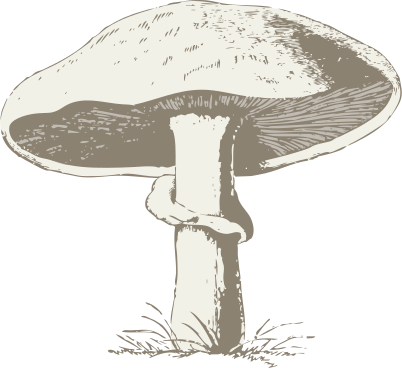
\includegraphics[width=.24\textwidth]{johnny_automatic_mushroom.pdf}
	\caption{Seta (\mushroom)}
	\label{fig:Seta}
\end{wrapfigure}
Al revisar la documentación sobre \mushroom\footnote{Ilustración obtenida en \url{https://openclipart.org/detail/900/two-mushrooms-by-johnny_automatic}} pudimos plantear mejor el problema que queríamos resolver, encontrar todas las \ARs presentes en un fichero "`pequeño"' que presenta estas características. En \href{https://archive.ics.uci.edu/ml/datasets/Mushroom}{UCI - Machine Learning Repository}\footnote{\url{https://archive.ics.uci.edu/ml/datasets/Mushroom}} describen su origen como



\selectlanguage{english}
\begin{quote}
   Mushroom records drawn from The Audubon Society Field Guide to North American Mushrooms (1981). G. H. Lincoff (Pres.), New York: Alfred A. Knopf 
\end{quote}
\selectlanguage{spanish}
\noindent Describen brevemente el contenido del fichero, indicando que se trata de setas clasificadas como comestibles o venenosas (primer valor de cada fila).
\selectlanguage{english}
\begin{quote}
\label{cita:incertidumbre-suprimida-en-mushroom}
   This data set includes descriptions of hypothetical samples corresponding to 23 species of gilled mushrooms in the Agaricus and Lepiota Family (pp. 500-525). Each species is identified as definitely edible, definitely poisonous, or of unknown edibility and not recommended. This latter class was combined with the poisonous one. The Guide clearly states that there is no simple rule for determining the edibility of a mushroom; no rule like ``leaflets three, let it be'' for Poisonous Oak and Ivy.
\end{quote}
\selectlanguage{spanish}
\noindent Y explican los valores que puede tomar cada uno de los atributos.
\selectlanguage{english}
\begin{quote}
   \footnotesize
   1. cap-shape: bell=b, conical=c, convex=x, flat=f, knobbed=k, sunken=s
   
   2. cap-surface: fibrous=f, grooves=g, scaly=y, smooth=s

   3. cap-color: brown=n, buff=b, cinnamon=c, gray=g, green=r, pink=p, purple=u, red=e, white=w, yellow=y

   4. bruises?: bruises=t, no=f

   5. odor: almond=a, anise=l, creosote=c, fishy=y, foul=f, musty=m, none=n, pungent=p, spicy=s

   6. gill-attachment: attached=a, descending=d, free=f, notched=n

   7. gill-spacing: close=c, crowded=w, distant=d

   8. gill-size: broad=b, narrow=n

   9. gill-color: black=k, brown=n, buff=b, chocolate=h, gray=g, green=r, orange=o, pink=p, purple=u, red=e, white=w, yellow=y

   10. stalk-shape: enlarging=e, tapering=t

   11. stalk-root: bulbous=b, club=c, cup=u, equal=e, rhizomorphs=z, rooted=r, missing=?

   12. stalk-surface-above-ring: fibrous=f, scaly=y, silky=k, smooth=s

   13. stalk-surface-below-ring: fibrous=f, scaly=y, silky=k, smooth=s

   14. stalk-color-above-ring: brown=n, buff=b, cinnamon=c, gray=g, orange=o, pink=p, red=e, white=w, yellow=y

   15. stalk-color-below-ring: brown=n, buff=b, cinnamon=c, gray=g, orange=o, pink=p, red=e, white=w, yellow=y

   16. veil-type: partial=p, universal=u

   17. veil-color: brown=n, orange=o, white=w, yellow=y

   18. ring-number: none=n, one=o, two=t

   19. ring-type: cobwebby=c, evanescent=e, flaring=f, large=l, none=n, pendant=p, sheathing=s, zone=z

   20. spore-print-color: black=k, brown=n, buff=b, chocolate=h, green=r, orange=o, purple=u, white=w, yellow=y

   21. population: abundant=a, clustered=c, numerous=n, scattered=s, several=v, solitary=y

   22. habitat: grasses=g, leaves=l, meadows=m, paths=p, urban=u, waste=w, woods=d
\end{quote}
\selectlanguage{spanish}

\noindent El fichero \mushroom\footnote{\url{https://archive.ics.uci.edu/ml/machine-learning-databases/mushroom/agaricus-lepiota.data}} es un fichero de texto con 8\,124 líneas, de las que muestro aquí las tres primeras:
\begin{quote}
   \footnotesize
   p,x,s,n,t,p,f,c,n,k,e,e,s,s,w,w,p,w,o,p,k,s,u
   
   e,x,s,y,t,a,f,c,b,k,e,c,s,s,w,w,p,w,o,p,n,n,g
   
   e,b,s,w,t,l,f,c,b,n,e,c,s,s,w,w,p,w,o,p,n,n,m
\end{quote}

\noindent El fichero \mushroom con el que llevo años trabajando está codificado de otro modo, conteniendo la misma información
\begin{quote}
   \footnotesize
   1 3 9 13 23 25 34 36 38 40 52 54 59 63 67 76 85 86 90 93 98 107 113
   
   2 3 9 14 23 26 34 36 39 40 52 55 59 63 67 76 85 86 90 93 99 108 114
   
   2 4 9 15 23 27 34 36 39 41 52 55 59 63 67 76 85 86 90 93 99 108 115
\end{quote}

Este modo de registrar información sobre los individuos de una población es muy habitual en todas las ciencias. Se determina qué \atributos se pueden medir, codificándolos mediante un número reducido de valores distintos, se observa a un \emph{individuo} y se mide el valor que toma en cada uno de los atributos seleccionados, obteniendo un vector de códigos.

\begin{Definition}[Individuo]
   Sean $A_i, i = 1 \ldots n$ un conjunto de atributos, siendo $n_i$ el número de valores distintos que puede tomar el atributo $A_i$. Definimos un \emph{individuo} como una $n$-túpla, un conjunto de $n$ valores obtenidos ordenadamente de los atributos $A_i$.
   $$individuo = \left(a_1, a_2\ldots a_n\right), a_i \in A_i$$
\label{def:individuo}
\end{Definition}

El propósito de recoger esta información suele ser el de \clasificacion, clasificar al \emph{individuo} en función de los valores observados en los atributos en estudio. Esta asignación se hace en función de la información que tenemos sobre esta población, generalmente un almacén \D como \mushroom, que contiene datos sobre muchos individuos de esta población correctamente clasificados.

Aunque es un problema de \Clasificacion se trata usando \arm por la forma en que se han codificado los valores expuestos para crear el fichero \mushroom. Se han utilizado números enteros consecutivos, los dos primeros para determinar la \clase (1 = \emph{venenosa}, 2 = \emph{comestible}), los siguientes para anotar el valor del atributo \texttt{cap-shape} (3 = \emph{convex}, 4 = \emph{bell}, 5 = \emph{sunken}, 6 = \emph{flat}, 7 = \emph{knobbed}, 8 = \emph{conical}), a continuación los valores del atributo \texttt{cap-surface} (9 = \emph{smooth}, 10, 11 y 12)\ldots Si encontramos \ARs fuertes entre los atributos y la \clase podemos intentar clasificar mejor a cualquier individuo de la población.







Esta estructura permite reducir notablemente la información a procesar para extraer reglas de asociación de estos ficheros, lo que convierte su estudio en una mera ejecución con \soporte mínimo nulo (si fueran más grandes podríamos averiguar antes si no están afectados por el \dilemaIR como se ha mencionado antes). Analicemos primero la estructura y veremos después una serie de características. Para entenderlo mejor analizaremos \mushroom, que es quien nos puso sobre la pista de que algo se hacía mal con este tipo de almacenes \D.

\begin{enumerate}
	\item Tiene 8\,124 filas (a las que hemos llamado \transacciones pero llamaremos \emph{registro} a partir de ahora).
	\item Cada registro tiene 23 elementos.
   \item El primer valor de cada registro es un 1 o un 2.
         
         El segundo valor es un 3, 4, 5, 6, 7 u 8.
         
         \ldots
         
         Esto nos hace pensar que cada posición del registro representa a una variable categórica. Y descubrir que los valores utilizados para representar a una variable no coinciden con los utilizados por el resto de variables, y que estos valores son consecutivos, 1\ldots119.
   % \item Si en una fila está el 1, entonces no está el 2. Esto mismo ocurre con los grupos \{3,4,5\}, \{6,7\},\ldots \{118,119\}. Esto nos hace pensar que son los valores de diferentes \atributos o \clases. Cada fila representa el valor que un individuo toma en un determinado atributo o \clase.
\end{enumerate}

%TODO: Esto va más adelante, fuera de la INTRO
En la primera lectura de \D, la que utilizamos para crear \aprioriC[1], podemos anotar la longitud de todas las \transacciones. De este modo será muy fácil comprobar si estamos trabajando con un \catalogo.

Esto sólo lo detectamos porque se han codificado los valores de cada variable categórica de modo que no haya dos iguales y sean todos consecutivos. Basta con aplicar el algoritmo mostrado en el listado~\ref{listado:comprobarCatalogo} para averiguar si \D contiene un \catalogo, una vez leído y obtenido \aprioriC[1] y $M$, el número de valores observado en todas las \transacciones.

\lstinputlisting[label=listado:comprobarCatalogo,
                 caption={Comprobación sobre \catalogos},
                 float=htb,
                 basicstyle=\footnotesize]
                 {./contenido/clasificacion/codigo/algComprobarCatalogo}


   % \item No hay dos registros iguales. Esto nos hace pensar que se trata de un \textbf{\catalogo}, no de una \textbf{muestra}. Aunque en ambos casos la reducción de información a procesar que podemos es la misma (en la muestra\ldots) la información que obtendremos no es la misma, lo que se explica en la sección~\ref{sec:3-3-CatalogoVsMuestra}.

Un \catalogo tiene una estructura muy rígida. Si hay valores missing se puede añadir un valor al atributo en cuestión indicando esa circunstancia, o no utilizar la información del atributo en cuestión o incluso hacer una estimación del valor si se puede justificar.

En un \catalogo todos los registros contienen $n$ datos, y si forma parte de una tarea de \clasificacion uno o varios de esos datos representan una \clase, generalmente el "`\atributo"' cuyo valor queremos determinar a partir de la observación de los valores del resto de \atributos.

\begin{Definition}[Registro]
   Sean $A_i, i = 1 \ldots n$ un conjunto de atributos, siendo $n_i$ el número de valores distintos que puede tomar el atributo $A_i$. Definimos un registro como una $n$-túpla, un conjunto de $n$ valores obtenidos ordenadamente de los atributos $A_i$.
   $$registro = \left(item_1, item_2\ldots item_n\right), item_i \in A_i$$
\label{def:registro}
\end{Definition}

\begin{Definition}[\Catalogo] Un \catalogo es un conjunto de $N$ registros diferentes.
   $$\catalogo = \left\{registro_i, i = 1\ldots N\ | \ registro_i \neq registro_j \forall i \neq j\right\}$$
\label{def:catalogo}
\end{Definition}
% \borrar{Buscar una definición mejor, en \clasificacion}


El número de combinaciones entre todos los valores de los atributos en estudio es muy grande, sin embargo cuando se está haciendo un estudio real no se obtendrán todas las combinaciones posibles. En un \catalogo sólo están las combinaciones que interesa estudiar, básicamente aquellas que sí se dan en la población en estudio. Es una selección de los registros que se podrían formar con todas las combinaciones de valores proporcionada por los atributos en estudio.

La esencia de un \catalogo es que no tiene registros repetidos. Si tomamos una muestra de una población midiendo en cada individuo todos los valores de los atributos del estudio es muy probable que en la muestra existan registros repetidos. Las muestras de este tipo se verán a fondo en la sección~\ref{sec:clasificacion:catalogo:muestras}, es importante estudiar sus diferencias con los \catalogos pues contienen información sensiblemente diferente.

Un \catalogo puede cambiarse fácilmente, basta con cambiar el número de valores que puede tomar una de las variables en estudio para que cambie por completo el \catalogo. Una muestra no puede cambiarse, se obtiene de la realidad, se diseña previamente y si se quiere añadir a otra muestra en que se han utilizado otros valores debería rehacerse\ldots


Si aprovechamos esta información podemos reducir notablemente los ítems a procesar sin perder la información que contiene el \catalogo (o muestra) completo\ldots

% \borrar{Aquí viene el ejemplo de Interacción'12, he de buscar cómo escribir código.}







%\subsection{\Catalogo comprimido}
%\label{sec:3-1-1-CatalogoComprimido}
%\input{./3-ARMCatalogos/3_1_Catalogos/3_1_1_CatalogoComprimido}
%
%
%
%
%
%
%
%\subsection{Lectura de \catalogo comprimido}
%\label{sec:3-1-2-LecturaDeCatalogoComprimido}
%\input{./3-ARMCatalogos/3_1_Catalogos/3_1_2_LecturaDeCatalogoComprimido}
%
%
%










Los catálogos son colecciones de registros preparadas para resolver informáticamente un problema de clasificación. Y muchos investigadores de esta especialidad publican sus datos para que otros investigadores puedan hacer pruebas con las mismas condiciones de partida: una colección de datos con ciertas características. En UCI, KEEL, LUCS\ldots encontraremos muchos catálogos entre los datasets que publican para resolver problemas de clasificación.\marginpar{\footnotesize Acabo de descubrir LUCS, que discretiza las colecciones de UCI y me ofrece 97 valores distintos en adult, frente a los 27\,245 que tiene el de UCI, he de analizarlo con mi código y EXPLICAR MEJOR LAS CONSECUENCIAS DE APLICAR ANTES O DESPUÉS MI MÉTODO O LA AGRUPACIÓN DE VALORES EN ATRIBUTOS NUMÉRICOS ya que se obtendrán reglas y catálogos completos bastante diferentes, esto da para otro artículo y más si tengo en cuenta que tiene datos missing por lo que puedo obtener catálogos completos usando menos atributos con más registros o catálogos completos usando sólo los atributos registrados en cada registro (a no ser que el análisis nos diga que cierto atributo no aporta información\ldots.}

Cuando no sabíamos que esos ficheros contenían catálogos intentábamos aplicar bien conocidos algoritmos de ARM pero no podíamos extraer información que contienen los datos porque se desbordaba la RAM del equipo en que se está aplicando el algoritmo y se abortaba el proceso tras horas de cálculos que finalmente no obteníamos. Esto nos sorprendía porque el primer catálogo que intentamos analizar con Apriori sólo tiene 5\,644 registros de 23 datos, no son números excesivos para un problema de Minería de Datos analizado con un ordenador de escritorio con cierta potencia y capacidad de RAM. Eso nos llevó a descubrir cómo se creó el catálogo a través de \url{UCI/mushroom}\ldots

Los catálogos caracterizan un problema de clasificación concreto. Si queremos plantear otro problema de clasificación, bien etiquetando a los mismos individuos en otras \clases o bien utilizando atributos diferentes no podemos utilizar directamente cualquier catálogo que tengamos sobre la misma población. Si los dos problemas usaran los mismos atributos pero diferentes \clases y las \clases en estudio son independientes no servirá de nada la información que tengamos sobre los catálogos completos del primer problema de clasificación si no sabemos analizar qué información puede ser relevante y cuál no, de hecho la información menos relevante en esta situación es la distribución de las \clases en cada uno de los problemas de clasificación por lo que debemos huir de interpretaciones erróneas utilizando estos datos para estimar soportes o confianzas poblacionales.

De un catálogo se puede extraer información válida para otro problema de clasificación que utilice los mismos atributos ya que si en la muestra en que se basa el catálogo no presenta cierta relación entre los valores de los atributos YA SABEMOS QUE NO APARECERÁ ESA RELACIÓN AUNQUE CAMBIEMOS DE CLASES (siempre que el catálogo sea válido, aún tengo que hacer muchas definiciones sobre muestra, población, distribución de \clases, problema de \clasificacion, \atributos, \clases, \catalogos, catálogos completos, validez de un catálogo\ldots).

Aunque la \ARM busca cualquier relación entre cualquier par (o $k$-itemset) de valores de \D, el objetivo del problema de \clasificacion es siempre el mismo, etiquetar cada \registro con una \clase basándose en la información disponible sobre otros \registros con valores idénticos en sus \atributos.





\subsection{Muestras}
\label{sec:clasificacion:catalogo:muestras}
La importancia que se da en todos los estudios de \ARM al \soporte de una \ar se justifica cuando se trabaja con muestras, que no contienen la misma información que un \catalogo. Para obtener una muestra en un problema de \clasificacion se han de seleccionar individuos de una población, medir en cada uno de ellos el valor que toma cada uno de los \atributos en estudio y averiguar la \clase a la que pertenece. Al guardar todos los \registros obtenidos de este modo es posible que existan \registros repetidos, lo que aporta información sobre la distribución de la población en estudio con un elevado coste sobre los \catalogos ya que en estos no deberíamos repetir el registro si no añadir un número entero indicando el número de veces que aparece el \registro en la muestra.






\section{\CC}
\label{sec:clasificacion:catalogo-completo}
% !TEX root = ../../Lazcorreta.Tesis.tex
\ABIERTO
Al seguir trabajando con \mushroom encontramos otra versión del mismo dataset en KEEL

http://sci2s.ugr.es/keel/dataset.php?cod=178


\borrar{Necesito definir antes conjuntoDeValoresDeAtributos, quizá en otra sección.}
\begin{Definition}[\CC] Un \CC es un \catalogo sin incertidumbre.
   $$\CC = \left\{registro_i, i = 1\ldots N\ | \ registro_i \neq registro_j \forall i \neq j\right\},  conjuntoValoresAtributos son todos diferentes$$
\label{def:catalogo}
\end{Definition}






\subsection{Colecciones de \CCs}
\label{sec:clasificacion:catalogo-comprimido:colecciones}
%\input{contenido/clasificacion/catalogo-comprimido/colecciones}

Todos los \CCs pueden tener un \CC maximal y diversos \CCs de menores dimensiones. Volviendo al origen de esta investigación, disponemos de un dataset\ldots





%TODO: Añadir \missing al índice alfabético
\section{Datos missing}
\label{sec:clasificacion:datos-missing}
% !TEX root = ../../Lazcorreta.Tesis.tex
\ABIERTO
%TODO: Incluir "datos missing" en indice-alfabetico
\mushroom contiene 8\,124 registros en su dataset original de la UCI, sin embargo en el fichero KEEL con el que hemos trabajado desde la sección~\ref{sec:catalogo:catalog} contiene sólo 5\,644 registros porque se han eliminado los \registros con datos missing que contenía el fichero original. Para diferenciar ambos \datasets llamaremos \texttt{mushroom-original} al \dataset de la UCI y \texttt{mushroom-reducido} al que no contiene datos missing.

En un problema de \dm los datos missing no deberían ser considerados. El objetivo de esta disciplina es la obtención de información (previamente desconocida) a partir de los datos. Un dato missing no aporta información como dato, podría ser interpretado en muchos experimentos el hecho de no conocer ese dato pero el dato en sí no lo conocemos y, por lo tanto, no podemos usarlo. Se podrían estimar a partir de los datos que sí conocemos pero si no hay una justificación suficientemente poderosa no deberíamos "`inventar"' ningún valor cuando queremos obtener la información que contienen los datos que realmente conocemos. La \dm se aplica a los datos conocidos o estimados pero en este momento sólo tenemos datos missing sin interpretar por lo que no nos pueden dar ningún tipo de información.

Cualquier \ar que incluya el ítem \texttt{stalk-root=?} en su antecedente debe ser ignorada ya que su interpretación sería "`\emph{Si no sé qué valor tiene stalk-root entonces\ldots}"'.

%TODO: He cambiado la referencia a catalogo-comprimido por catalogo-completo. Comprobar que es correcto.
En un registro, la ausencia de un dato provocará tener un valor menos, lo que traducido a transacciones se convierte en una transacción de distinto tamaño que el resto de registros. Esto sería un problema para tratarlo como se ha propuesto en la sección~\ref{sec:clasificacion:catalogo-completo} ya que el fichero \D no será considerado \catalogo por no tener todos sus registros el mismo tamaño. Una solución consiste en considerar el valor missing de un atributo como un valor distinto al resto de los que realmente contiene, en el caso de \mushroom se denota con \texttt{?}, al convertirlo en fichero \D se codificará ese valor como un valor distinto del atributo al que pertenezca y la única consecuencia es, aparentemente, que tenemos un ítem diferente más.

Los datos missing son difíciles de interpretar correctamente ya que para convertir los ficheros en formato adecuado para ARM se utiliza un código binario para indicar esta situación, i.e., si un registro no contiene información sobre un atributo se crea la categoría ficticia "`dato desconocido"' en dicho atributo y se le asigna esa categoría, así podemos aplicar con cierta normalidad las técnicas de ARM, aunque la interpretación de las reglas que se pueden obtener es confusa:

\begin{quote}
Si no conocemos el valor del atributo $\A_i$ podemos deducir que\ldots
\end{quote}

Eliminar los registros con datos missing parece una estrategia correcta para no tener que gestionar estas \ars. Sin embargo perdemos información sobre 2\,480 registros, sin saber si la información que perdemos es relevante o no lo es.

Si analizamos el fichero \mushroom observaremos que sólo un atributo contiene datos missing, \texttt{stalk-root}, y ya hemos visto en la sección~\ref{sec:clasificacion:catalogo-completo} que este atributo es prescindible, al menos en el dataset reducido de KEEL. Con lo que ahora sabemos sobre \catalogos podemos diseñar otra estrategia, eliminar el atributo \texttt{stalk-root} del dataset original y comprobar si esos 2\,480 registros ignorados por la estrategia utilizada contienen información que habíamos perdido irremediablemente.

En \urlConNotaAlPie{http://sci2s.ugr.es/keel/dataset.php?cod=178}{KEEL - Mushroom} proporcionan dos ficheros \mushroom:
\begin{itemize}
  \item por defecto el que han elaborado con su formato tras eliminar los registros con datos missing, con 5\,644 registros\footnote{\scriptsize\url{http://sci2s.ugr.es/keel/dataset/data/classification/mushroom.zip}},
  \item si lo buscamos nos ofrecen el dataset original en formato KEEL, con 8\,124 registros\footnote{\scriptsize\url{http://sci2s.ugr.es/keel/dataset/data/missing/mushroom.zip}}.
\end{itemize}
Al analizar ambos ficheros se obtienen los siguientes resultados:
\begin{enumerate}
  \item \texttt{mushroom-original} contiene un \sCC de 8\,124 \registros, con un atributo que contiene datos missing, \texttt{stalk-root}, que es prescindible y no aumenta el tamaño del \catalogo.
  \item \texttt{mushroom-reducido} contiene un \sCC de 5\,644 \registros, \texttt{stalk-root} es prescindible y no aumenta el tamaño del \catalogo.
\end{enumerate}
Luego tenemos dos análisis sobre dos \datasets que ofrecen datos similares pero deben contener diferente información. Analizar sus similitudes y diferencias nos dará más información que la que obteníamos con el primer fichero KEEL. Destaquemos que:

\begin{enumerate}
  \item Ambos ficheros son \sCCs. Todos sus \registros son distintos y no contienen incertidumbre.
  \item Si eliminamos en cualquiera de ellos el atributo \texttt{stalk-root} no se reduce el \catalogo ni se pierde información. No sabemos si \texttt{mushroom-reducido} seguirá siendo un \sCC.
\end{enumerate}
Si no sobran los 2\,480 registros de más que tiene el \CC original deberían de aportar algo de información que no está presente en el \catalogo reducido. Esto lo sabremos tras eliminar su atributo \texttt{stalk-root} y comprobar si genera incertidumbre\borrar{Explicarlo con ecuaciones}.
\begin{itemize}
  \item Si no la genera es por\ldots
  \item Si la genera es por\ldots
\end{itemize}



Si eliminamos \texttt{stalk-root} de ambos ficheros obtendremos dos \sCCs distintos, el primero con todos los registros-tipo del segundo y además 2\,480 registros-tipo que no están en el segundo. Es evidente que el primero tiene información más precisa sobre el problema de \clasificacion que estamos analizando. Pero la información extra que contiene no es sobre el atributo \texttt{stalk-root}, ni tan siquiera se utiliza este atributo para obtener esa información, sólo depende de las co-ocurrencias entre valores del resto de atributos. Si eliminamos el atributo \texttt{stalk-root} de ambos ficheros obtendremos dos nuevos \sCCs, esta vez sin datos missing, ambos orientados al mismo problema de \clasificacion y sin ninguna discrepancia entre ellos (de hecho el reducido es una partición del original). Si pudiéramos utilizar cualquiera de ellos en nuestro próximo clasificador está claro que deberíamos usar el \sCC que ese obtiene eliminando el atributo \texttt{stalk-root} al dataset original.

El \sCC mayor contiene al menor pero el menor se ha obtenido a partir de la información proporcionada por otro atributo (que ahora ya no está). Ambos contienen algo de información distinta para el mismo problema de \clasificacion. En el menor hay más $ARN_2$, que desaparecen al añadir nuevos registros-tipo para formar el mayor, es lo que podría ocurrir si seguimos tomando muestras y aparecen nuevos registros-tipo que no presenten incertidumbre, el \sCC va mejorando y nos informa que los datos que conocemos garantizan una buena clasificación (no es necesario medir otro atributo porque no tenemos incertidumbre y cada vez sabemos más sobre los registros-tipo de este problema de clasificación).







No todos los \catalogos con datos missing tendrán las mismas características que \mushroom, pero sí se puede dar en muchos estudios que sigamos añadiendo registros a un dataset pero sin incluir el valor de uno de sus atributos, si el resto de atributos es suficiente para clasificar correctamente al individuo tendremos una situación similar a la analizada en esta sección. Si estamos trabajando con un \sCC completo y válido es muy posible que no necesitemos nunca más medir el valor de ese atributo, pero no deberíamos borrarlo del dataset original porque alguna vez podría aparecer algo de incertidumbre en el \catalogo y sería útil poder añadir toda la información que ya se recogió en su día sobre cualquier otro atributo medible en los individuos en estudio.






\section{Publicaciones}
\label{sec:clasificacion:publicaciones}
% !TEX root = ../../Lazcorreta.Tesis.tex
En Interacción'12 comenzamos a publicar nuestros resultados sobre las colecciones de \transacciones estructuradas mediante \catalogos. Los mayores avances los hemos obtenido este último año y estamos en un proceso actual de publicación de resultados en diversas revistas y un nuevo congreso internacional.





%\cite{Lazcorreta:Botella:FCaballero:EfficientAnalysisOfTransactionsWebRecommendations:2012}
\subsection*{Efficient analysis of transactions to improve web recommendations, 2012}

\begin{quote}
  Lazcorreta Puigmartí, E., Botella Beviá, F. y Fernández-Caballero, A. Efficient analysis of transactions to improve web recommendations. {\em Actas del XIII Congreso Internacional de Interacción Persona-Ordenador}, ACM International Conference Proceeding Series, 2012. \leePDF{bib/nuestros/LazcorretaBotellaFCaballero-EfficientAnalysisOfTransactionsWebRecommendations-2012.pdf}
\leePDF{bib/nuestros/LazcorretaBotellaFCaballero-AnalisisEficienteDeTransacciones-2012-Presentacion.pdf}
\scopus{http://www.scopus.com/inward/record.url?eid=2-s2.0-84869053054&partnerID=40&md5=ded243c196907c1e6eec90cd9624ab3d}
\descargaRevisado{https://www.researchgate.net/publication/266652926_Efficient_analysis_of_transactions_to_improve_Web_Recommendations}
\descargaRevisado{https://www.deepdyve.com/lp/association-for-computing-machinery/efficient-analysis-of-transactions-to-improve-web-recommendations-mBuBBNIv7c}
\github{https://github.com/EnriqueLazcorreta/tesis-0/blob/master/bib/nuestros/LazcorretaBotellaFCaballero_EfficientAnalysisOfTransactionsWebRecommendations_2012.pdf}
\github{https://github.com/EnriqueLazcorreta/tesis-0/blob/master/bib/nuestros/LazcorretaBotellaFCaballero_AnalisisEficienteDeTransacciones_12_Presentacion.pdf}
\end{quote}

\begin{quotation}
	\noindent\textbf{Resumen}

	\nopagebreak When we deal with big repositories to extract relevant information in a short period of time, pattern extraction using data mining can be employed. One of the most used patterns employed are Association Rules, which can measure item co-occurrence inside large set of transactions. We have discovered a certain type of transactions that can be employed more efficiently that have been used until today. In this work we have applied a new methodology to this type of transactions, and thus we have obtained execution times much faster and more information than that obtained with classical algorithms of Association Rule Mining. In this way we are trying to improve the response time of a recommendation web system in order to offer better responses to our users in less time. Copyright 2012 ACM.
\end{quotation}








\subsection{[...]}
En la actualidad estamos completando la redacción de un artículo sobre esta fase de nuestra investigación, que será enviada en breve para su revisión y posible publicación en revista. En él se exponen la teoría y experimentos que forman la sección~\ref{sec:clasificacion:catalogo-completo}.




\subsection{[...]}
La Interacción Persona-Ordenador es una disciplina en la que se analizan muchos catálogos por lo que presentaremos nuestra aportación a esta rama de la ciencia en el Congreso Internacional Interacción'16, que se celebrará en septiembre de 2016 en Salamanca.





\chapter{Conclusiones y Trabajo Futuro}
\label{chap:conclusiones-y-trabajo-futuro}
% !TEX root = ../Lazcorreta.Tesis.tex
\noindent Las mejores ideas expuestas en esta tesis son muy simples. Desde el primer algoritmo que entra en juego, Apriori, hasta la elaboración de catálogos completos ínfimos son ideas muy simples que implementadas de forma eficiente pueden hacer lo que se le pide a la Minería de Datos: buscar una aguja en un pajar.

Los catálogos completos tienen un potencial fácil de descubrir mediante sencillas técnicas informáticas de Minería de Datos. Este trabajo presenta una teoría en torno a un tipo de datos muy utilizado que posibilita la obtención extrema de la información que contienen grandes colecciones de datos utilizando la tecnología actual en tiempo real. 

Los datos bien recogidos reflejan el estado actual del mundo que nos rodea, por eso es importante poder analizarlos rápidamente utilizando en algunos casos información histórica sobre el mismo problema o bien partiendo de un nuevo problema y analizando rápidamente las características de los datos que proporciona su estudio. Si sabemos qué puede descubrir la Minería de Datos a partir de la observación de los datos que hemos recogido podremos crear algoritmos que descubran lo que estamos buscando en tiempo real y con un uso aceptable de recursos de un servidor dedicado.

Este trabajo presenta unos antecedentes que encaminan al investigador a descubrir, quizá por casualidad, las características especiales de un modelo matemático de almacenamiento de información y el uso que se está dando a estas colecciones de datos por parte de especialistas en el problema de clasificación. La aparición del problema del Minado de Reglas de Clasificación Asociativas en [\ldots] era previsible, todas las reglas de asociación tienen un aspecto muy simple que sugiere a cualquier investigador que puede ser utilizado en el problema de clasificación. El hecho de que yo, especializado en el problema de asociación, observara los mismos datos que los especialistas en clasificación tendría que llevarnos al mismo resultado si ellos habían alcanzado el óptimo o a un mejor resultado si yo era capaz de aportar ideas sobre cómo utilizar los elementos de ARM.

El primer descubrimiento simple y útil de esta tesis son los \emph{catálogos comprimidos} expuestos en la sección~\ref{sec:catalogos:catalogo-comprimido}. Con ellos descubrí que el modo de aplicar técnicas de ARM en los artículos que consultaba no era del todo correcto  [\ldots]. No soy especialista todavía en el Problema de Clasificación por lo que algunas conclusiones de esos artículos y, sobre todo, las pruebas de eficiencia de los algoritmos que proponían, estaban fuera de mi alcance. Se me ocurrió incorporar las restricciones iniciales del problema de clasificación a un problema general de asociación. Los problemas de asociación se resuelven mediante la fuerza bruta leyendo todos los datos que tenemos y mirándolos desde distintas perspectivas, si quiero resolver un problema distinto, un problema de clasificación, usando técnicas de minería de reglas de asociación debería aprovechar, al menos, la rígida estructura de los datasets usados para clasificación (en asociación sólo hay una norma: en un registro no se cuentan los datos repetidos, lo que hace que el número de reglas de asociación que se puede buscar sea tan grande que provoque desbordamiento de memoria en los programas que intentan analizar grandes colecciones de datos). Se me ocurrió que si todos los registros han de tener un valor para cada uno de los atributos en estudio podía reducir el número de datos a procesar y las dimensiones del dataset eliminando únicamente un valor de cada atributo en todo el dataset. Al hacerlo y comprobar que la nueva colección de datos, compresión sin pérdidas de la colección original, sí se podía analizar utilizando el clásico Apriori y obtener todas las reglas de asociación que contenía empecé a asimilar mejor las características de un catálogo.

Primero descubrí características matemáticas, restricciones teóricas que me permitían reducir las dimensiones del problema original y, usando muchos recursos, obtener toda la información que contienen esas pequeñas colecciones de datos en cuanto a reglas de asociación se refiere. Pero tenía que haber algo más, las características matemáticas que utilicé en~\ref{sec:catalogos:publicaciones} me exigían usar muchos recursos y no me ofrecían información demasiado relevante, además seguía necesitando mucha RAM para trabajar con colecciones pequeñas de datos, a pesar de que ya sabía que contenían muchísima información. Quería encontrar mejor información en menos tiempo y usando menos RAM por lo que introduje la STL a mi desarrollo y comprobé en la primera aplicación que la teoría de conjuntos tenía mucho que aportar al análisis de catálogos.

% !TEX root = ../Lazcorreta.Tesis.tex

Tantos años de trabajo han dado lugar a muchas ideas teóricas sobre la aplicación de técnicas de DM por lo que quedan abiertas muchas líneas de investigación que podrían ser continuación de este trabajo. Como \emph{trabajar a nivel de \texttt{bits}} buscando la máxima eficiencia en el uso informático de grandes colecciones de datos, o \emph{profundizar en el desarrollo de Clasificadores}, de \emph{lógica difusa para agrupación de valores en atributos numéricos o de amplios rangos} y de tantas otras cosas que han ido apareciendo en el estado del arte de esta tesis y que no he podido abarcar para centrarme en obtener algo tangible mediante el método científico.

La investigación mostrada en el último capítulo de esta tesis está avalada por su implementación en el campo de la Minería de Datos utilizando la tecnología actual.
\marginpar{\footnotesize Es evidente que tengo que reescribir este párrafo. La idea es interesante pero\ldots}
El preproceso de cualquier catálogo permite crear colecciones de catálogos que pueden ser utilizadas en tiempo real en grandes problemas de clasificación que pueden ser escalados sin tener que renunciar en cada nuevo estudio a todo el conocimiento adquirido en estudios sobre las mismas clases. En este trabajo se ha demostrado que cualquier subconjunto de un catálogo completo puede ser tratado como catálogo completo considerando siempre la incertidumbre que puede contener, si quisiéramos utilizar los datos de un problema de clasificación en otro problema de clasificación con otras clases podríamos comenzar con los registros-tipo del primer catálogo, todos los que puedan ser clasificados en el segundo problema se incorporan al catálogo del segundo problema pero así no  voy bien, lo que quería decir es que si empezamos con el menor de todos los catálogos ínfimos y vamos catalogando en la segunda clase todos sus registros podemos llegar a no tener incertidumbre (caso ideal y poco probable si la segunda clase es independiente de la primera, dato interesante) pero al menos si tenemos incertidumbre es posible que sea poca, si hacemos lo mismo con otros catálogos ínfimos podríamos descubrir qué atributos aportan más determinación al segundo problema y plantear un catálogo inicial para el segundo problema.



\appendix

\chapter{Notación}
\label{apdx:notacion}
% !TEX root = ../Lazcorreta.Tesis.tex
La notación usada en este informe se ha intentado ajustar a la más utilizada en la bibliografía revisada a lo largo de estos años de investigación. Por este motivo no es uniforme en los tres capítulos de investigación en que se divide esta tesis.

\section{Sistemas de Recomendación Web}
En este capítulo\ldots




\section{Minería de Reglas de Asociación}
En este capítulo\ldots




\section{Catálogos}
En este capítulo\ldots






\chapter{Código}
\label{apdx:codigo}
% !TEX root = ../Lazcorreta.Tesis.tex
Se ha desarrollado mucho código para poder comprobar todo lo que se afirma en esta tesis. Se ha trabajado del modo más estándar posible para conseguir un código eficiente y que pueda ser incorporado a otras investigaciones. Se publicará como código abierto bajo la licencia\ldots en\ldots




\section{Sistemas de Recomendación Web}
En este capítulo\ldots




\section{Minería de Reglas de Asociación}
En este capítulo\ldots




\section{Catálogos}
En este capítulo\ldots






\chapter{Datos utilizados}
\label{apdx:datos-utilizados}
% !TEX root = ../Lazcorreta.Tesis.tex
Para llevar a cabo las pruebas de rendimiento y aplicabilidad de nuestras propuestas se han usado datos propios y datos procedentes de diferentes \datasets públicos como UCI, KEEL, LUCS-KDD\ldots





\section{Sistemas de Recomendación Web}
En este capítulo usamos datos de un servidor propio con la intención de poder utilizar las recomendaciones sugeridas por nuestra metodología en el servidor del que se obtuvieron. Son los ficheros \texttt{TAL} y \texttt{CUAL} que no publicaremos por carecer de interés su contenido, ya que el servidor del que se obtuvieron ya no está disponible y no se podría dar ninguna interpretación a los resultados obtenidos\ldots

También usamos \texttt{TAL}\ldots




\section{Minería de Reglas de Asociación}
En este capítulo seguimos trabajando con los mismos datos que en el anterior e incorporamos\ldots




\section{Catálogos}
En este capítulo es en el que más opciones hemos tenido a la hora de seleccionar datos y probar la eficiencia y posibilidades de nuestros desarrollos. Existen muchos \datasets públicos bien documentados sobre el diseño y contenido de estos \datasets y es una información que enriquece mucho la investigación\ldots






\chapter{Sobre la bibliografía}
\thispagestyle{empty}
\label{chap:sobre-la-bibliografia}
% !TEX root = ../Lazcorreta.Tesis.tex
\ABIERTO

%La bibliografía de este informe es una selección de todos los artículos que he consultado durante mi investigación. Es muy probable que haya olvidado citar algún artículo que aporte valor a la presente investigación por lo que he añadido en el DVD complementario a este informe una copia de la \db bibliográfica que he gestionado durante estos años. Se trata del fichero \texttt{bib/tesis.bib}.

Todas las citas bibliográficas que figuran en este informe, tanto de trabajos propios como de otros investigadores, contienen enlaces externos que han sido revisados entre noviembre y diciembre de 2015. Para no perder las direcciones utilizadas en la versión impresa se han añadido en forma de notas a pie de página, aunque algunas URLs sean difíciles de reproducir a mano.

Se han utilizado diferente imágenes\footnote{Obtenidas de \href{http://sourceforge.net/projects/openiconlibrary/}{http://sourceforge.net/projects/openiconlibrary/}, una completa librería de iconos e imágenes de código abierto.} para indicar los recursos adicionales sobre la bibliografía utilizada que he ido recopilando a través del proceso de investigación. En la versión impresa aparecen a modo informativo, describiendo visualmente la información adicional que contiene cada elemento bibliográfico.
 
\begin{itemize}
	\item[\iconoPDF] indica que hay una copia del artículo, resumen o presentación en el \dvdAdjunto que complementa esta tesis, en formato \texttt{.pdf}, en alguna de las carpetas de \texttt{bib}. Sólo es útil si se está revisando este documento desde el \dvdAdjunto adjunto o desde una copia de este documento colocada junto a una copia de la carpeta \texttt{bib} del \dvdAdjunto.
  %\item[\iconoDescargaPDF] enlaza a la URL en que se encuentra publicada la referencia, en formato \texttt{.pdf}.
  \item[\iconoDescarga] enlaza a la URL desde la que se puede descargar el artículo.
  \item[\iconoWWW] enlaza a la URL con información sobre la referencia.
  \item[\iconoSCOPUS] enlaza a la URL de \url{http://www.scopus.com} con información sobre la referencia. Requiere acceso identificado, en mi caso proporcionado por mi universidad.
  \item[\logoCIO] enlaza a la URL con el documento publicado como \textsl{Working Paper} para el Instituto Universitario Centro de Investigación Operativa de la Universidad Miguel Hernández de Elche.
  \item[\logoGitHub] enlaza a la URL en que he publicado este informe o la parte de él que se cita.
\end{itemize}

También están en el \dvdAdjunto adjunto las tres bases bibliográficas que he utilizado en este informe, todas ellas en la carpeta \texttt{bib} y con formato \BibTeX. En ellas encontrará el lector más información que la expuesta en este informe. He utilizado los gestores bibliográficos \texttt{JabRef}  \footnote{\includegraphics[height=10pt]{./imagen/JabRef} \url{http://jabref.sourceforge.net/}} y \texttt{BibDesk} \footnote{\includegraphics[height=10pt]{./imagen/bibDeskIcon} \url{http://bibdesk.sourceforge.net/}} pero por tratarse de ficheros de texto plano pueden abrirse con múltiples aplicaciones. Se incluye también la base bibliográfica \texttt{tesis.bib}, en la que se encuentran la mayoría de artículos que he utilizado a lo largo de estos años para documentarme sobre el estado del arte de la materia tratada. No se han incluido en este informe todas estas referencias pero no quería que todos estos autores y artículos se olvidaran pues de ellos extraje mucho conocimiento en su día.

Todos los artículos incluidos en formato \texttt{.pdf} han sido descargados sin usar servicios de pago por lo que asumo que su utilización a través de la edición digital de este informe no infringe ninguna licencia de uso. Personalmente me ha resultado muy productivo tener preparados estos enlaces para elaborar un informe de mayor calidad y espero que al lector le sea útil para tener a mano mucha más información sobre los temas tratados en esta tesis.



\setcounter{footnote}{0}
% \bibliography{bib/TesisEnriqueLazcorreta,bib/CitanApriori2}
%\defaultbibliographystyle{alpha} %alphadin
% \bibliographystyle{plainnat} %plainnat alpha unsrtnat abbrvnat apalike-es
% \thispagestyle{empty}
\printbibliography
\addcontentsline{toc}{chapter}{Bibliografía}


% {
\cleardoublepage
% \small
% \stepcounter{chapter}
\phantomsection
\printindex
% }


\end{document}